\documentclass[a4paper,10pt,twocolumn]{article}
\usepackage{helvet}
\renewcommand*\familydefault{\sfdefault}
%% Language and font encodings
\usepackage[english]{babel}
\usepackage[utf8x]{inputenc}
\usepackage[T1]{fontenc}

%% Sets page size and margins
%\usepackage[a4paper,top=3cm,bottom=2cm,left=3cm,right=3cm,marginparwidth=1.75cm]{geometry}
\usepackage[a4paper,top=2cm,bottom=2cm,left=1.5cm,right=1.5cm,marginparwidth=1.75cm]{geometry}

%% Useful packages
\usepackage[round]{natbib}
\usepackage[dvipsnames]{xcolor}
\usepackage{sectsty}
\usepackage{amsmath}
\usepackage{graphicx}
\usepackage[colorinlistoftodos]{todonotes}
\usepackage[colorlinks=true, allcolors=blue]{hyperref}
%\usepackage{subfigure}
\usepackage{soul} % strikethrough
\usepackage{floatrow}
\usepackage{hyperref}

\sectionfont{\color{Mahogany}}
\subsectionfont{\color{Mahogany}}

% Left justified title
\usepackage{etoolbox}
\makeatletter
\patchcmd{\@maketitle}{\begin{center}}{\begin{flushleft}}{}{}
\patchcmd{\@maketitle}{\begin{tabular}[t]{c}}{\begin{tabular}[t]{@{}l}}{}{}
\patchcmd{\@maketitle}{\end{center}}{\end{flushleft}}{}{}
\makeatother

% Supplement
\newcommand{\beginsupplement}{%
        \setcounter{table}{0}
        \renewcommand{\thetable}{S\arabic{table}}%
        \setcounter{figure}{0}
        \renewcommand{\thefigure}{S\arabic{figure}}%
     }

%\title{\textbf{Why deconvolve Ca\textsuperscript{2+}? \\ \large A practical guide to recovering neural activity from cellular fluorescence imaging}}
\title{\textbf{On the use of calcium deconvolution algorithms in practical contexts}}

\author{Mathew H. Evans, Rasmus S. Petersen \& Mark D. Humphries}

\begin{document}
\maketitle

\begin{abstract}
% 11/09/18 N.B. We need to talk about de-noising vs deconvolution (into ~FR) vs spike inference. Sparse deconvolution (e.g. Pachitariu) approximates spike inference at the imaging frame rate.

\textbf{{\color{MidnightBlue}
Fluorescence imaging of somatic calcium (Ca\textsuperscript{2+}) is an increasingly popular technique for recording the activity of large groups of neurons. Recent efforts have seen an explosion in the number of available methods for Ca\textsuperscript{2+} deconvolution and spike inference to improve signal quality, with impressive results.
%Fluorescence imaging of somatic calcium (Ca\textsuperscript{2+}) is an increasingly popular technique for recording the activity of large groups of neurons. To improve signal quality the fluorescence time-series is typically de-noised and deconvolved prior to analysis. Deconvolved Ca\textsuperscript{2+} is an indirect measure of spiking activity, therefore some methods go further and infer the timing and number of spikes underlying the Ca\textsuperscript{2+} trace. Recent efforts have seen an explosion in the number of available methods for Ca\textsuperscript{2+} deconvolution and spike inference, with impressive results.
Here we evaluate this progress by comparing the performance of deconvolution algorithms in practical contexts.
We find that good estimates of spike rate can be recovered on ground truth data, but only if spike-inference methods are tuned to individual cell properties. We show that a commonly used metric - Pearson Correlation Coefficient - yields widely ranging results with small changes in parameters, and poor estimates of firing rate when compared to a spike-based metric. When analysing large-scale recordings from behaving mice, state-of-the-art methods are inconsistent and perform poorly when using parameters tuned to ground truth data. Estimates of event rate, silent cells, tuned cells, dimensionality and correlation distributions vary widely between methods and are affected by parameter choices. We conclude that to date there are no `magic bullet' approaches for inferring accurate estimates of neural activity from fluorescence imaging data. We suggest that conclusions of analyses that depend on deconvolution or spike-inference must be verified across multiple methods and analysis parameters. [Currently $\sim$220 words. Needs to be closer to 150.]}}
\end{abstract}
% We conclude that the purported advantages of deconvolution may not outweigh the disadvantages of losing information and introducing noise. }}
%\emph{I.E. disagreement between methods (re FR, 'tuned', correlations, dimensionality), poor recovery of temporal tuning}. 
%Some notes on our efforts to compare calcium deconvolution methods. After describing a different spike distance metric (Victor \& Purpura 1996), we outline the different deconvolution methods attempted and compare their results on ground truth and example `real' data.


\section{Introduction}
Imaging is cool and increasingly popular. 

%\textbf{why deconvolve} \\
%- improve signal/noise ratio i.e. better estimate what the cell is doing\\
%- increase temporal resolution e.g. to recover tuning and correlations\\
%- normalisation of expression across neurons\\
%- get rid of known artefacts\\

However the signal has a number of known artefacts. Background noise and neuropil subtraction. Slow calcium kinetics. Difference in expression across cells. Known experimental artefacts (movement). Deconvolution is a process designed to elevate these problems. 

Deconvolved Ca\textsuperscript{2+} is an indirect measure of spiking activity, therefore some methods go further and infer the timing and number of spikes underlying the Ca\textsuperscript{2+} trace.

%\noindent \textbf{how to deconvolve}\\
%- many methods giving different results (due to analysis/design choices)\\
%- comparing methods involves metrics\\
%- metrics are important as they give different results.\\
%- PCC is commonly used due to its perceived interpretability \citep{Theis2016-ee}, and common use as a metric of model fit across neuroscience.\\
%- Spikefinder showed many state of the art methods perform equally well if assessed by PCC. 

Recent community efforts have shown great progress in the speed, scale, and accuracy of deconvolution and spike-inference methods under idealised conditions \citep{Berens2018-su}, but how well do they work in real-world experiments?

An important aspect of comparing performance of different methods is the chosen metric. Pearson Correlation Coefficient (PCC) is commonly used due to its perceived interpretability \citep{Theis2016-ee}, and common use as a metric of model fit across neuroscience. While different methods give varying results due to analysis and algorithm design choices, they may appear to converge when assessed with PCC \citep{Berens2018-su}. 

OR how much of this convergence is due to using PCC as a metric?




%\noindent \textbf{the cautionary tale}\\
%- if the signal isn't perfect our metrics and methods lead to biased/poor estimates of simple neural properties (FR, tuning, correlations)\\
%- this bias may be worse (more wrong) than the benefits we're supposed to get when deconvolving e.g. miss-classify cells as tuned/silent. Poor estimates of data dimensionality. \\
%- artefacts may not be removed after all\\

Here we set to assess the performance of state of the art spike inference and deconvolution methods in real-world contexts. On ground truth data, we show that the metric used for fitting parameters affect the ability to recover simple measures of neural activity such as firing rate. On large-scale imaging data we show that ground-truth derived parameters lead to biased estimates of firing rates. Further, different methods disagree on simple measures such as the number of silent or tuned cells, and dimensionality. In addition, artefacts in the data are not automatically removed. 






%\emph{The point of this section is that if you are going to do deconvolution, PCC is a biased metric so use something else e.g. ER. This isn't a particularly novel point any more - see Reynolds biorxiv 2017 + Ganmor}\\

%\emph{MDH: as hinted in the Abstract, if our narrative here is the comparison of algorithms, then this section will be written as a comparison on ground truth, not as a “failure”.}

%\emph{So we show that the common cost function (Pearson) fails to properly fit the algorithms no matter which algorithm we use. But if we use a different cost function (ER), each deconvolution and inference algorithm can fit the ground truth well. So no difference between algorithms if we choose the right cost function.  so in principle, these algorithms can work. But, they have to be tuned for each neuron; so, what happens when we try to use them for real data with no ground truth?}

%\noindent \emph{\textbf{Results in brief}\\
%- Using PCC as a metric leads to poor estimation of firing rate, both under and over estimation, out by a factor of 1 (double the true firing rate)\\
%- PCC does not vary smoothly with model parameters, potentially leading to poor (over) fitting to training data N.B. we didn't test this - all data was used for fit + evaluation, not separate training/test sets.\\
%- ER is a better choice (but see also CosMIC, Reynolds et al 2017 or Information based methods, Theis)\\
%- This result is true regardless of method used (see repeated analysis on MLSpike and LZero\\
%- This result is true on both high and low frame rate data}




%\begin{figure}%[h!]
%\centering
%\subfigure[]{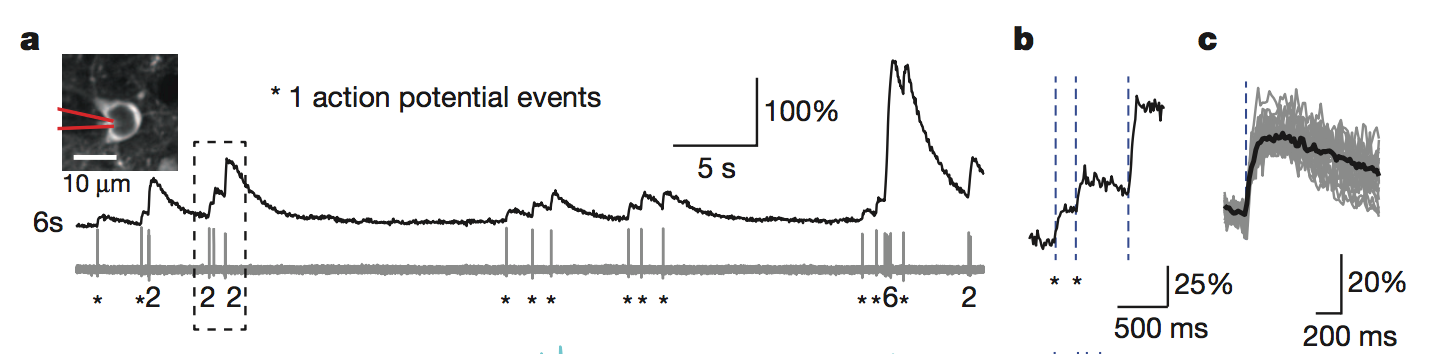
\includegraphics[trim={0 0 0 0},clip,width=0.8\textwidth]{figs/Chen_cai_F3a.png}}
%\subfigure[]{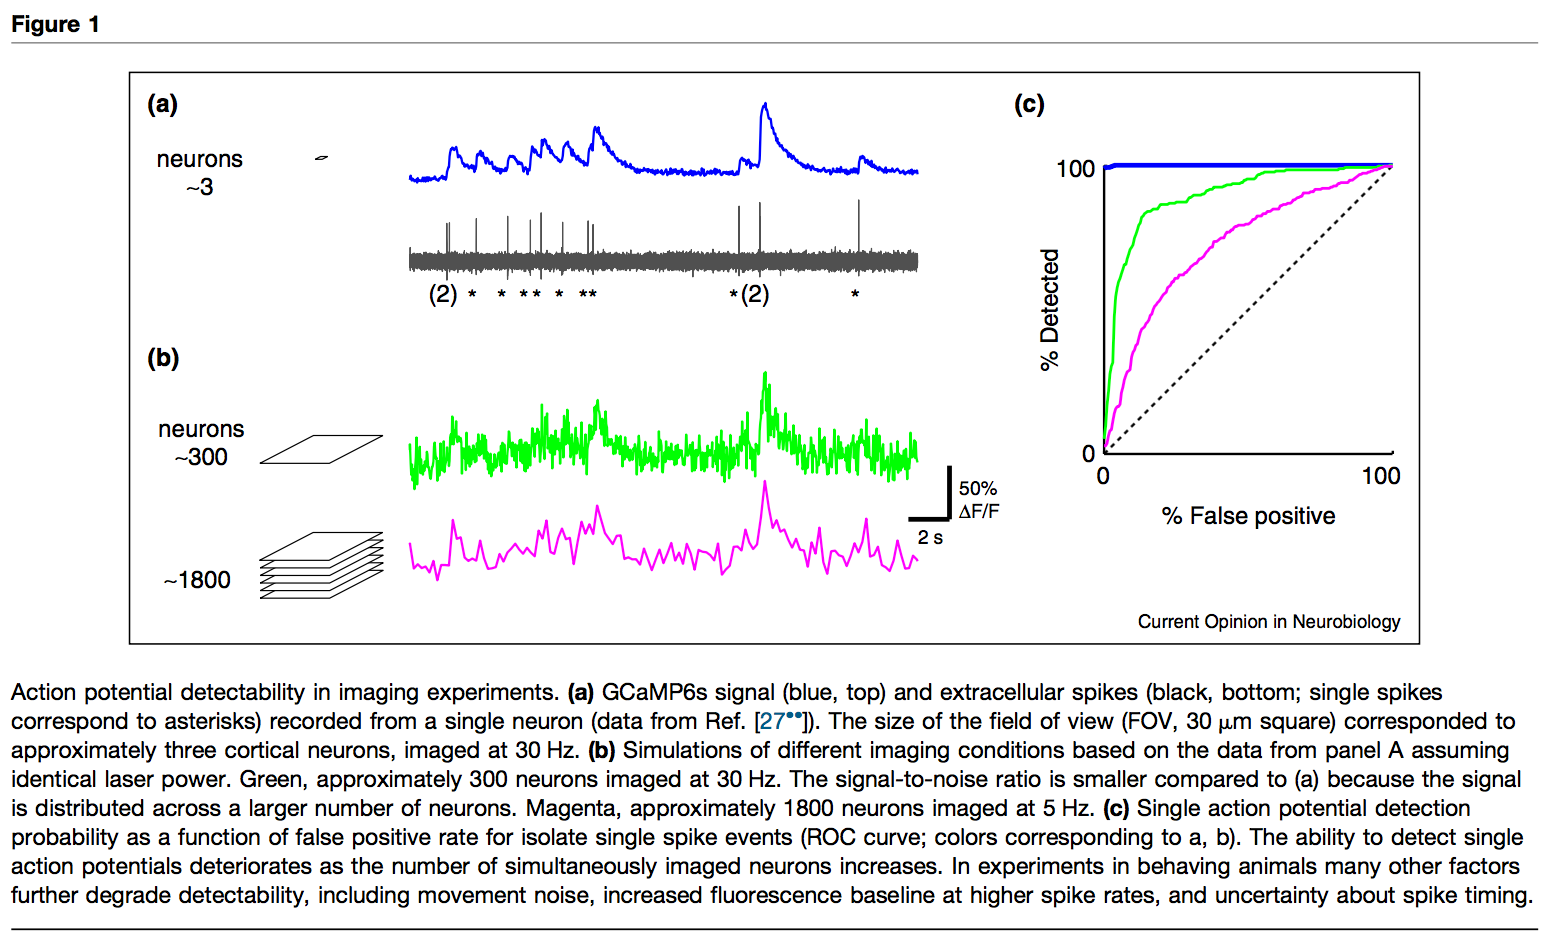
\includegraphics[trim={0 0 0 30},clip,width=0.8\textwidth]{figs/Peron_COiN_15.png}}
%\caption{\label{fig:ground_truth_diagram} (a) Ground truth data collection example from Chen et al. Nature 2013. Top left, an example field of view from imaging data. Red lines denote the outline of a juxtacellular recording pipette. Time series shows measured calcium fluorescence (top) and simultaneously recorded voltage (below). Spikes are marked with asterisks. (b) Frame rate/ spatial resolution trade offs. All light microscopy experiments (including two photon imaging) have a 'photon budget' (set by the microscope and sample) which can be deployed by the experimenters to achieve certain goals. Higher signal to noise can be achieved with high frame rates and zoomed in imaging (more pixels per cell). If the goal is to record from large numbers of neurons the overall photon budget must be spread more thinly per neuron, with smaller numbers of pixels per cell and lower frame rates, resulting in lower signal to noise ratios (Figure reproduced from Peron, Chen \& Svoboda COiN 2015)}
%\end{figure}

\begin{figure*}
\floatbox[{\capbeside\thisfloatsetup{capbesideposition={right,top},capbesidewidth=0.4\textwidth}}]{figure}[\FBwidth]
{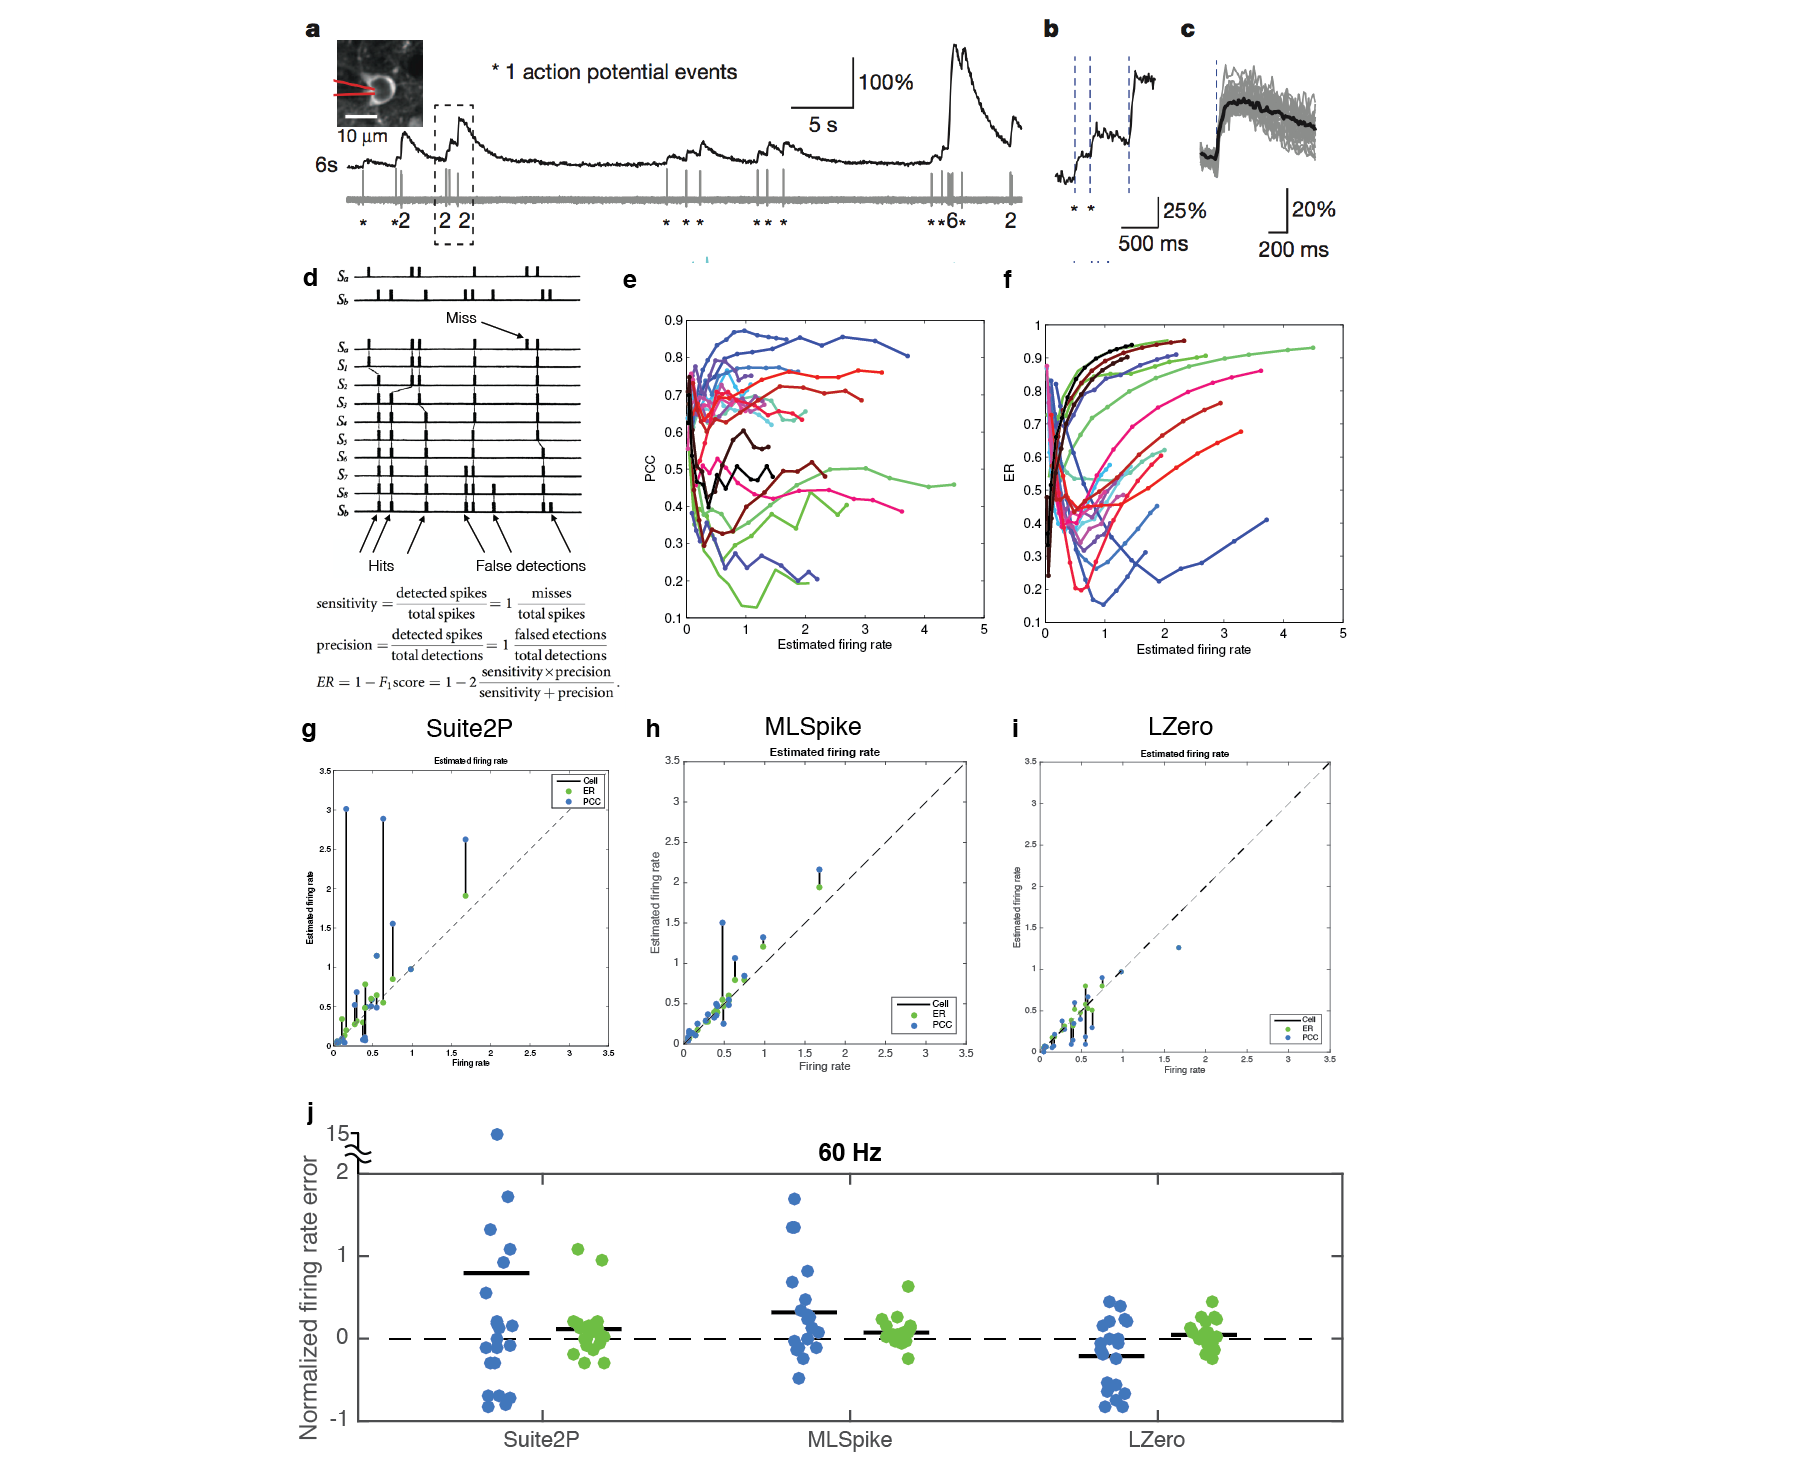
\includegraphics[trim={70 0 110 5},clip,width=0.6\textwidth]{full_figs/why_deconvolve_F1.png}}
{\caption{Ground truth data analysis. (a) Ground truth data collection example from \citet{Chen2013-nv}. Top left, an example field of view from imaging data. Red lines denote the outline of a juxtacellular recording pipette. Time series shows measured calcium fluorescence (top) and simultaneously recorded voltage (below). Spikes are marked with asterisks. (b) Single spikes influence the calcium trace. (c) raw data (grey) and average (black) of single spike induced changes in fluorescence. (d) top: \cite{Victor1996-cg} proposed a spike metric to compare spike trains. This metric is generated by determining the number of elementary operations (shift, addition or deletion of individual spikes - depicted as rows here) required to match two spike trains, up to some temporal precision. Bottom: In \citet{Deneux2016-gu} the Error Rate (ER) is similarly computed as a normalised ratio of sensitivity vs precision in spike detection. Detections are counted to within 0.5s. 
(e) Correlation coefficient as a function of estimated firing rate (using Suite2P, \citet{Pachitariu_undated-ui}). Colours are different cells. (f) as in (e) but with ER as a metric.  (g) Estimated firing rate for `best' deconvolution parameters versus real firing rate. Best parameters are taken as the highest or lowest points in (e) and (f), respectively. (h) as in (g) but using MLSpike \citep{Deneux2016-gu}. (i) as in (g) but using LZero \citep{Jewell2017-pr}. (j) Normalised firing rate error (estimated FR - true FR / true FR) for all cells across all three methods. Lines are means. (a) reproduced from \citet{Chen2013-nv}. (d) reproduced from \citet{Victor1996-cg}. \emph{MDH: Just need to bear in mind that we’ll need a plan for replacing panels a-d with our own plots and schematics}
\label{fig:GT_data}}}
\end{figure*}
%As deconvolution parameters are changed to incrementally increase the estimated firing rate - to trade off hits at the cost of false positive errors - PCC continues to improve (increase) for many cells. In contrast, ER is penalised for overestimating firing rate leading to local minima. Comparing (e) and (f), ER changes smoothly with gradual changes in deconvolution parameters, whereas PCC is more stochastic, leading to noisy estimates of the best parameters.
% PCC both over and underestimates firing rate. ER also overestimates firing rate but to a lesser degree.

\begin{figure*}
\floatbox[{\capbeside\thisfloatsetup{capbesideposition={right,top},capbesidewidth=0.4\textwidth}}]{figure}[\FBwidth]
{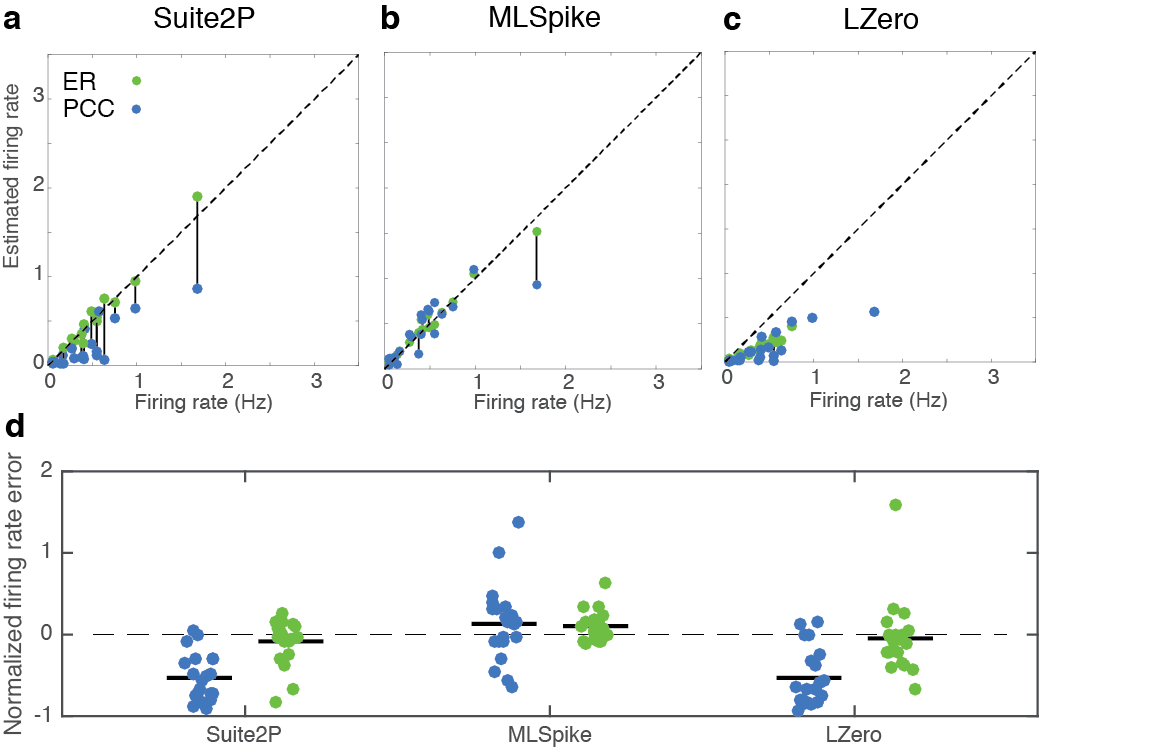
\includegraphics[trim={0 0 25 0},clip,width=0.6\textwidth]{full_figs/why_deconvolve_F1_2.png}}
{\caption{Downsampled ground truth analysis. (a-c) Estimated firing rate for `best' deconvolution parameters versus real firing rate using Suite2P, MLSpike and LZero applied to ground truth data downsampled to 7Hz to more closely match population imaging experiments. (d) Normalised firing rate error (estimated FR - true FR / true FR) for all cells and across methods. Lines are means. 
\label{fig:GT_data_ds}}}
\end{figure*}



\section{Results} 
\subsection{Spike inference methods work well on ground truth data if parameters are fitted using Error Rate instead of Pearson Correlation Coefficient}\label{GT}

%Signposting
%BIG POINT: to check that the spike inference methods can work in principle + benchmark performance with common metrics.
%So we tried three state of the art methods for spike inference on ground truth data.
%
%First. Setting parameters to maximise a common metric (PCC) fails to accurately recover firing rates. This is true across methods, and is no better in the downsampled case.
%
%Second, a different spike-based cost function (ER) leads to good estimates of firing rate across methods, with all methods performing equally well.
%
%Third, good performance results in different parameters across neurons. 
%
%Therefore, what if we use these methods/parameters on real data with no ground truth?



First we assessed the performance of three state-of-the-art spike inference methods under ideal conditions. The methods we tested were Suite2P \citep{Pachitariu_undated-ui},  MLSpike \citep{Deneux2016-gu} and an exact $\ell_{0}$ optimization method (\citet{Jewell2017-pr}, dubbed LZero here). These methods were chosen because of their state-of-the-art performance, difference in underlying algorithm, and open source code. Performance of these methods was evaluated on publicly available ground truth datasets - where the spiking activity of a cell is recorded simultaneously with Ca\textsuperscript{2+} imaging using high-signal-to-noise juxtacellular recording techniques (see Figure \ref{fig:GT_data} (a), \citealp{Chen2013-nv}, \href{https://crcns.org/data-sets/methods/cai-1}{\tt{\color{blue} crcns.org}}). 


% And some idea of what we did would be good: what is the PCC between, and why use it? The PCC is not the thing we’re interested in - it’s the quantity that measures the thing we’re interested in (the apparent quality of recovering spikes from Ca2+ data)
In many spike inference methods papers \citep{Brown2004-tj, Paiva2010-qv,Theis2016-ee, Reynolds2017-dr, Berens2018-su} the metric used to assess performance and optimise model parameters is the Pearson Correlation Coefficient between the true and inferred spike train, due to it's perceived interpretability and wide use in model assessment across neuroscience. Here we determined how correlation coefficient varies with small changes in model parameters, and how it relates to simple measures of neural activity such as firing rate.

% USE ACTIVE VOICE - WE FOUND THAT .... (FIG 1 (e))
Figure \ref{fig:GT_data} (e) shows the results from inferring spikes from ground truth data with Suite2P \citep{Pachitariu_undated-ui} using a range of an internal threshold parameter which trades off misses vs false detections. 

We found that correlation coefficient increases as estimated firing rate increases (Fig. \ref{fig:GT_data}(e)). As a consequence, if we choose the model parameters that maximise the correlation coefficient, the recovered spike-train consistently overestimates the ground truth rate of spiking (Fig \ref{fig:GT_data}(g), blue dots). Over the population, choosing model parameters that optimise correlation coefficient results in over and under estimates firing rate, in some cases by large margins (Figure \ref{fig:GT_data} (g,j), mean error 79.47$\%$ overestimate of firing rate). We found similar results using the two other spike inference methods, with MLSpike and LZero both returning poor estimates of firing rate when optimised using correlation coefficient (Fig \ref{fig:GT_data}(h,i,j), blue dots, mean error 31.72$\%$ overestimates for MLSpike, 21.14$\%$ underestimates for LZero), indicating that it is correlation coefficient and not the methods per se that result in poor performance.

In addition, correlation coefficient does not change smoothly with gradual changes in the threshold parameter, as can be seen in the lines for individual cells in Figure \ref{fig:GT_data} (e), which could lead to overfitting or noisy estimates of the best parameters. 

To address the weaknesses of Pearson correlation coefficient, we implemented the Error Rate (ER) spike distance metric of \citet{Deneux2016-gu}, a summary statistic based on the distance measure of \cite{Victor1996-cg}. ER (outlined in Figure \ref{fig:GT_data} (d)) returns a normalised score which is 0 for a perfect match between two spike trains, and 1 when all the spikes are missed. When evaluating the same inferred spike trains from \ref{fig:GT_data}(e), ER is best (lowest) for intermediate estimated firing rates, suggesting that estimates closer to the true firing rate are rewarded with good scores (Figure \ref{fig:GT_data} (f)). In addition, unlike for correlation coefficient, individual cell results in Figure \ref{fig:GT_data} (f) show ER varies smoothly with gradual changes in Suite2P's threshold parameter. 

%This intuition is shown to be true when comparing the best estimate of firing rate to the true firing rate for each cell (green dots in Figure \ref{fig:GT_data} (g, j left)). 

Across all three spike inference methods, optimising parameters with ER results in much better estimates of firing rate compared to optimisation with correlation coefficient  (mean error <10$\%$ - 0.12$\%$ Suite2P, 0.073$\%$ MLSpike, 0.05$\%$ LZero, compare blue and green dots in \ref{fig:GT_data} (g-j)). 
%ER results in better estimates of firing rate than correlation coefficient when it is used to optimise parameters for the two other spike inference methods tested, MLSpike (Fig \ref{fig:GT_data} (h, j middle)) and LZero (Fig \ref{fig:GT_data} (i, j right)). 
In sum, our results show that three different spike inference methods can accurately recover firing rate if Error Rate is used to optimise model parameters on ground truth data instead of correlation coefficient. 

%\emph{MDH: As we are making a comparison between PCC and ER here, we should group the results for the three algorithms. 
%So figure 1e illustrates the problem with PCC for Suite2P; and figures 1g-l show that using “optimal” PCC gives errors in estimating firing rates for all three algorithms. Naively suggests algorithms are crap.
%Thus we try ER instead to tune the algorithms’ parameters. And now we see (Figs 1f-l) that all three algorithms can accurately recover the spike rate of the ground truth neurons. 
%But, final check - low frame rate...}

%(1) does a lower frame-rate improve the ability of PCC to recover ground-truth?
%(2) does a lower frame-rate worsen the ability of ER to recover ground-truth?

All light microscopy experiments (including two photon imaging) have a `photon budget' (set by the microscope and sample) which can be deployed by the experimenters to achieve certain goals. Higher signal to noise can be achieved with high frame rates and zoomed in imaging (more pixels per cell), as is the case for the ground truth datasets analysed here (60Hz imaging). If the goal is to record from large numbers of neurons the overall photon budget must be spread more thinly per neuron, with smaller numbers of pixels per cell and lower frame rates, resulting in lower signal to noise ratios \citep{Peron2015-qz}. %Large scale Ca\textsuperscript{2+} imaging experiments are optimised to record from many neurons at once, and typically use lower frame rates and fewer pixels per cell than the ground truth experiments described above. 
Given that the ground truth dataset described above was recorded at 60Hz, it is important to ask whether imaging at a lower frame rate improves the ability of Pearson correlation coefficient to recover ground truth spiking, and whether lower frame rates impair the ability of Error Rate to recover accurate spiking estimates.

To assess the effect of sampling rate on spike inference we repeated the ground truth analysis, but with imaging data down-sampled to 7Hz and found similar results to the 60Hz case. Optimising spike inference parameters with Error-Rate leads to better estimates of firing rate than optimising with correlation-coefficient (Fig \ref{fig:GT_data_ds}, mean absolute error 39.7$\%$ (-53.0,13.3,-52.9) for correlation coefficient, 7.8$\%$ (-8.3,10.4,-4.7) for Error Rate). Interestingly, optimising with correlation coefficient leads to underestimates of firing rate at 7Hz (Fig \ref{fig:GT_data_ds} (d)), where overestimation is more typical with 60Hz data (Fig \ref{fig:GT_data}).


One goal of ground truth analysis is to find optimal analysis parameters for experiments where ground truth is not available. Figure \ref{fig:GT_data_params} shows the best parameters for each cell across spike inference methods and sampling rates. Across all conditions, there is substantial variability across cells, with best parameters varying over two orders of magnitude in some cases (left hand panels of Fig. \ref{fig:GT_data_params}). This suggests that the best parameters for one cell may perform poorly for another cell, and optimising spike inference parameters in the absence of ground truth data may be difficult.

\begin{figure}[h!]
{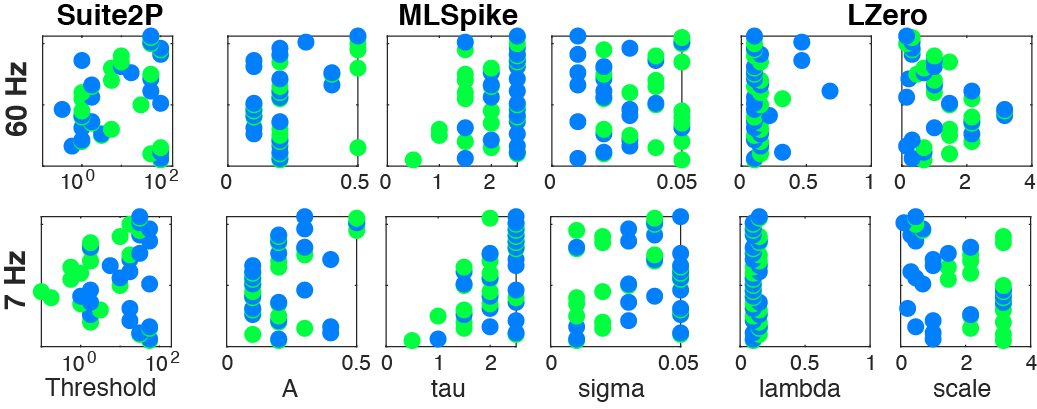
\includegraphics[width=\textwidth]{full_figs/why_deconvolve_F1_3.png}}
{\caption{Best spike inference parameters varies across cells. X-axis: parameter value, Y-axis: cell ID (arbitrary but consistent order). Parameters for Suite2P (Threshold), MLSpike (A, tau, sigma) and LZero (lambda, scale) vary significantly across cells and sampling rates (rows), regardless of analysis metric (dot colour, ER: green, PCC: blue).
\label{fig:GT_data_params}}}
\end{figure}

To further illustrate this point we analyzed how firing rate estimates and Error Rate vary with deviations from the best analysis parameters (for Suite2P applied to downsampled data, as in Fig.\ref{fig:GT_data_ds}).  Fig. \ref{fig:GT_param_performance} (a) shows estimated firing rate departs from the true firing across a range of analysis parameters. Normalizing the results by each cell's true firing rate (Fig. \ref{fig:GT_param_performance} (b)) show that firing rate errors are particularly large for low firing rate neurons - a particular concern for applications of spike inference to data from cortex in awake animals where low firing rates are the norm \citep{OConnor2010-hd,Wohrer2013-rp}. Fig.\ref{fig:GT_param_performance} (c) shows how Error Rate changes as parameters are varied from the best parameters in Fig.\ref{fig:GT_data_ds}. Error Rate increases abruptly with small increases or decreases in the best parameters. Fig.\ref{fig:GT_param_performance} (d) shows the same data as in (c) but for a restricted range of analysis parameters, emphasising how Error Rate can increase with even very small changes in analysis parameters.

\begin{figure}[h!]
{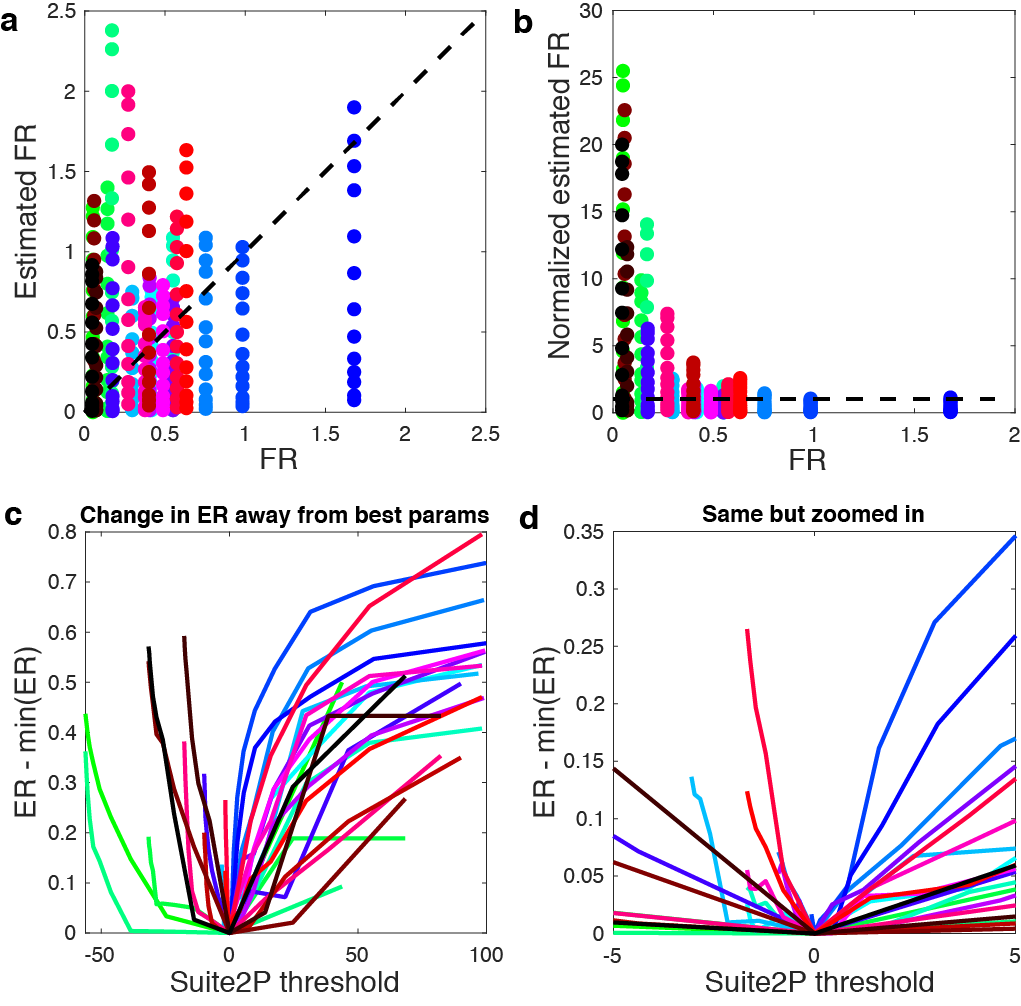
\includegraphics[width=\textwidth]{full_figs/why_deconvolve_F1_4_colours.png}}
{\caption{Variability in spike inference performance with changes in analysis parameters. (a) For each cell (colours) the estimated firing rate (y-axis) varies substantially across analysis parameters (dots). Dashed black line indicates correct estimated firing rate. (b) as in (a) for normalized estimated firing rate (Estimated FR/true FR). (c) Error rate increases sharply with small changes away from the best analysis parameters. (d) as in (c) showing a small region of parameter space around the best parameters). All results are from Suite2P applied to downsampled data as in Fig.\ref{fig:GT_data_ds}.
\label{fig:GT_param_performance}}}
\end{figure}

Together, these results show that modern spike-inference methods can accurately recover neural activity, but the choice of metric for evaluation and fitting of parameters are of critical importance. Pearson correlation coefficient is a poor choice of metric as it returns inconsistent results with small changes in algorithm parameters, and leads to poor estimates of simple measures such as firing rate when used across methods and sampling rates. A spike-train-based method such as Error Rate\citep{Deneux2016-gu, Victor1996-cg}, or other recently developed methods based on information theory \citep{Theis2016-ee} or fuzzy set theory \citep{Reynolds2017-dr}, are more appropriate. However, while good estimates of neural activity can be achieved with modern spike inference methods the best parameters vary substantially between cells, and small changes in analysis parameters result in poor spike inference performance. This suggests spike inference may not be successful when ground truth data is not available, and parameters cannot be optimised for each cell.
%Reynolds - a continuous approach based on fuzzy set theory. Theis - information gain.

%\clearpage
\subsection{Spike inference and deconvolution methods disagree on estimates of simple neural statistics}
%\noindent \emph{\textbf{Results in brief}\\
%- we want to see what effect deconvolution/spike inference method choice has on data analysis\\
%- methods (within and between 'class' i.e. deconvolution vs spike inference) disagree on event rate of cells
%- some methods are qualitatively wrong, others have quantitative disagreement\\
%}
\begin{figure}[h!]
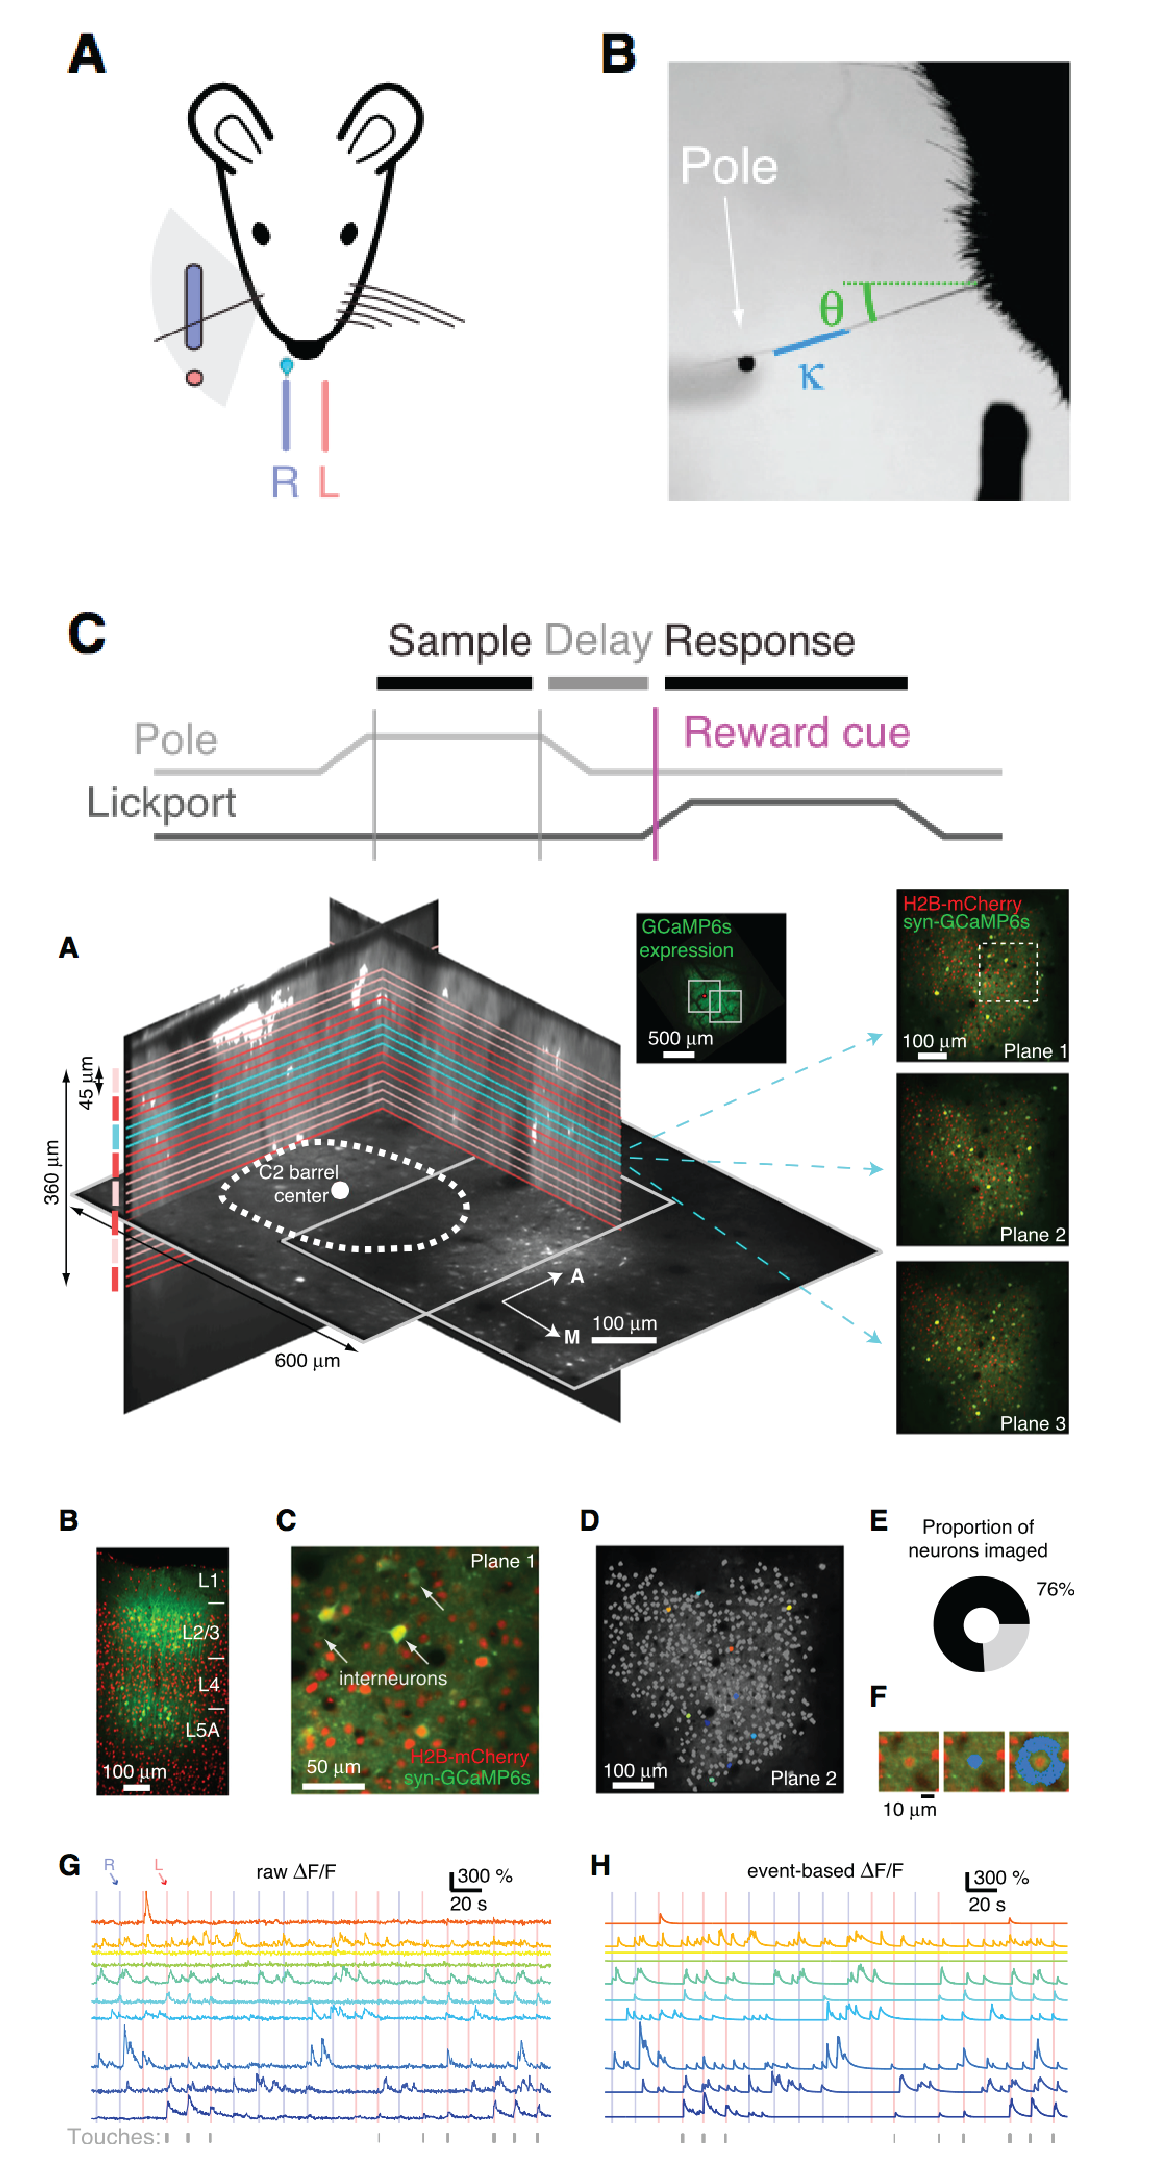
\includegraphics[width=0.9\textwidth]{full_figs/why_deconvolve_F2.png}
\caption{\label{fig:peron_setup} \citep{Peron2015-qz} experimental design. TO DO EXPAND description once final figure arrangement is decided 
\emph{MDH: Again, we need to think about how to remove or replace these figure panels for publication.
We don’t need  the bottom rows of A-F here for example. For our purposes, we only care that there is a single recording of many neurons during a task.
So versions of the bottom row G and H from the actual session we use would be good for the final version.
We can redraw the top row A and C; 
For the parameters in top panel B, as far as I know these aren’t used here (just “touch”), so an be eliminated too. If we need them, then the redrawn A panel can have the angle and curvature parameters from B}}
\end{figure}

We have shown that different spike inference methods can recover good estimates of neural activity if parameters are set appropriately. However, it is not possible to fit parameters to representative ground truth data for most experiments. On a real-world example, does spike inference result in good estimates of neural activity, and how do these estimates compare to simple deconvolution or de-noising processes? 

To determine the effect of analysis method and parameter choice on simple measures of neuron activity in the absence of ground truth, we compared the results of analysis of df/f Ca\textsuperscript{2+}  from a single experiment from \citealt{Peron2015-qz} (see Figure \ref{fig:peron_setup}) to eight different approaches for deconvolution, de-noising and spike inference. We compared the three spike inference methods tested in Section \ref{GT} - Suite2P, MLSpike and LZero - to a kernel-convolved version of the returned spikes (i.e. denoised df/f); de-noised Ca\textsuperscript{2+} as reported in the original \citet{Peron2015-qz} study; and the simple deconvolution approach of \citet{Yaksi2006-ic} (see Methods for implementation details).

%\emph{We’ll need to explain the collection of algorithms here, including why we’re expanding from the original 3. (Spike inference vs plain deconvolution to understand if we gain anything; and compare all to raw Ca2+)}

%trim={0 85 40 80},clip,
\begin{figure*}
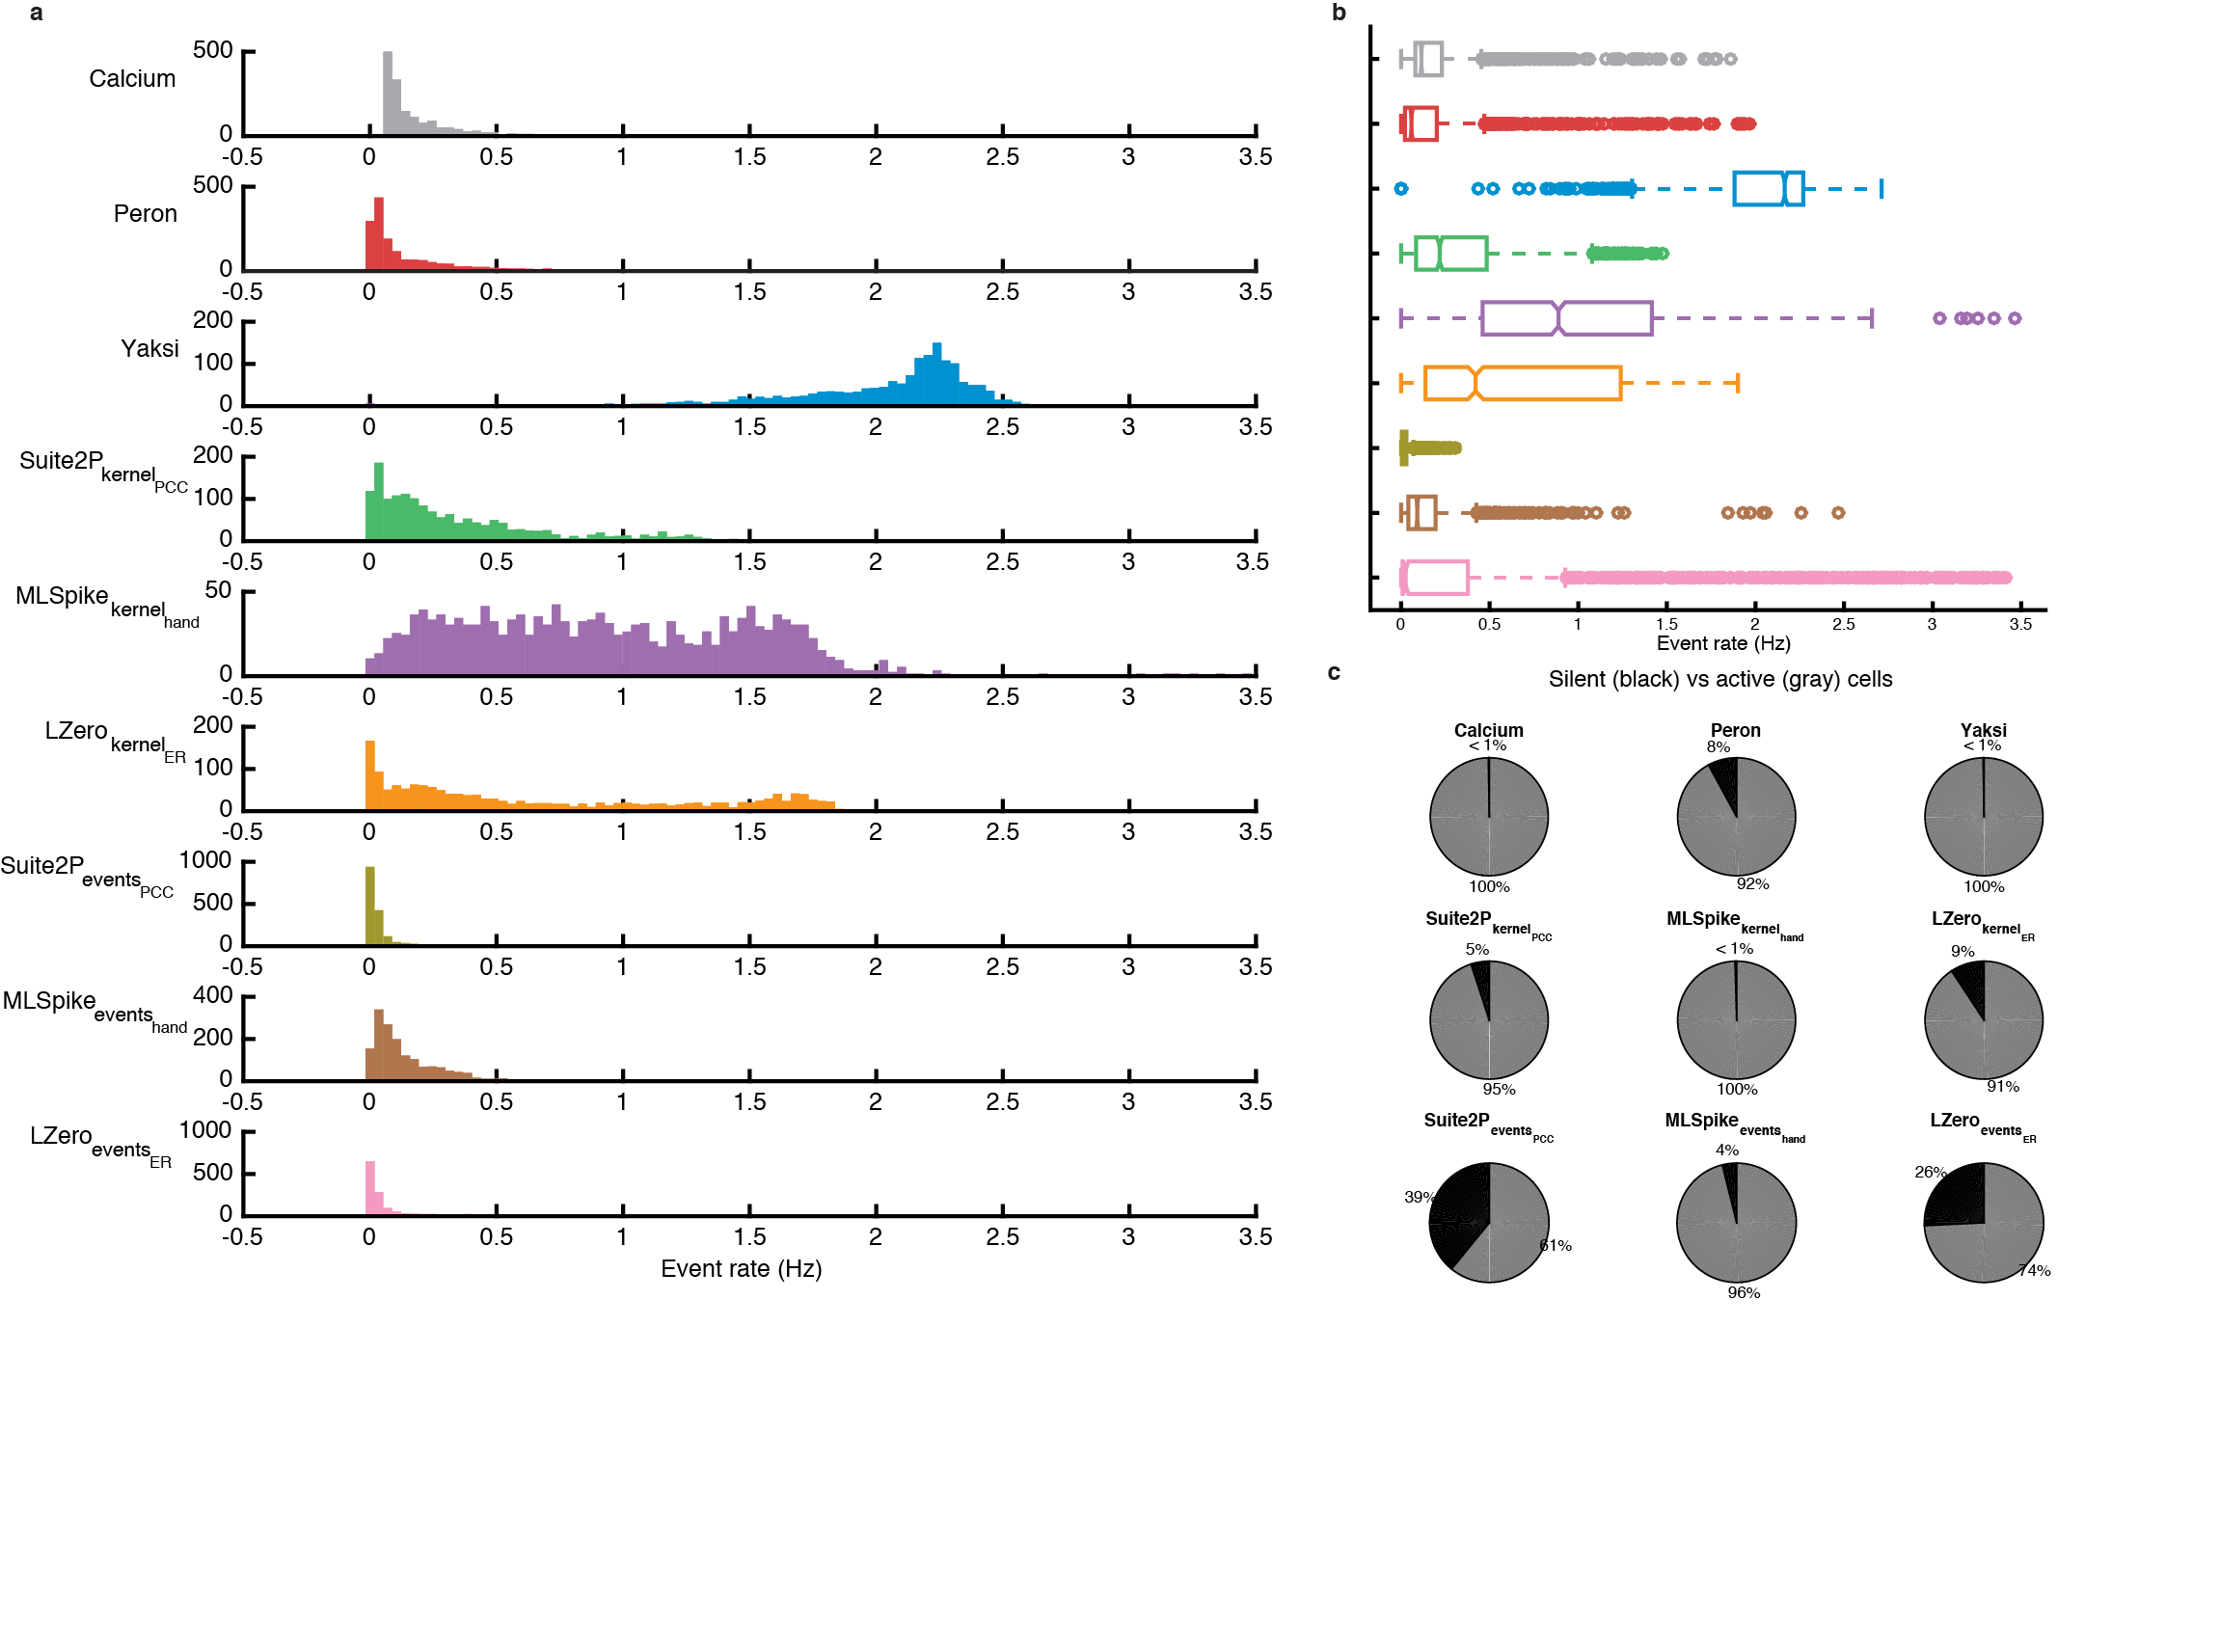
\includegraphics[trim={0 85 40 0},clip,width=\textwidth]{full_figs/why_deconvolve_F3_3.png}
\caption{\label{fig:simple_stats} Estimated `event rate' for all cells in an example session. For the first 6 methods (Calcium - LZero$_{kernel}$), events are detected as fluorescence transients greater in magnitude than 3 std deviations of background noise. Background noise = data - smoothed version of data, to eliminate slow transients. Methods 7-9 (Suite2P$_{events}$ - LZero$_{events}$) return a spike count per time bin. (a) Histograms of event rate per cell for each method. (b) Same data as in (a) but plotted as box and whisker plots. Notch = median, box limits = 25th and 75th percentile, whiskers = extent of data up to 1.5 IQR (c) Proportion of active (gray) vs silent (black) cells for each method. Silent = event rate < 0.0083Hz.}
\end{figure*}

In \citealt{Peron2015-qz} two-photon Ca\textsuperscript{2+} imaging was used to record neural activity from up to $\sim$2000 neurons simultaneously at 7Hz from superficial barrel (Layer 2/3 somatosensory) cortex as mice performed a head-fixed tactile localisation task with their whiskers. For the results presented here 1552 neurons were recorded for a total of just over 56 minutes (23559 time points). This relatively long recording ensured good estimation of the measured parameters (e.g. pairwise correlations are stable, see Fig. \ref{fig:supp_cxy_stability}).


%\begin{figure}[h!]
%\centering
%\subfigure[]{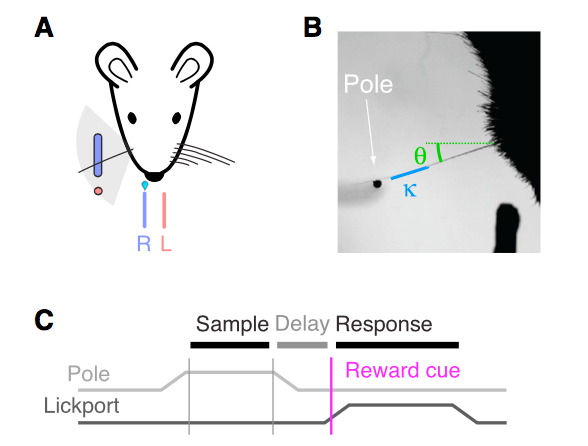
\includegraphics[trim={0 0 0 0},clip,width=0.4\textwidth]{figs/Peron_F1.png}}%
%\subfigure[]{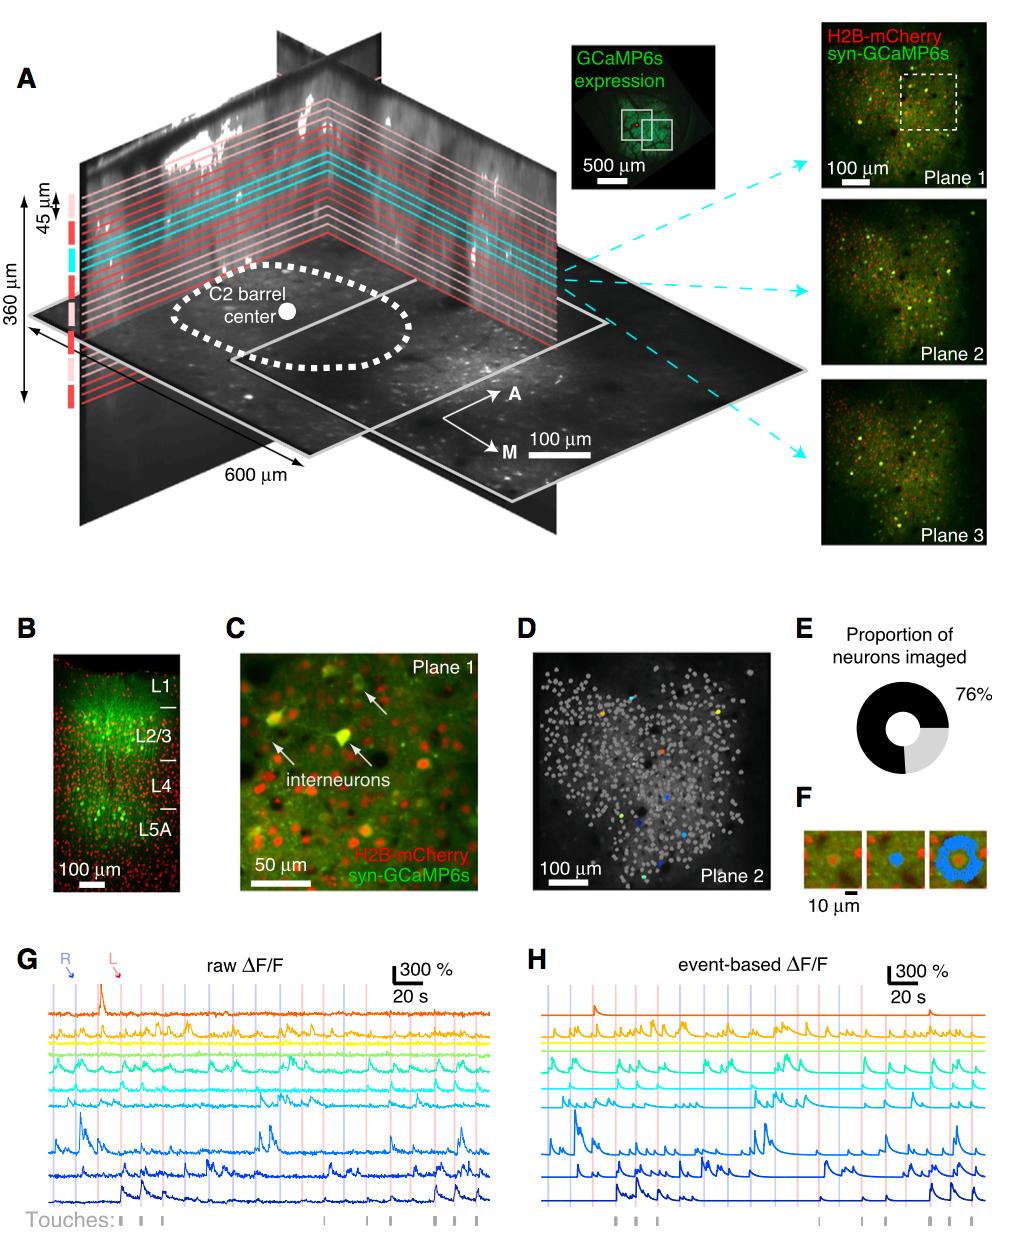
\includegraphics[trim={0 0 0 0},clip,width=0.4\textwidth]{figs/Peron_F2.png}}
%\caption{\label{fig:peron_setup} Peron et al. 2015 experimental design. TO DO EXPAND description}
%\end{figure}

The most basic analysis of neural activity is to determine the mean firing rate of each cell in the recording - a quantity that is known to follow an approximately log normal distribution at the population level \citep{Wohrer2013-rp}. We determined the mean spike/event rate per cell for all approaches (see Methods). Figure \ref{fig:simple_stats} (a) and (b) show that no two methods return the same distribution of spike/event rates. The deconvolution methods (Yaksi - LZero$_{kernel}$) appear to overestimate the average firing rate of the population as well as the number of cells with high firing rates. Spike inference methods can be tuned to produce qualitatively correct distributions (median near zero, long right skewed tails), but they disagree quantitatively. 

% \textbf{TO DO: Add back in 'straw man' results based on best ground truth parameters?}. \emph{Need to clarify 'hand tuning' and put the GT derived params first, then hand tuned results}.

It has been estimated from cell-attached recordings that $\sim$13\% of somatosensory neocortical cells are silent during the pole localisation task (fewer than one spike every two minutes, \citealt{OConnor2010-hd}), a quantity increasing to $\sim$26\% in Layer 2/3. For the nine approaches we tested, in seven the estimated proportion of silent cells to be below 10\%, with wide disagreement between the other two methods (Figure \ref{fig:simple_stats} (c)). Even for simple statistics, the choice of deconvolution or spike inference method results in widely different results.

%\begin{figure}%[h!]
%\centering
%\subfigure[]{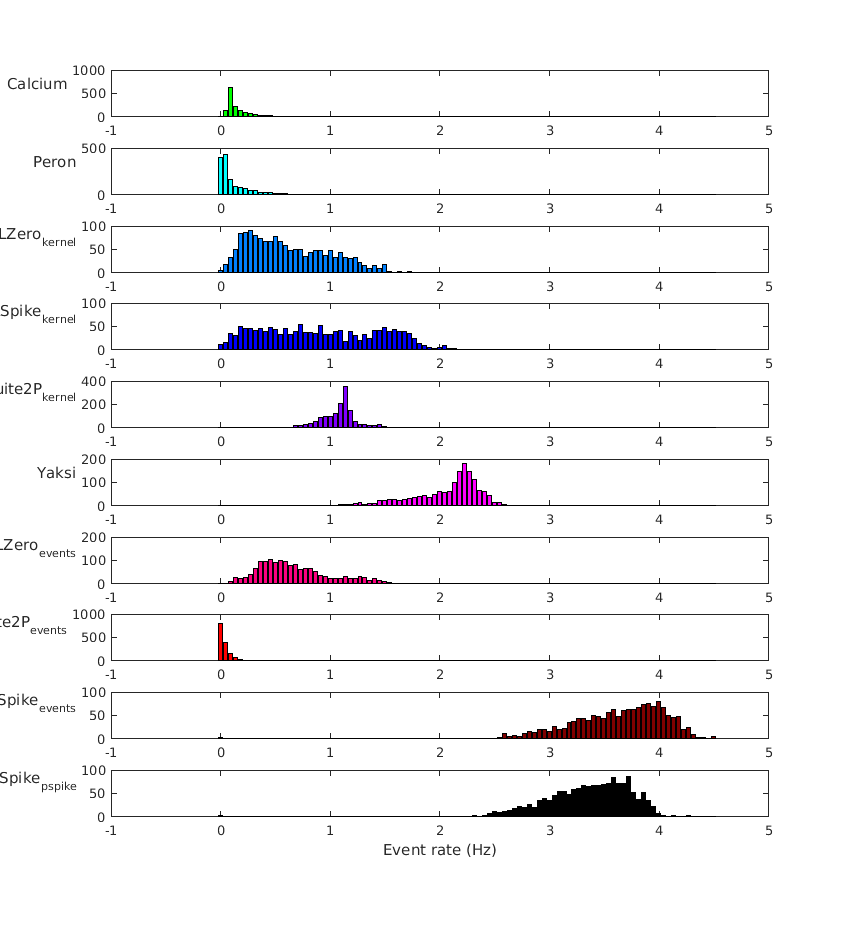
\includegraphics[trim={0 20 50 25},clip,width=0.5\textwidth]{figs/event_rate_all.png}}
%\subfigure[]{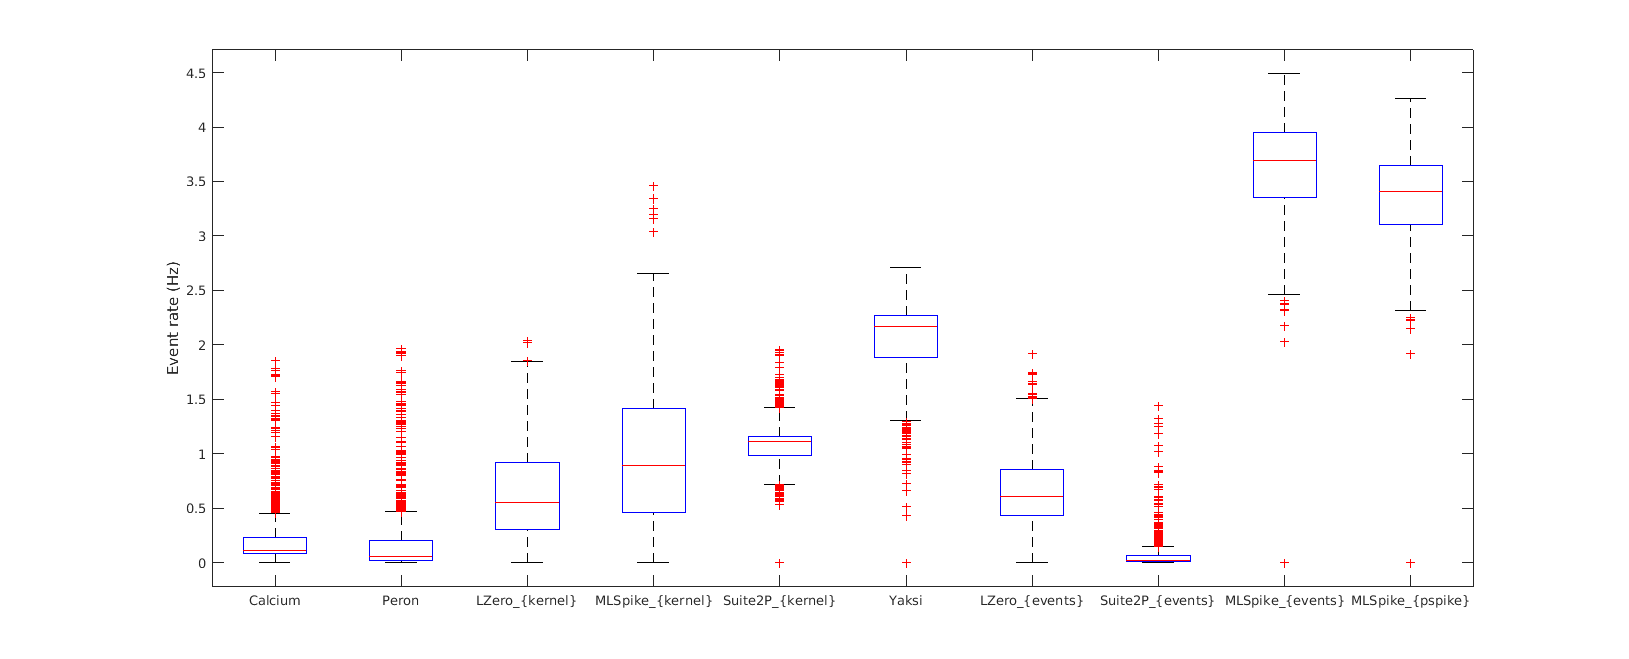
\includegraphics[trim={100 20 110 25},clip,width=0.5\textwidth]{figs/event_rate_dist_all.png}}
%\subfigure[]{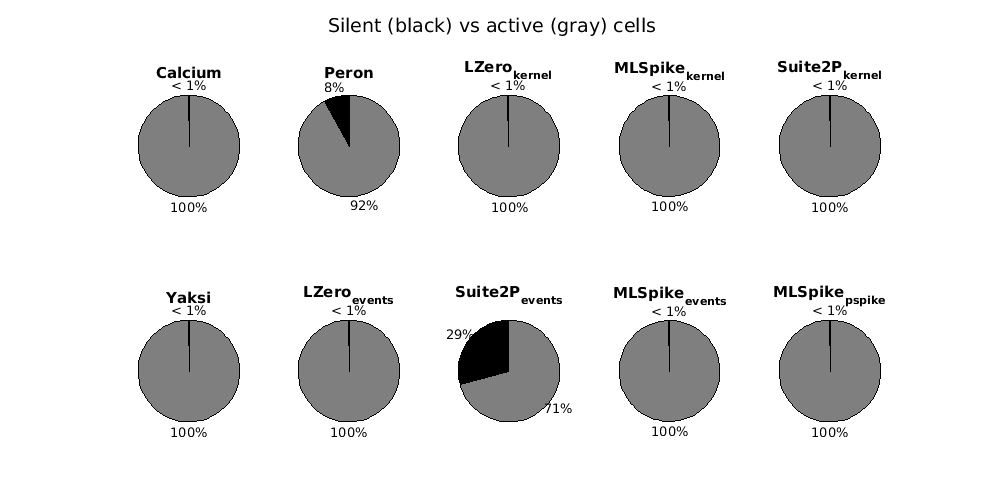
\includegraphics[trim={80 30 60 10},clip,width=0.5\textwidth]{figs/silent_cells_all.png}}
%\caption{\label{fig:event_detection} Estimated 'event rate' for all cells in an example session. For the first 6 methods (Calcium - Yaksi), events are detected as fluorescence transients greater in magnitude than 3 std deviations of background noise. Background noise = data - smoothed version of data, to eliminate slow transients. Methods 7-10 (LZero$_{events}$ - MLSpike$_{pspike}$) return a spike count per time bin. (a) Boxplots of event rate per cell for each method. (b) Same data as in (a) but plotted as box and whisker plots. (c) Proportion of active (gray) vs silent (black) cells for each method. Silent = event rate < 0.0083Hz.}
%\end{figure}




%\newpage



%\clearpage
\subsection{Different spike inference methods lead to different estimates of task related neurons}
%\noindent \emph{\textbf{Results in brief}\\
%- Absolute firing rate may not be important, so what about task related activity?\\
%- Different methods disagree about the number of task-tuned cells\\
%- Different methods disagree on the identity of task-tuned cells\\
%- Cells classed as tuned by one method lacks clear task related activity when processed with another method\\
%- This disagreement means either (a) some tuned cells are missed (b) some un-tuned cells are classed as tuned (c) both.\\
%- Spike inference/ deconvolution leads to fewer neurons classified as task tuned (vs calcium), perhaps due to removal of task-related changes\\
%- Agreement between methods may be an indicator of robust tuning\\
%}


For many analyses, it is the relative activity of a cell and not its exact firing rate that is important. A common analysis is to ask whether a neuron's activity is task related - does a cell respond more during a specific epoch of the task than would be expected from a random process. Such task tuning may then imply that a given cell or region of the brain is involved in the task, and serve as a target for future causal or manipulation studies. We quantified the proportion of task related neurons in our dataset following the approach of \citealt{Peron2015-qz}. Calcium/instantaneous firing rate/ events for each cell are shuffled in time before a trial-averaged PSTH is generated, and the largest peak in the PSTH is recorded. This is repeated 10,000 times. 


\begin{figure}
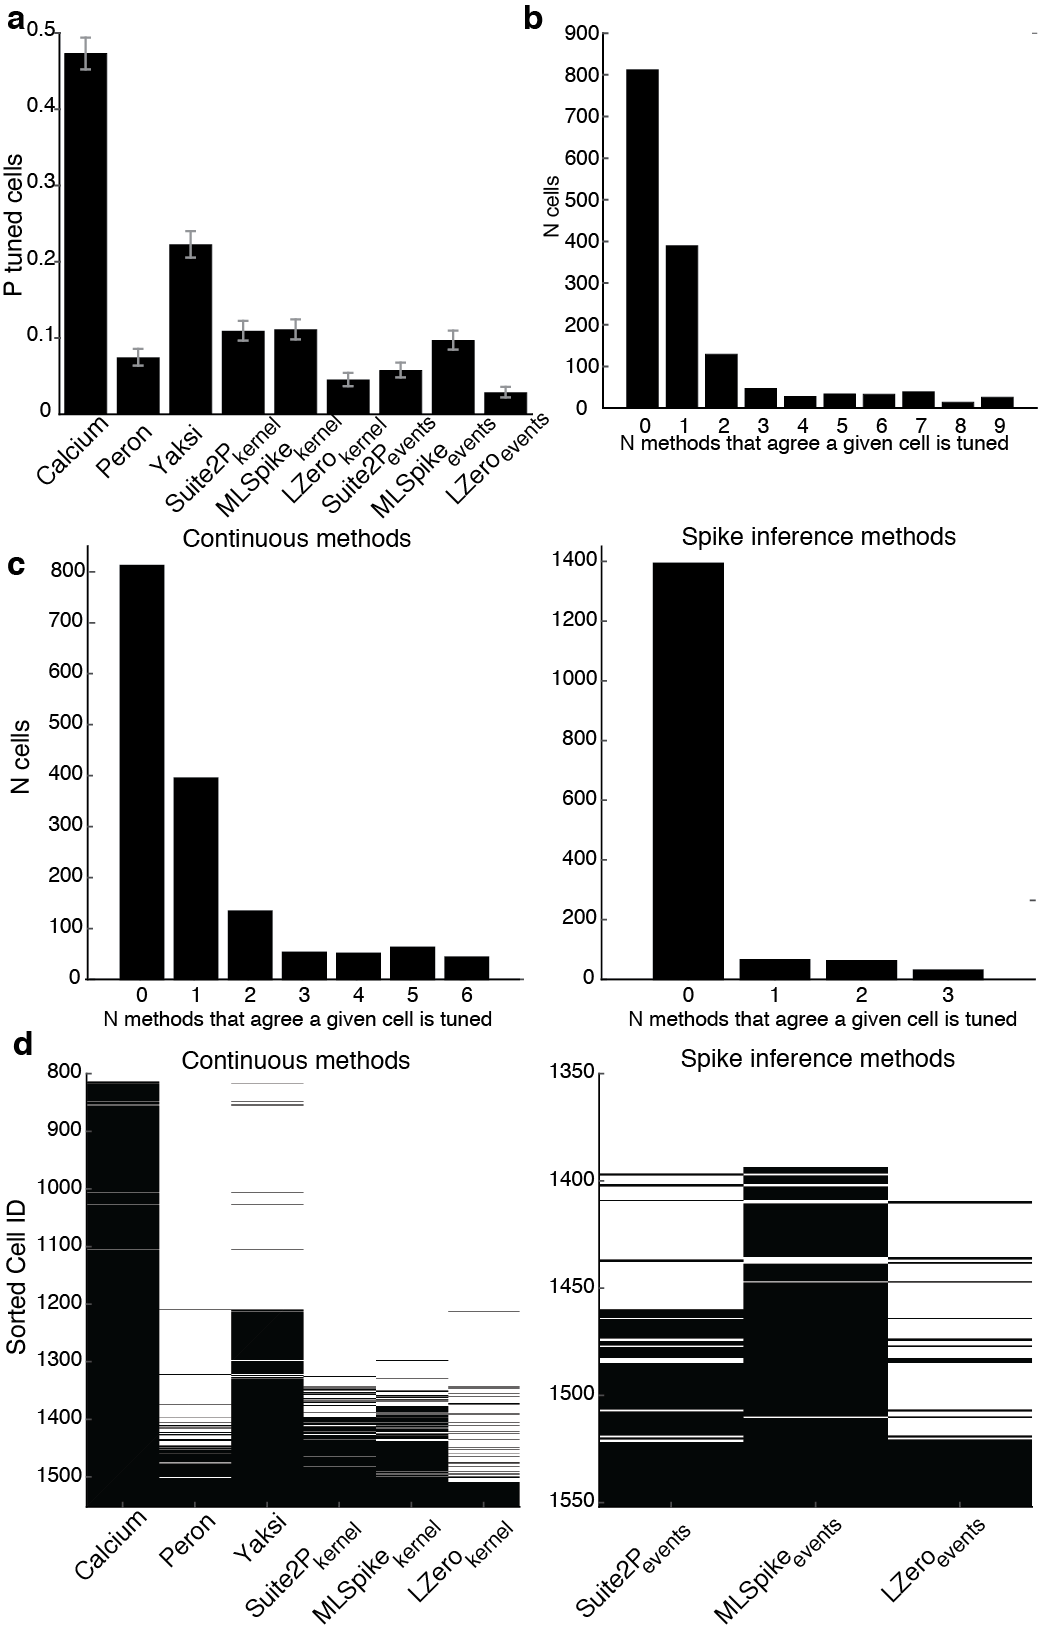
\includegraphics[trim={0 0 0 0},clip,width=\textwidth]{full_figs/why_deconvolve_F4_3.png}
\caption{\label{fig:tuned_cells} Tuned cells. Tuned cells were determined through shuffle tests (following Peron et al 2015, see Methods).  (a) Number of tuned cells per deconvolution method. Error bars are 95\% binomial confidence intervals (Jeffreys interval) (b) Agreement between methods. Bars show total number of cells classified as tuned by N methods. (c) Agreement between continuous signal methods (left) and spike inference methods (right). (d) Array of tuned cell identities, separately for continuous signal methods (left) and spike inference methods (right). Black = tuned, white = not tuned. Rows are cells, ordered by the number of methods that classify that cell as tuned (agreement, as plotted in c).}
\end{figure}

A distribution of shuffled PSTH peak magnitudes is generated, and if the peak of the true (data) PSTH is larger than the 95\%ile of the shuffled distribution, in either the Left or Right (Go, No Go) trials, that cell is considered `tuned'.
Firstly, each method estimates a different proportion of tuned vs untuned cells, both in comparison to estimates from the raw Ca\textsuperscript{2+}, and in comparison to one another (Fig. \ref{fig:tuned_cells} (a)). Secondly, the methods only agree on the tuned status of individual neurons for $<$50 cells (from a range of 50 - 250 tuned cells Fig. \ref{fig:tuned_cells} (b)). \textbf{TO DO get precise number?}. 

There is still substantial disagreement when comparing methods within class: whether looking at deconvolution and de-noising methods (Fig. \ref{fig:tuned_cells} (e), left) or spike inference methods (Fig. \ref{fig:tuned_cells} (e), right), all methods only agree on the tuned status of $<$ 50 cells. This result is problematic, as this disagreement could mean either (a) some tuned cells are missed (b) some un-tuned cells are classed as tuned (c) both. Looking at each cell's tuned status in more detail (Fig. \ref{fig:tuned_cells} (d)) it becomes clear that while some cells are only classified as tuned by one or two methods, there is wider agreement between methods about a larger group of cells \textbf{TO DO get proportion}, suggesting agreement between methods may a robust cue to tuning.

%There is substantial disagreement between methods.

%\textbf{TO DO: compute PSTH for tuned vs untuned cells. This may be the time to look at Yaksi $\&$ Friedrich style temporal correlations...}

%\begin{figure}
%\centering
%\subfigure[]{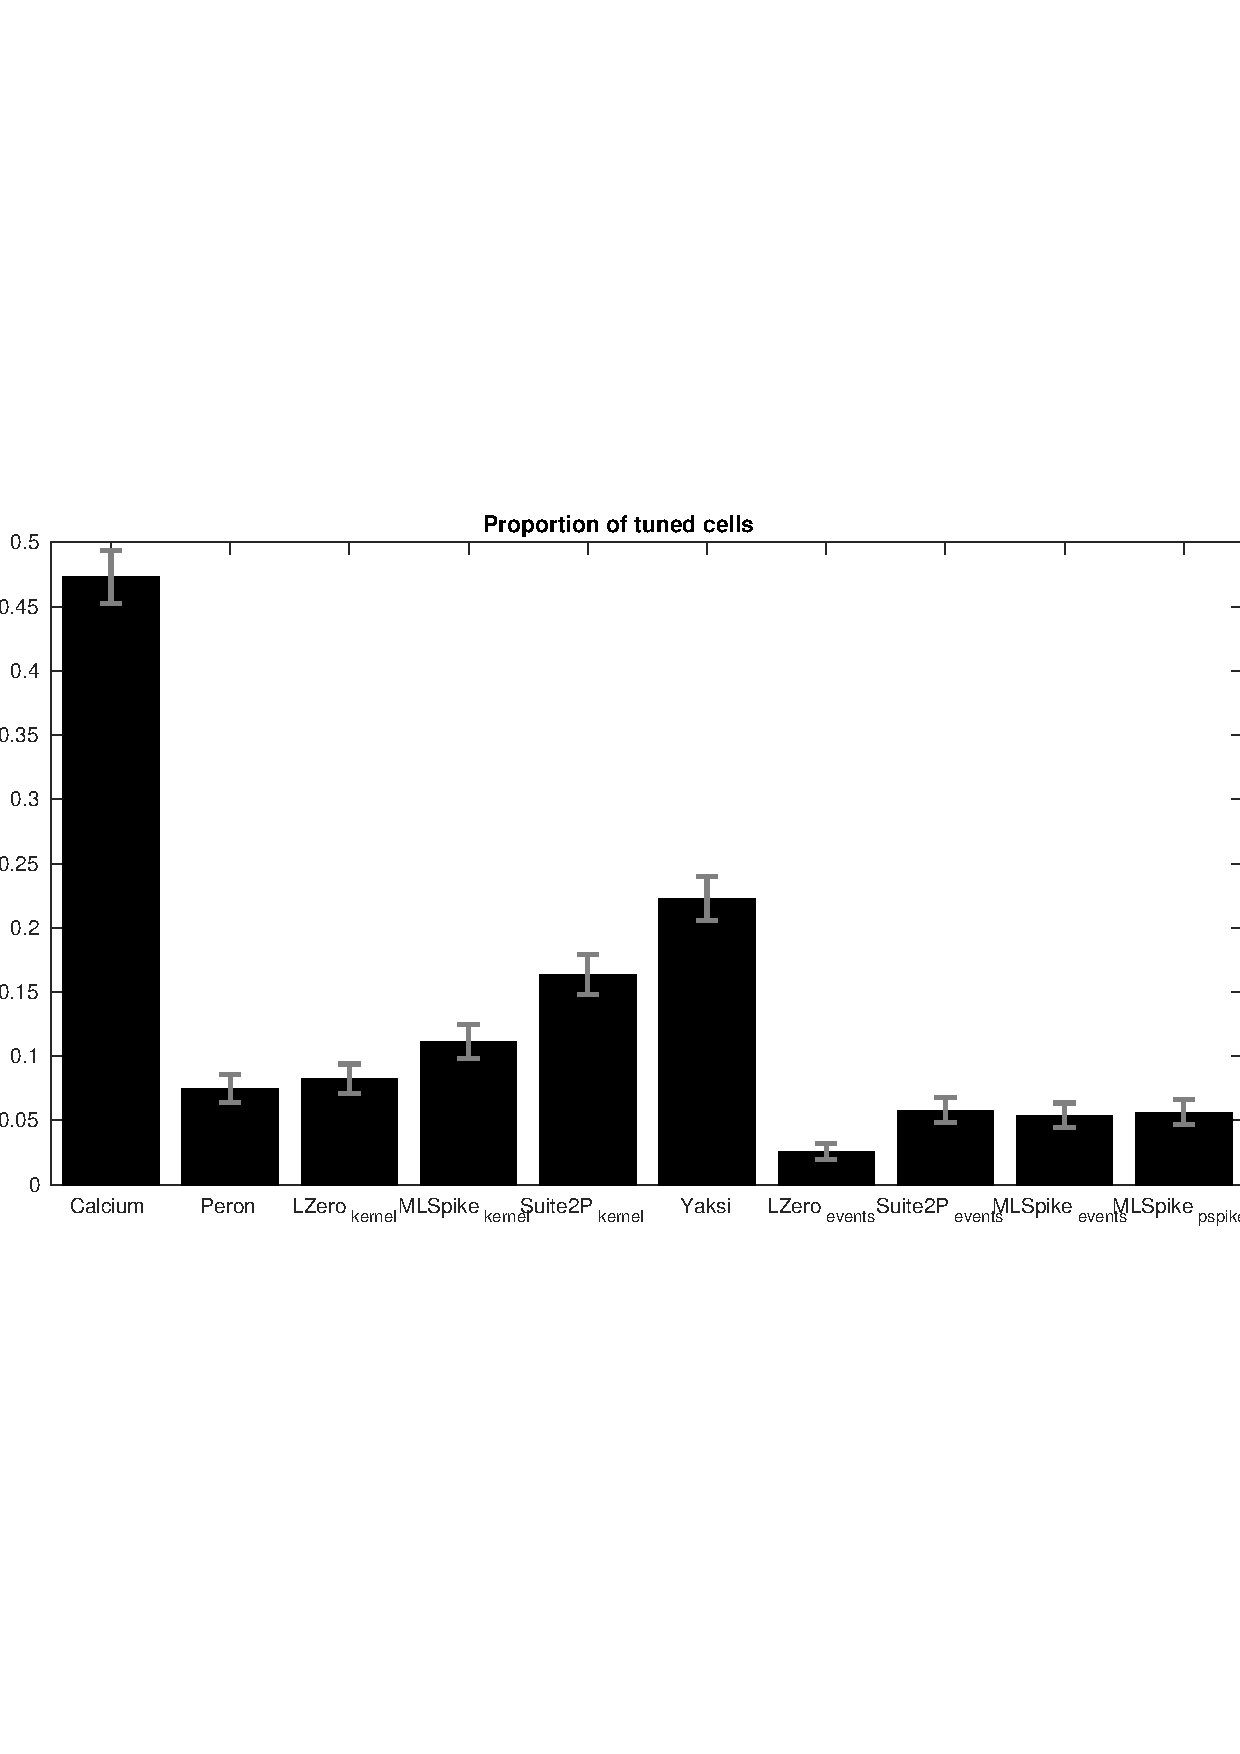
\includegraphics[trim={0 250 0 240},clip,width=0.7\textwidth]{figs/Tuned_cell_all_zoom.pdf}}
%\subfigure[]{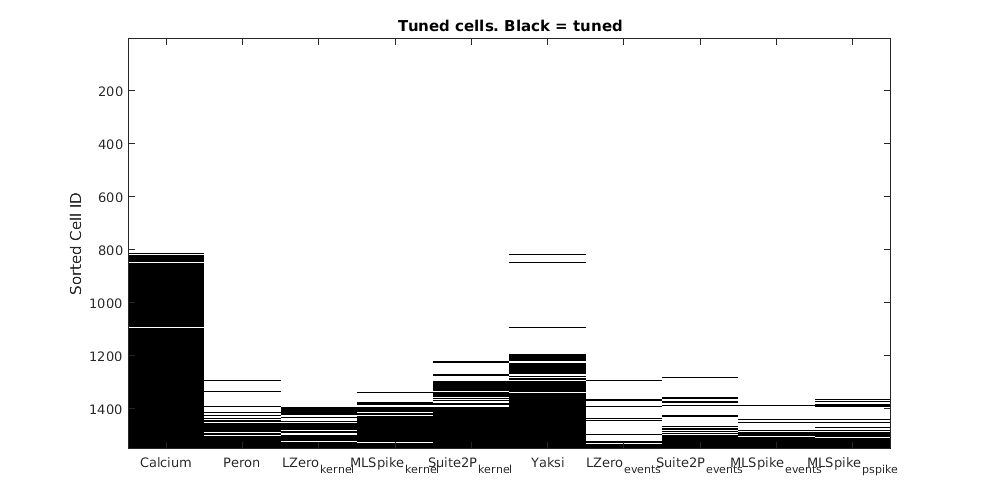
\includegraphics[trim={50 25 60 10},clip,width=0.7\textwidth]{figs/tuned_array2.png}}
%\subfigure[]{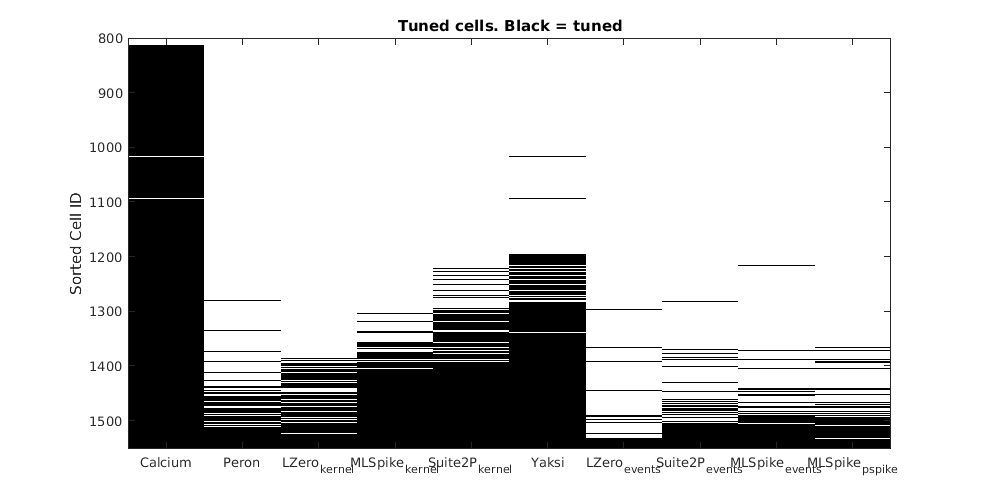
\includegraphics[trim={50 25 60 10},clip,width=0.7\textwidth]{figs/tuned_array2_zoom.png}}
%\caption{\label{fig:tuned_cells} Tuned cells. Tuned cells were determined through shuffle tests (see main text).  (a) Number of tuned cells per deconvolution method. Error bars are 95\% binomial confidence intervals (Jeffreys interval) (b) Array of tuned cell identities. Black = tuned, white = not tuned. Rows are cells, ordered by the number of methods that classify that cell as tuned. (c) Zoomed in version of (b). There is substantial disagreement between methods.}
%\end{figure}

Figure \ref{fig:tuned_cells_psth} shows the trial-averaged activity for cells classified as tuned when looking at raw Calcium data only (Fig \ref{fig:tuned_cells_psth} (a)), or where multiple methods agree that the cells are tuned (Fig \ref{fig:tuned_cells_psth} (b-d)). It is unclear whether peaks in Calcium activity in (a) are artifactual or real, as they are often eliminated in the other methods. However, in cells classified as task-related by 6 methods (Fig \ref{fig:tuned_cells_psth} (c)) clear peaks of activity can be seen across methods, with those peaks lasting for multiple time frames. Comparison across methods could prove a powerful approach increase the reliability of fluorescence imaging analysis.


\begin{figure}
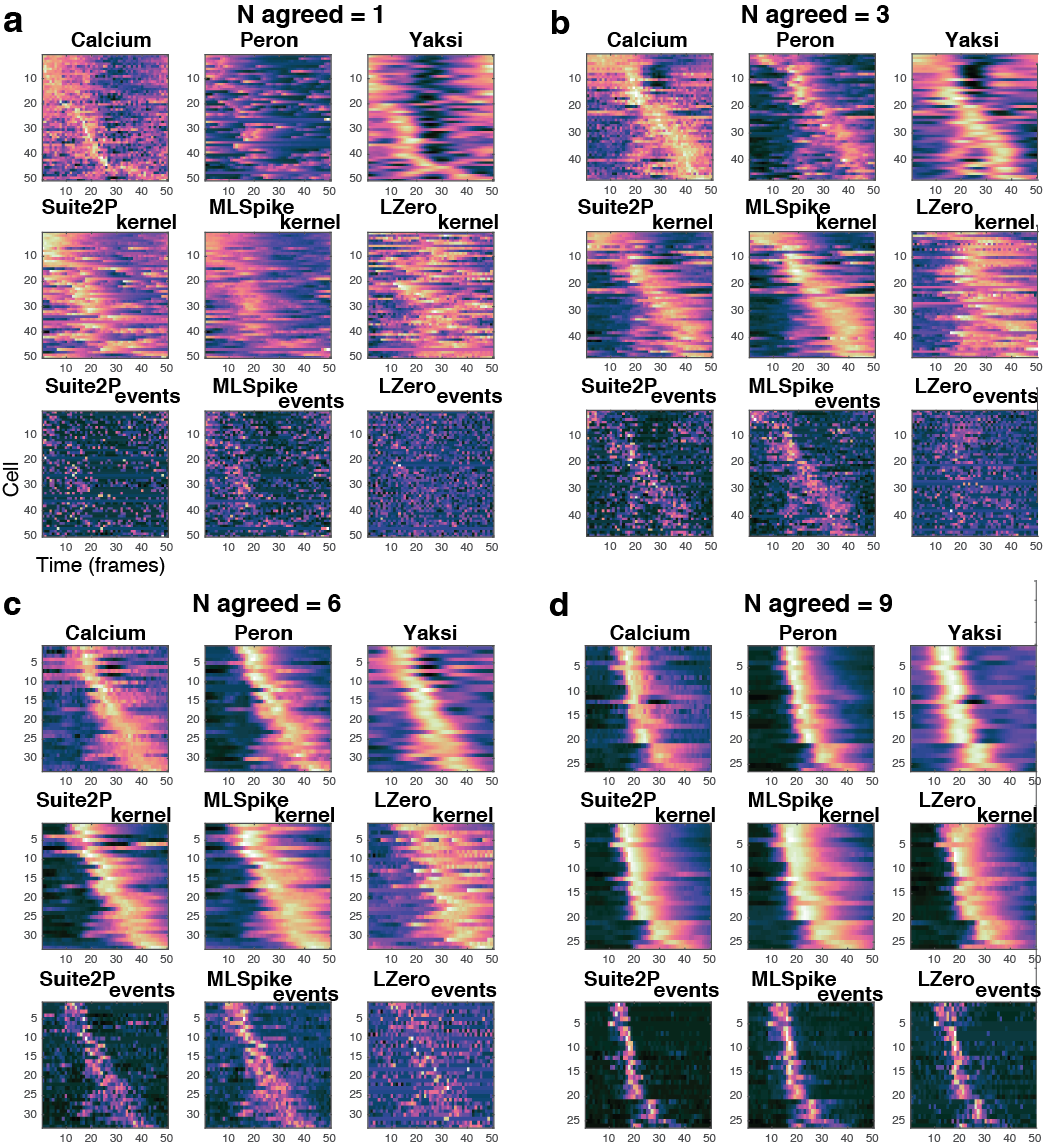
\includegraphics[width=\textwidth]{full_figs/why_deconvolve_F5_2.png}
\caption{\label{fig:tuned_cells_psth}Degree of agreement between methods can identify strongly tuned cells. (a) Example normalised (z-score) trial-average histograms for 50 cells (rows) classified as tuned in an analysis of raw Calcium data. Each subsequent panel shows trial-average histograms for the same cells, but following processing by each of the eight deconvolution/spike inference methods. (b) - (d) as in (a) but showing trial-average data for cells classed as tuned by 3, 6 and all 9 methods. \textbf{TO DO: Add marker to show which methods classify which cells as tuned?}}
\end{figure}


\subsection{Deconvolution and spike inference may degrade the ability to recover precisely timed responses}
%\noindent \emph{\textbf{Results in brief}\\
%- Experimental manipulations or task events may result in precisely timed (+ brief, small amplitude) responses in L2/3 of cortex\\
%- Deconvolution/spike inference is often employed to increase the ability to detect such responses/cells, by reducing background noise and removing the slow kinetics of Calcium changes.\\
%- For clearly tuned cells, this approach appears valid (example PSTH shows temporally sharp peak)\\
%- However, as for task tuning, different methods disagree on the number of tuned cells.\\
%}


Experimental manipulations or task events often result in precisely timed responses in some neurons. To determine whether deconvolution and spike inference improve the temporal precision of analyses such as tuning curves we computed the touch-triggered average for all cells in the example dataset. In the somatosensory system, touch onset is a salient sensory signal known to drive a subset of neurons to spike with short latency and low jitter \citep{OConnor2010-hd, Hires2015-by}. To determine touch tuning for each cell we found the peak in the touch triggered average, and compared the data distribution (one data point per touch) at this time point to a shuffled data distribution (Benjamini Hochberg corrected Mann-Whitney U test). 

Spike inference or deconvolution is often employed to increase the ability to detect temporally sharp responses by reducing background noise and removing the slow kinetics of Ca\textsuperscript{2+} changes. For clearly tuned cells this approach appears valid - in Fig \ref{fig:touch_triggered} (a) the touch-triggered averages for an example cell show a temporally sharp peak around touch for the spike inference methods. However, as for task tuning, different methods disagree on the number of touch-tuned cells. Fig \ref{fig:touch_triggered} (b) shows the proportion of cells classed as touch-tuned after processing signals with each method. Of particular note, the spike inference methods disagree substantially on this score, with one method (MLSpike) estimating 300\% more touch-tuned cells than another (LZero). Without more analysis it is unclear which - if any - is correct.


\textbf{TO DO? Comparison of estimates when deconvolving/inferring spikes vs not\\
\indent - signal to noise \\
\indent - temporal resolution (rise/decay time)}\\



\begin{figure}
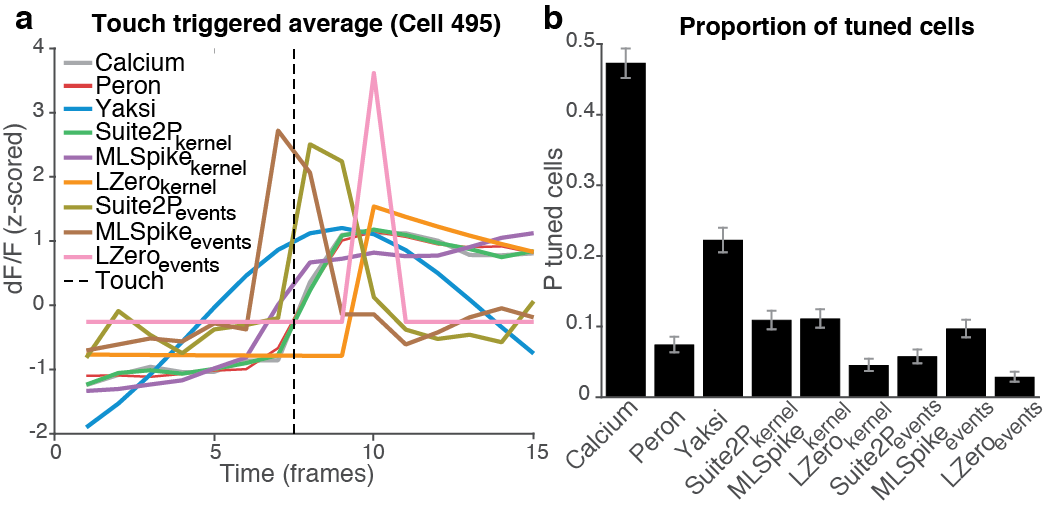
\includegraphics[width=\textwidth]{full_figs/why_deconvolve_F6_3.png} 
\caption{\label{fig:touch_triggered} Touch-related responses. (a) Comparing touch-triggered average (mean deconvolved FR per imaging frame) from different deconvolution methods for one example cell. Touch occurs during frame 7 (dotted line). (b) Number of touch tuned cells varies across methods. A cell is classed as touch tuned if peak touch-triggered activity is significantly greater than shuffled data (Mann-Whitney U test, Benjamini Hochberg corrected). Error bars are Jeffreys intervals}
\end{figure}




%\subsubsection*{Correlations}
% IDEA: Compute PCCs with decorrelated events computed with different parameters. How does the distribution move?

%[trim={50 10 50 10 },clip,width=0.8\textwidth]{pairwise_scatter2.eps}}
%[trim={50 10 50 10 },clip,width=0.8\textwidth]{pairwise_kernel2.eps}}

%\begin{figure}[h!]
%\centering
%\subfigure[]{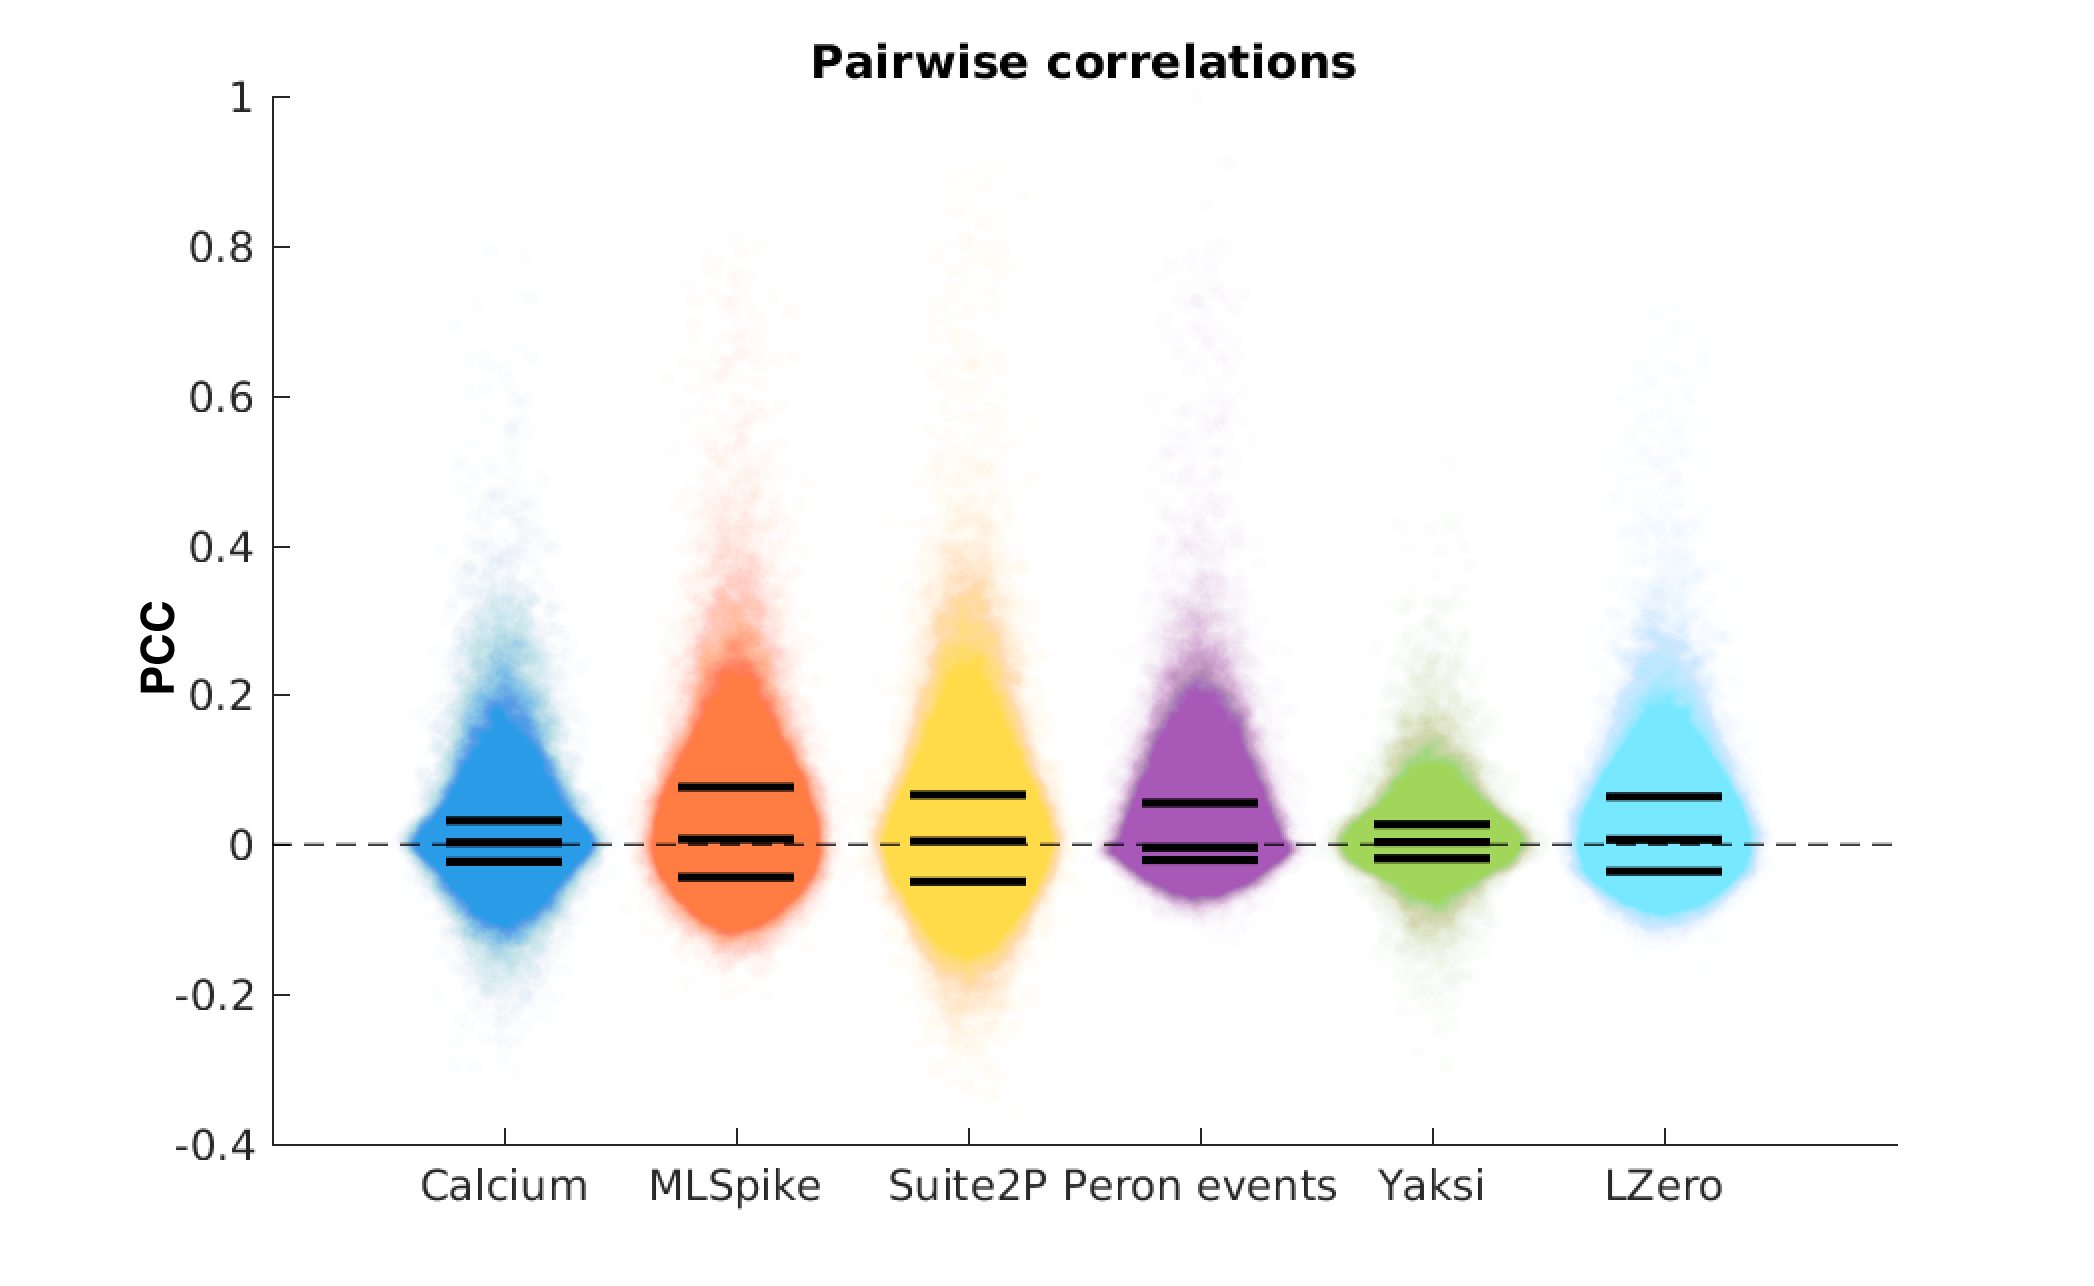
\includegraphics[trim={10 10 10 10 },clip,width=0.45\textwidth]{figs/pairwise_scatter3_alph_pt01.png}}%
%\subfigure[]{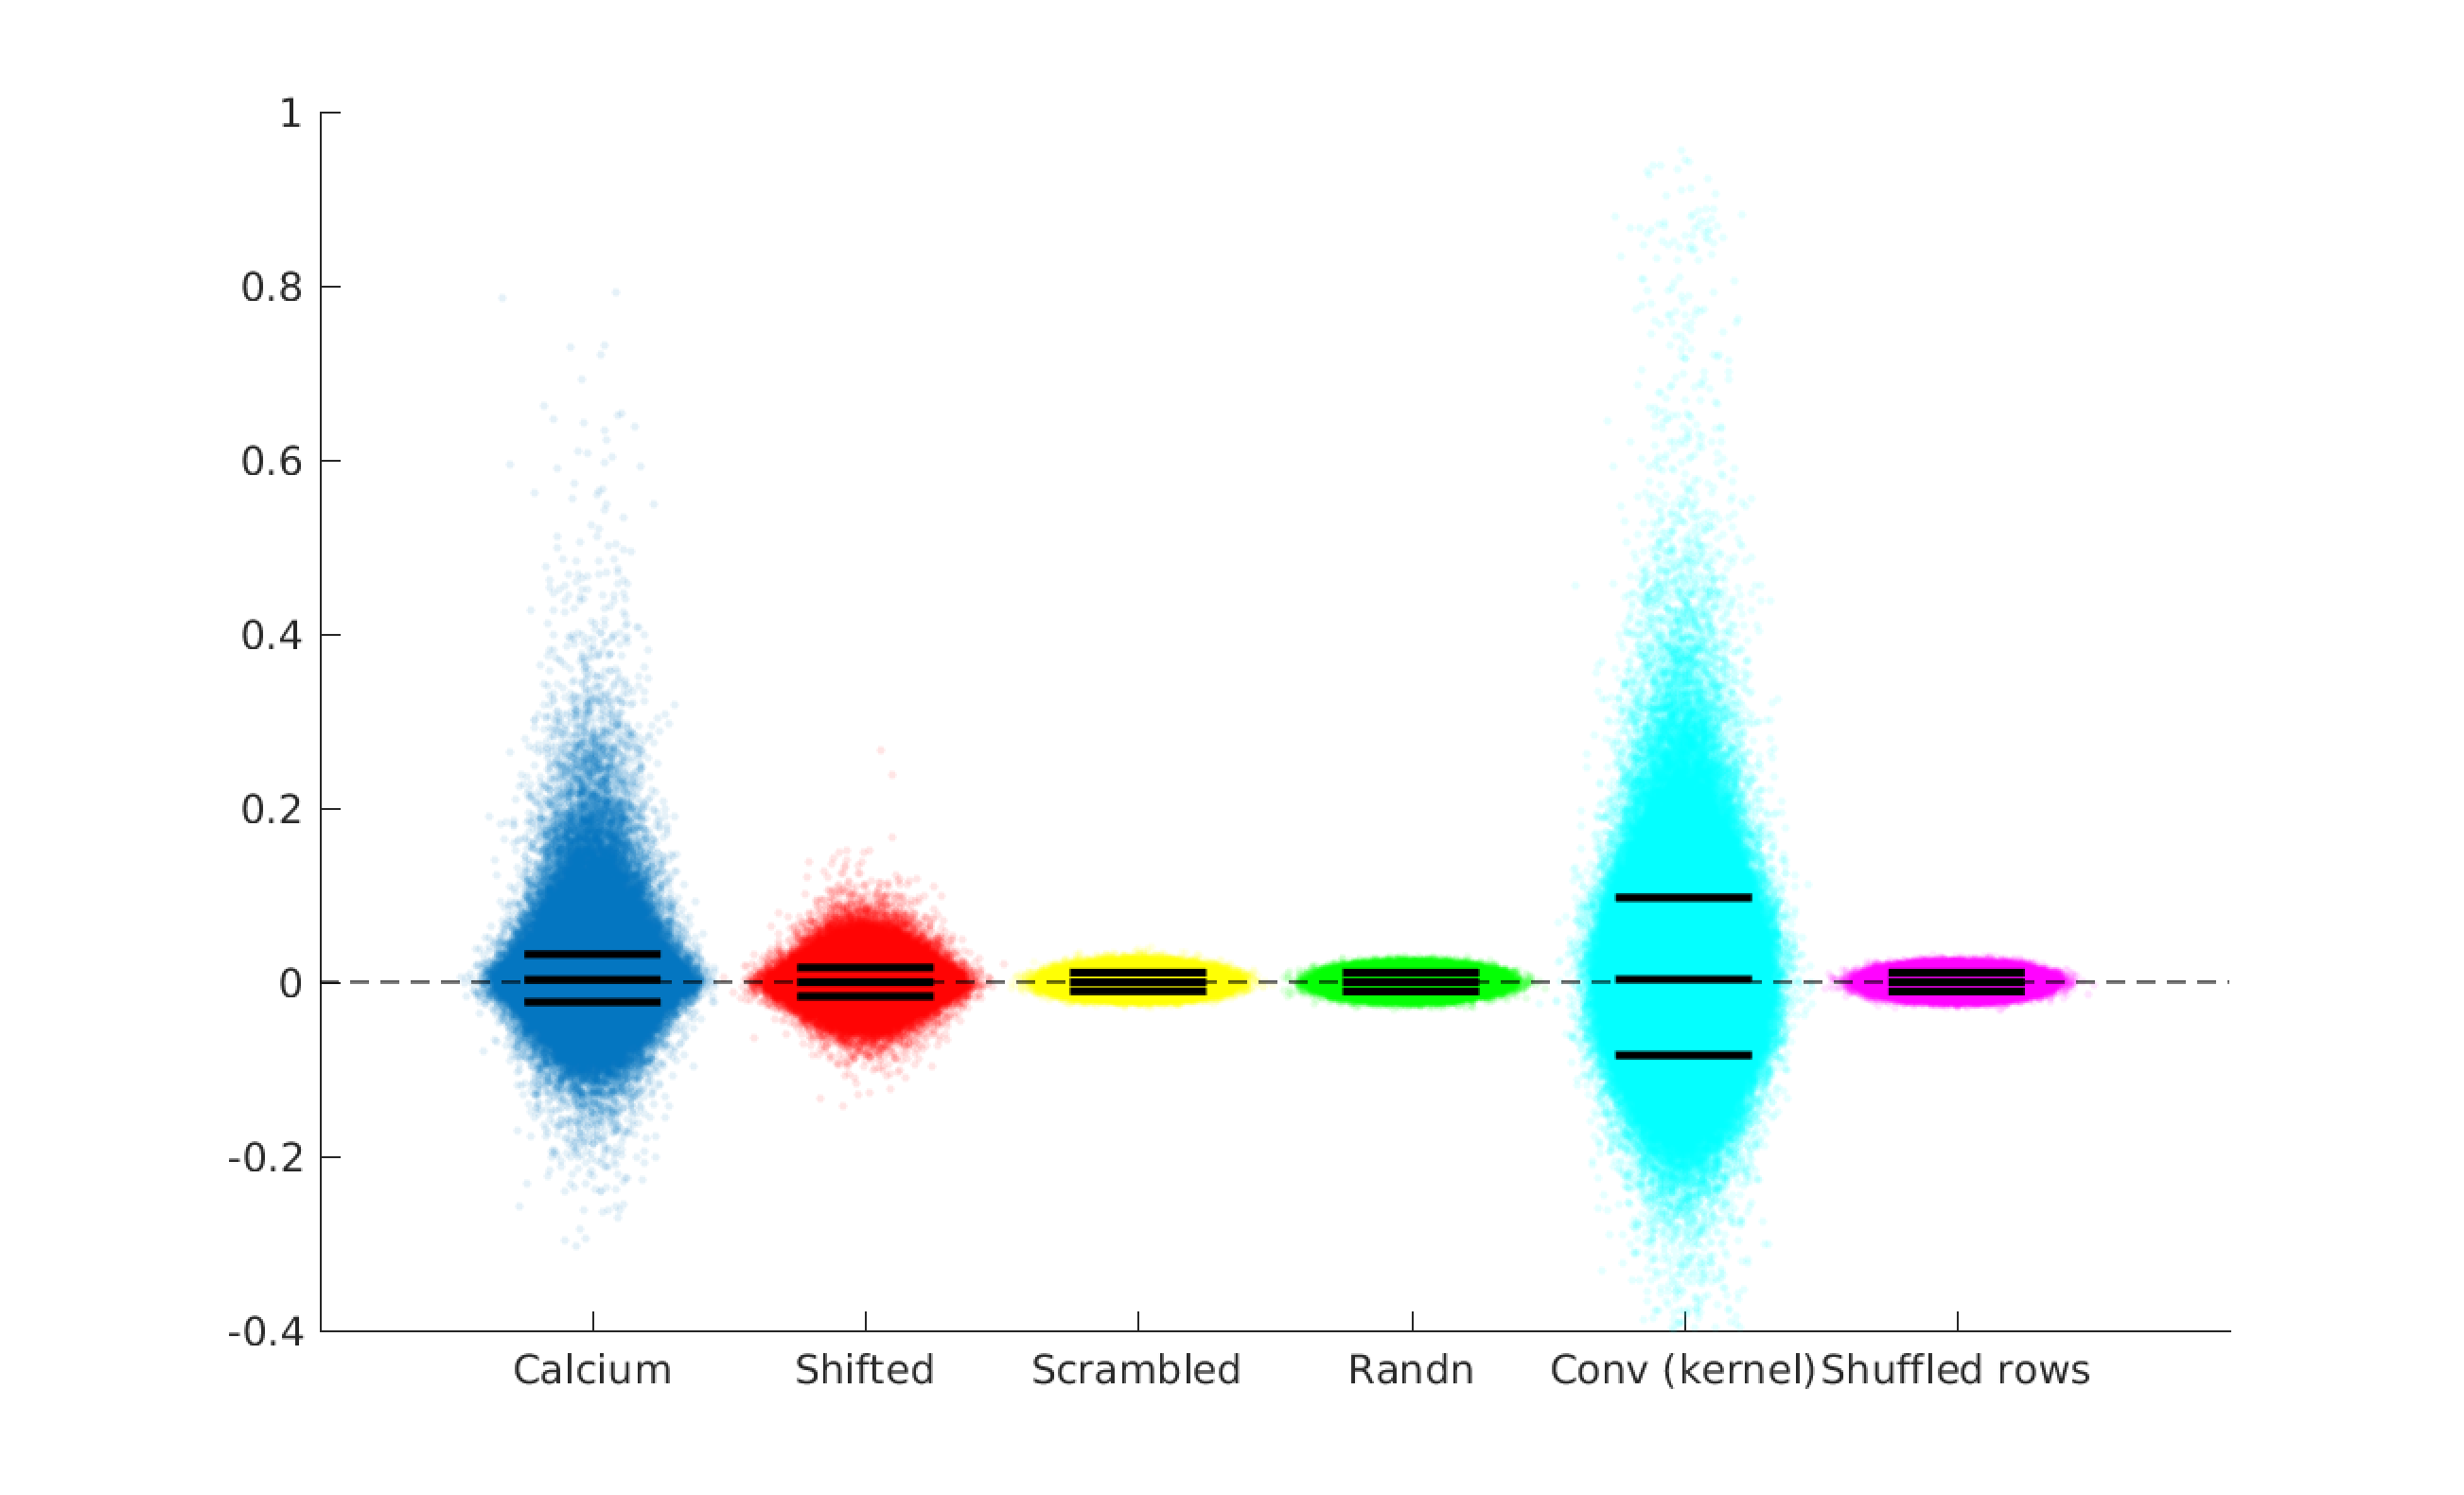
\includegraphics[trim={10 10 10 10 },clip,width=0.45\textwidth]{figs/noise_comparison3CI.png}}
%\subfigure[]{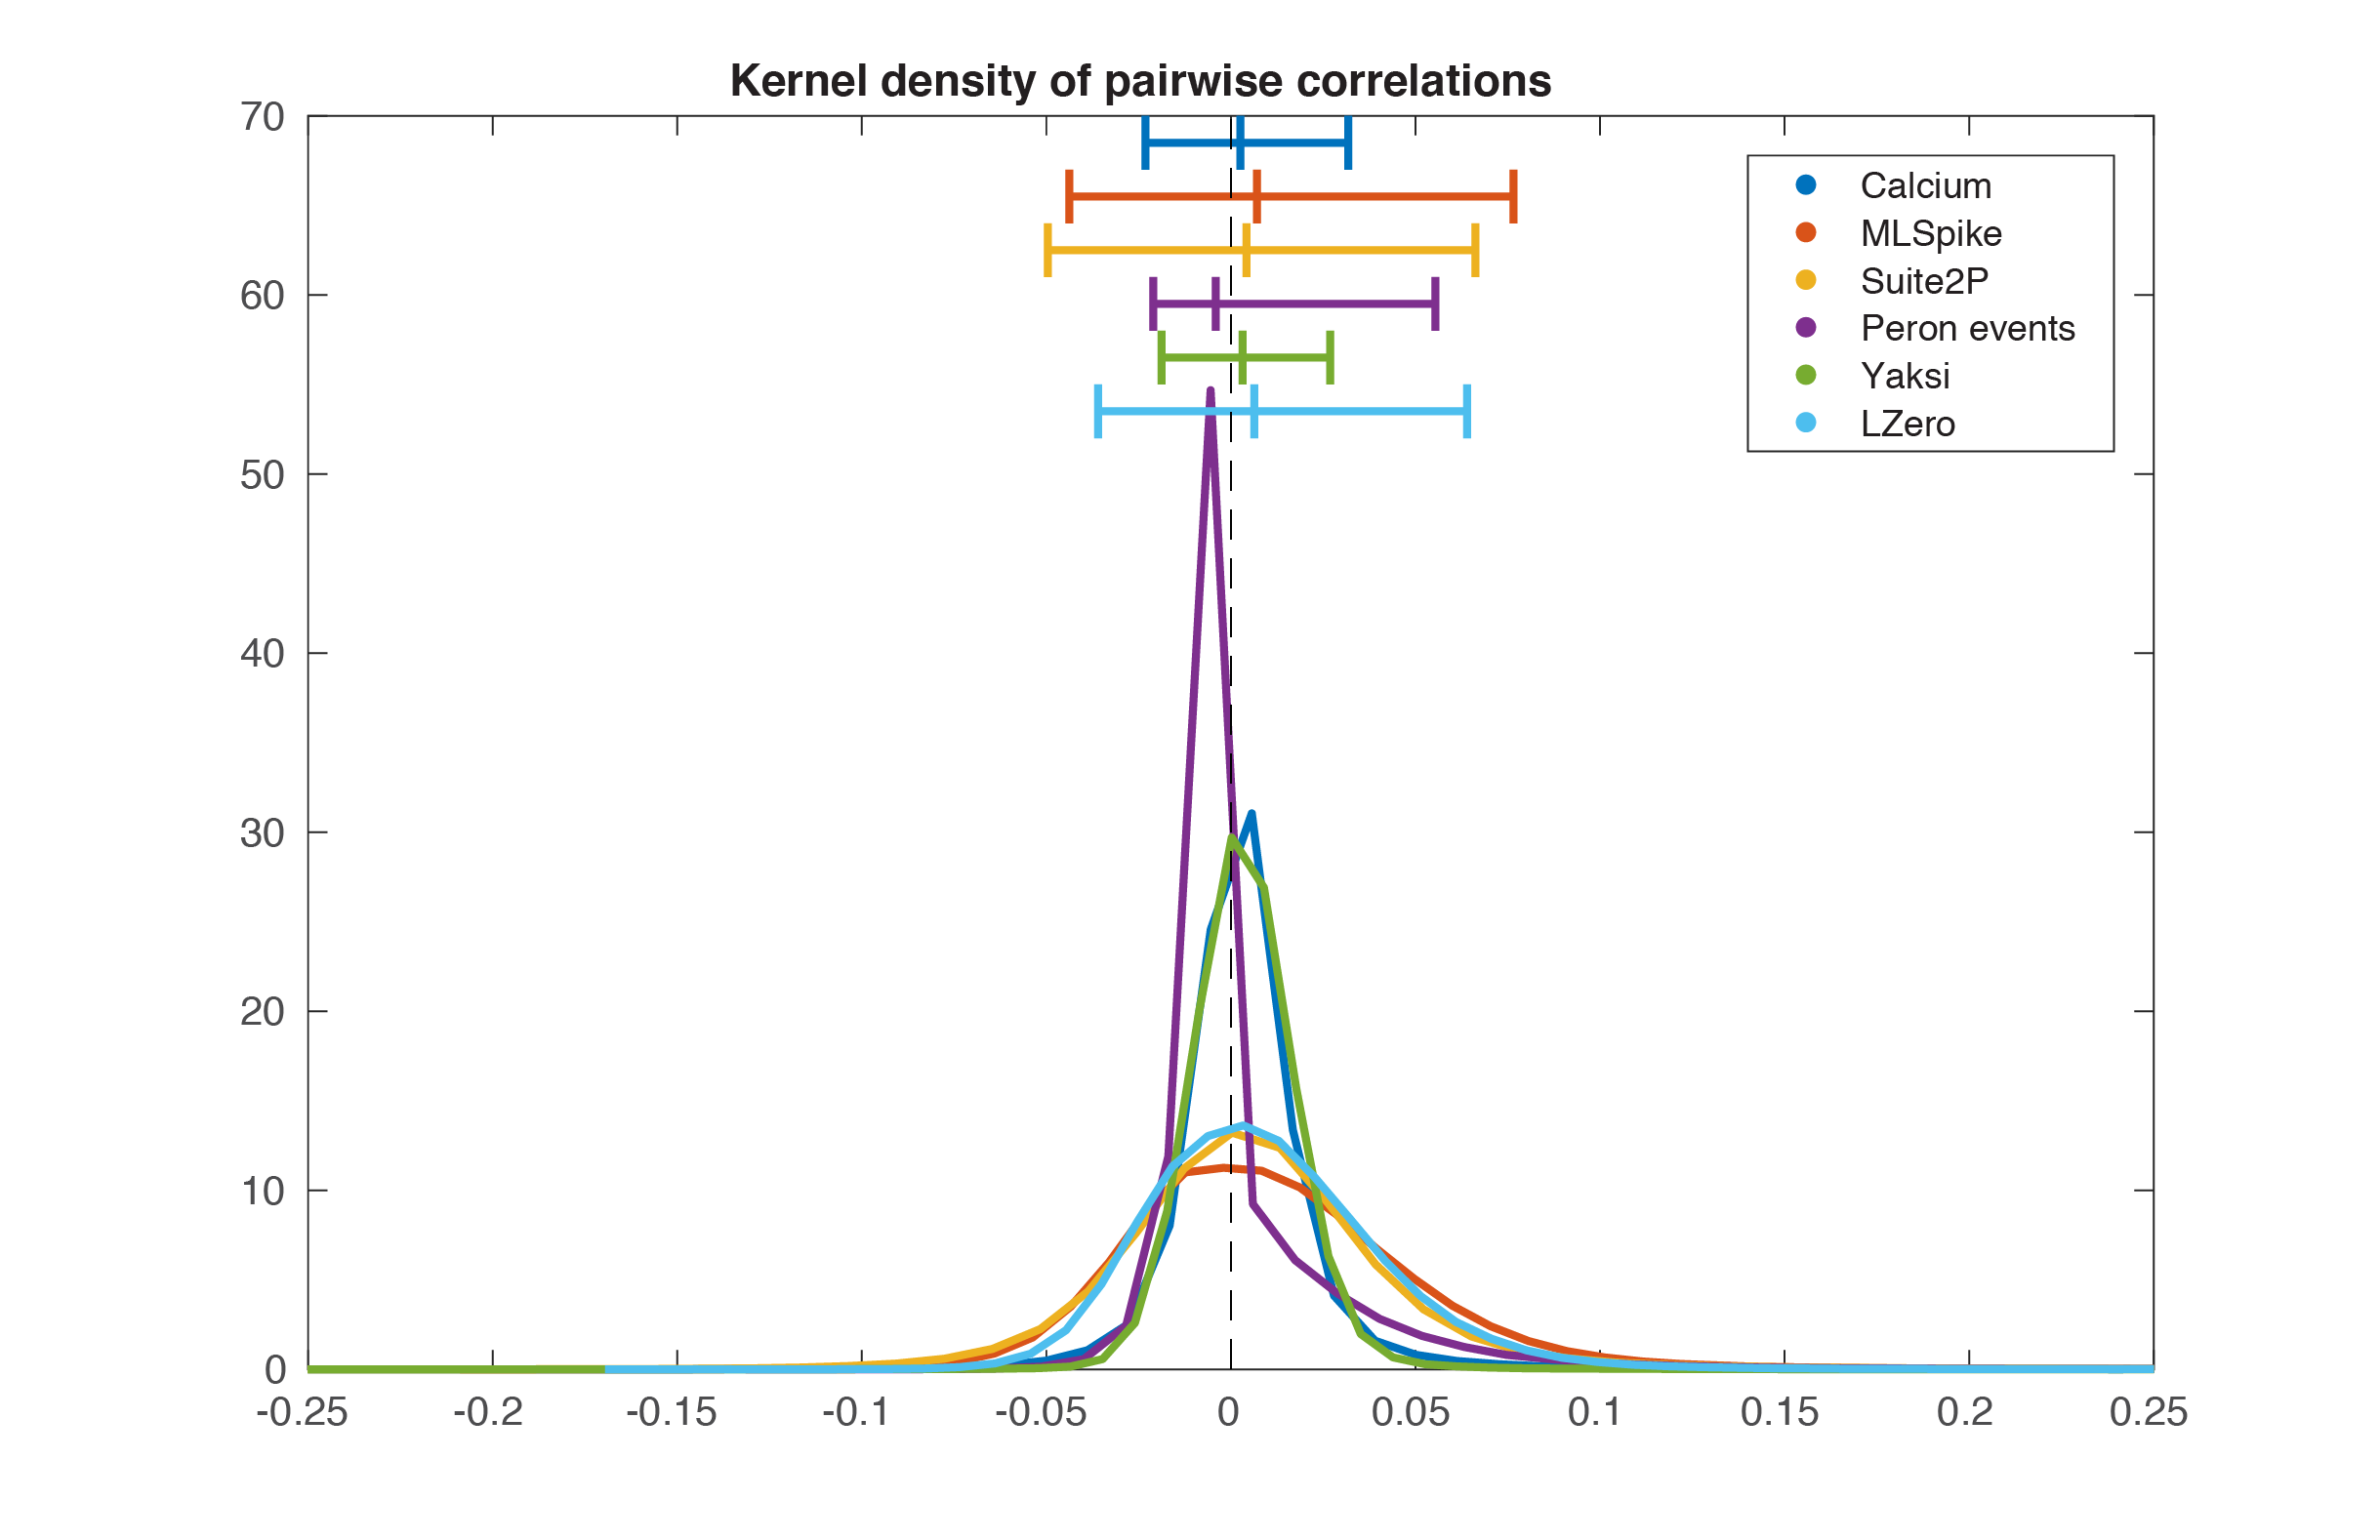
\includegraphics[trim={10 10 10 10 },clip,width=0.45\textwidth]{figs/pairwise_kernel3CI.png}}%
%\subfigure[]{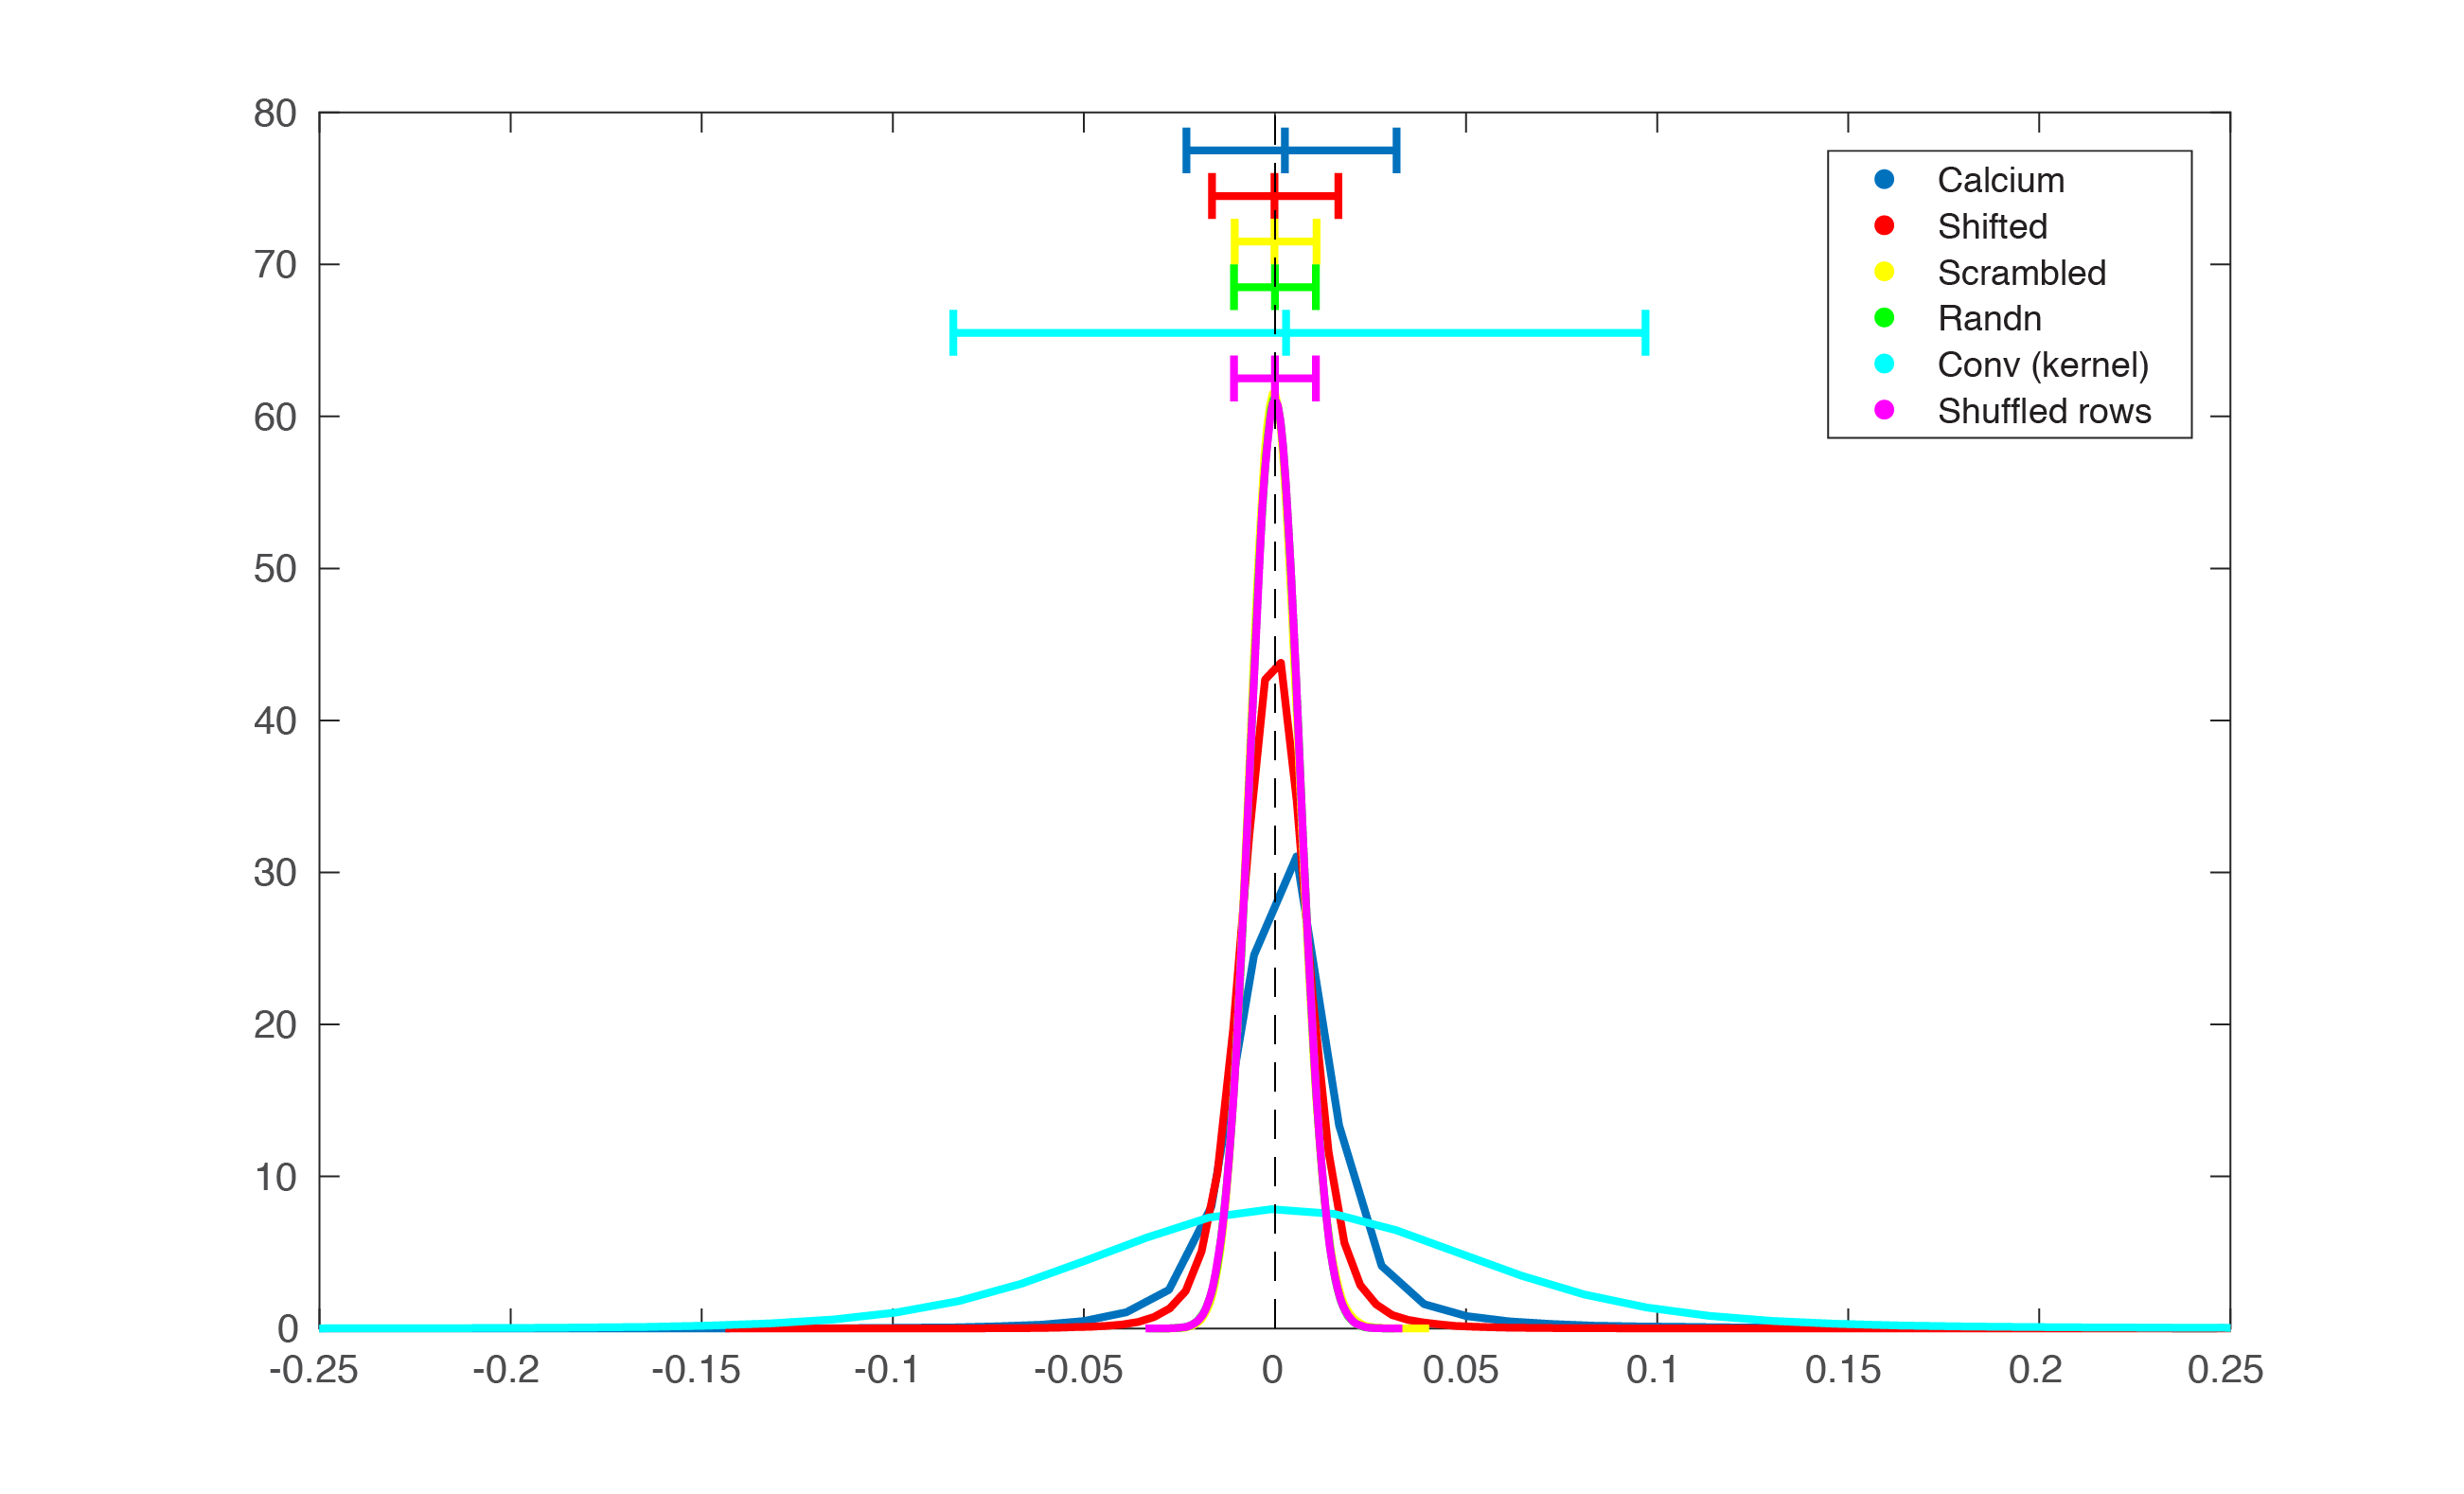
\includegraphics[trim={10 10 10 10 },clip,width=0.45\textwidth]{figs/noise_comparison3_kernel.png}}
%
%\caption{\label{fig:PCCs} Pairwise correlations. (a) For each method (colours) each dot is the Pearson correlation coefficient between each pair of neurons (1203576 unique pairs, excluding self-correlations). X-axis jitter added for clarity. Black lines correspond to 5th, 50th (median) and 95th percentiles of the data. (c) Kernel density plots of data in (a). Lines above density plots correspond to 5th, 50th (median) and 95th percentiles of the data, coloured to match the distributions. (b) and (d) are the same as (a) and (c) but with different permutations or surrogates of the data. Calcium - data as in (a). See main text for details.}
%\end{figure}


%\begin{figure}[h!]
%\centering
%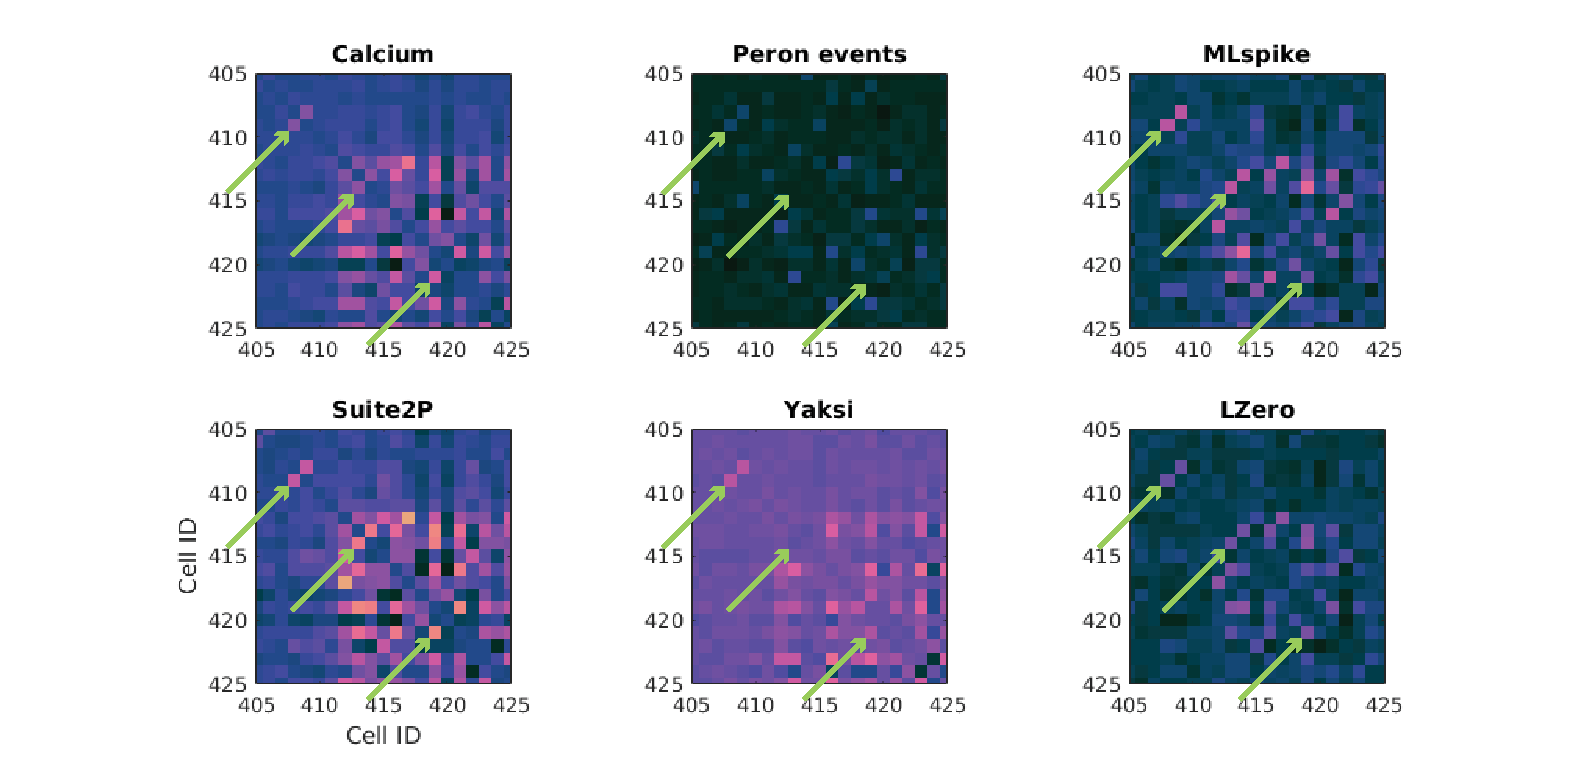
\includegraphics[trim={50 10 50 10},clip,width=0.8\textwidth]{pcc_all_image2_zoom.eps}
%\caption{\label{fig:PCC_example} Peron events and Yaksi may actively decorrelate neurons. Each panel shows a subset of pairwise correlations between neurons from one session of data from Peron et al 2015, one panel for each method. Some pairs (arrows) showing high correlation across methods are missing (middle arrow) for the Peron events and Yaksi methods.}
%\end{figure}

%\subsubsection*{Tuning}

%\clearpage
%\subsection*{Deconvolution does not improve the precision of temporal resolution under realistic conditions}
%\emph{Comparison of estimates when deconvolving vs not\\
%\indent - signal to noise \\
%\indent - temporal resolution (rise/decay time)\\
%\indent - TO DO: Repeat this analysis with deconvolved events\\
%\indent - TO DO: Temporal correlations. Pick small number of cells e.g. of touch tuned vs some other parameter, and compute their correlations over time. Yaksi and Friedrich showed an advantage in their hands.\\}


%\begin{figure}[h]
%\centering
%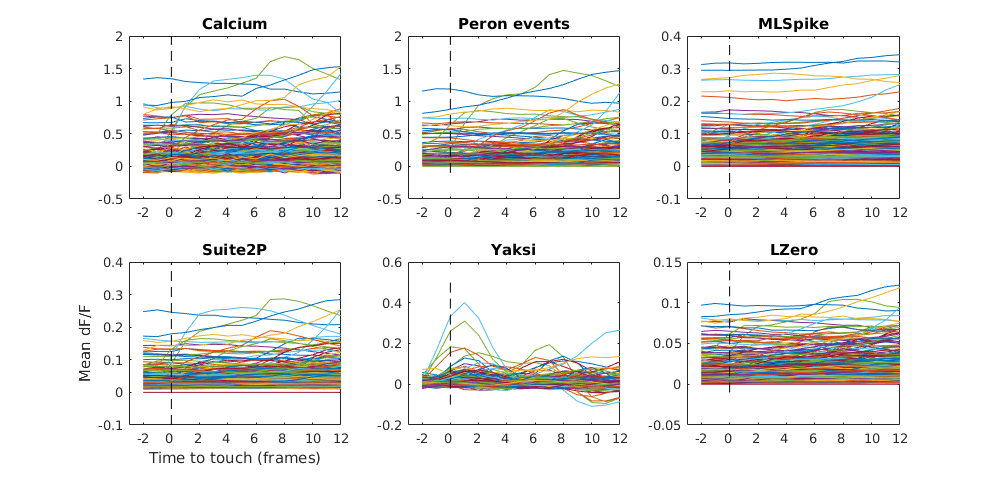
\includegraphics[width=1\textwidth]{tth_all.png}
%\caption{\label{fig:tth_all} Comparing touch-triggered average (mean deconvolved FR per imaging frame) from different deconvolution methods for one all cells. Touch occurs at time zero. Only the Yaksi method shows a temporally sharp touch response.}
%\end{figure}

%\begin{figure}[h]
%\centering
%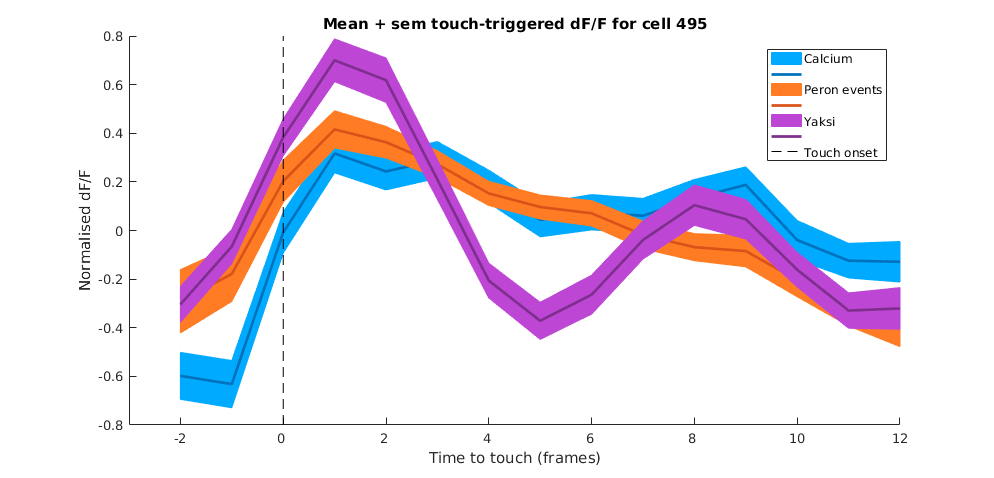
\includegraphics[width=1\textwidth]{tth_495.png}
%\caption{\label{fig:tth_495}Comparing touch-triggered average (mean and s.e.m) from different deconvolution methods for one cell. Touch occurs at time zero. While the Yaksi method shows a temporally precise touch response, decaying within 1s (<7 frames), the Calcium and Peron events show a sustained response.}
%\end{figure}

%\begin{figure}[h]
%\centering
%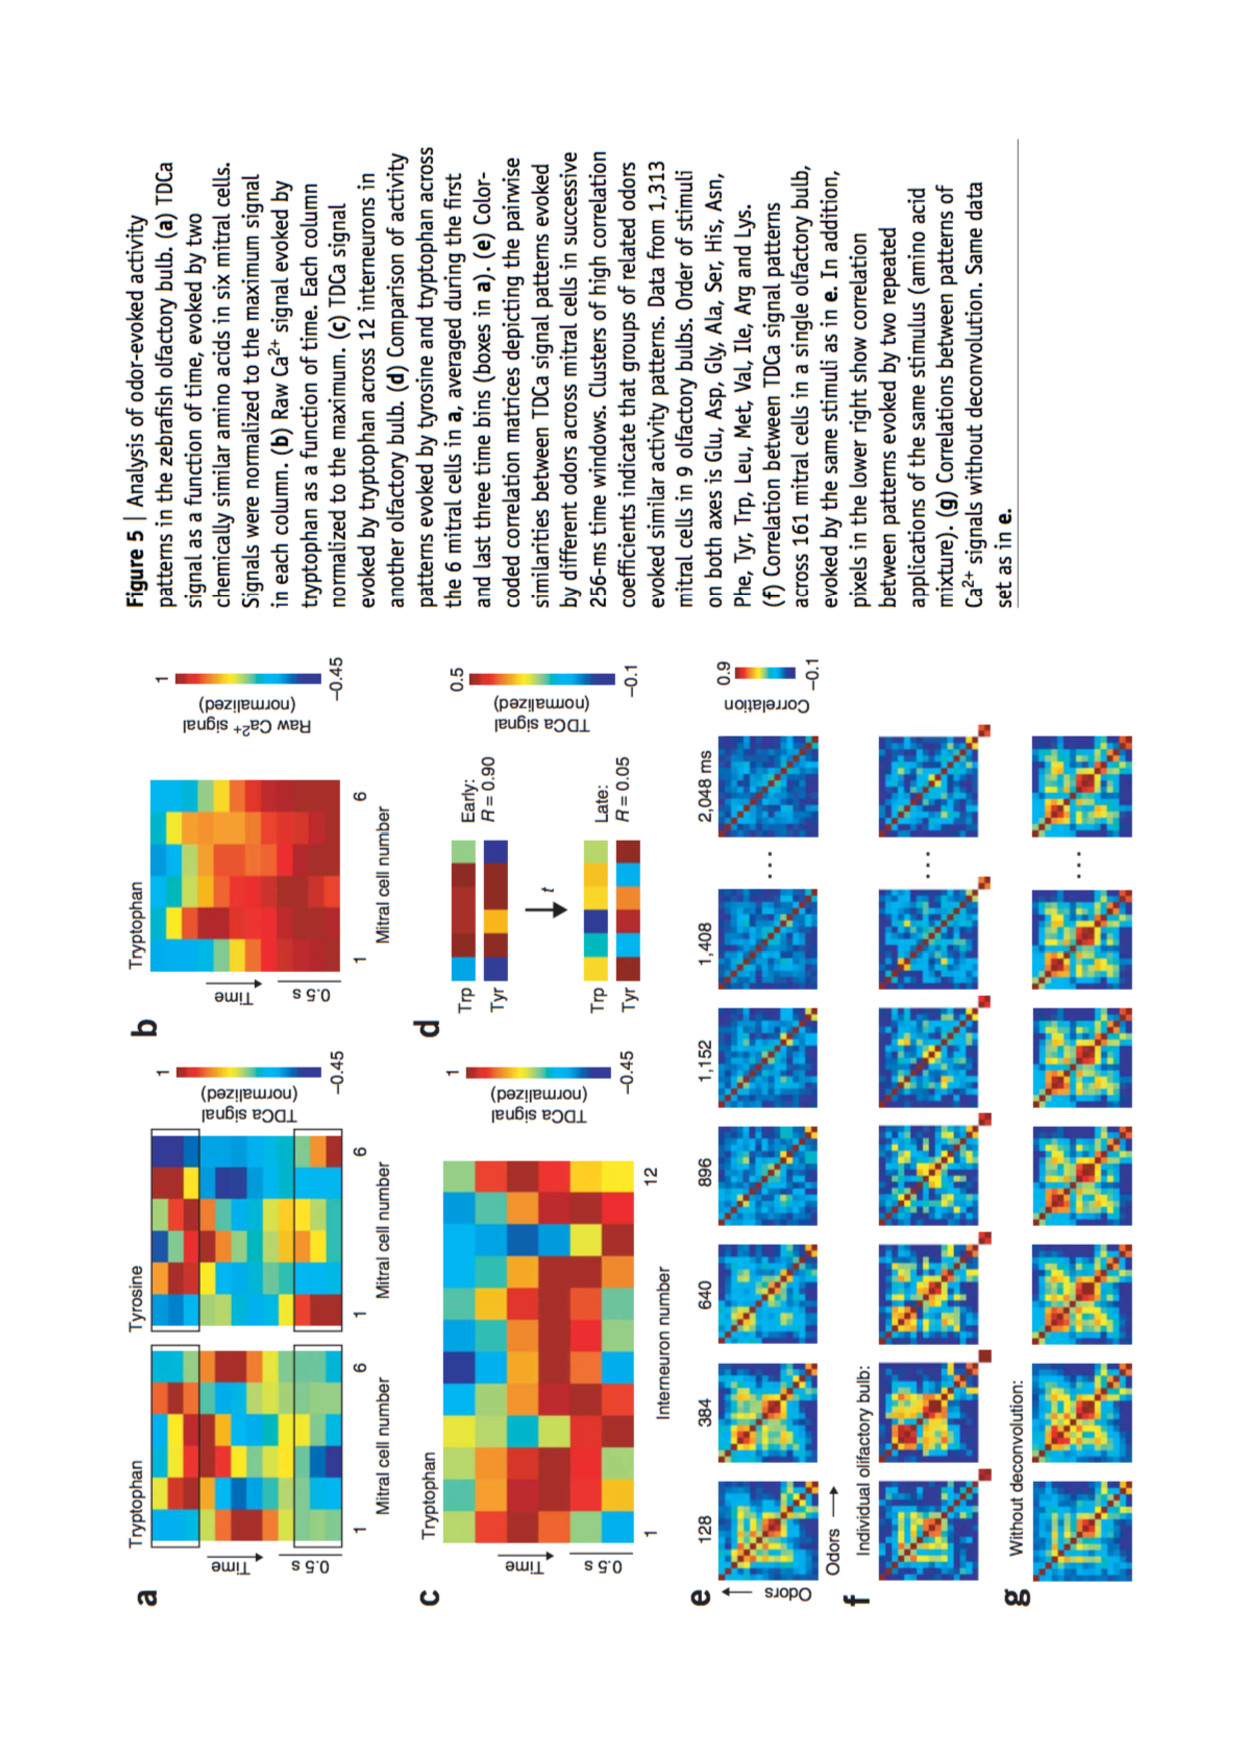
\includegraphics[height=\textwidth, angle = 270]{Yaksi_results2.pdf}
%\caption{\label{fig:Yaksi_time} Deconvolution resolves the fine timescale of pairwise correlations, fig from Yaksi and Friedrich (2006). Perhaps a touch-triggered or 'persistent delay period activity' version of this would be interesting?}
%\end{figure}


\subsection{Pairwise correlation distributions are affected by spike inference and deconvolution}
%\noindent \emph{\textbf{Results in brief}\\
%- Many population analyses involve interpretation of pairwise correlations between cells\\
%- Deconvolution is designed to remove noise, while spike inference will sharpen temporal responses, which will lead to more accurate estimates of pairwise correlation\\
%- In our analysis, different methods result in different estimates of pairwise correlation.\\
%- Correlations are not just scaled - some pairs that appear correlated from processing by one method are uncorrelated when processed with another method\\
%- Some differences in pairwise correlation distributions may be caused by introduction of noise (more symmetric distributions) or smoothing (broader distributions).\\
%- Specifics:\\
%\indent - Some methods agree with each other (Suite2P$_{kernel}$,MLSpike$_{kernel}$), some actively decorrelate (Peron, Spike inference methods)}\\



A goal of many Ca\textsuperscript{2+} imaging experiments is to record from populations of neurons, and then perform clustering or dimensionality reduction. These analyses often rely on estimates of pairwise correlations (CITATION NEEDED). The methods tested in this study are designed to remove noise and sharpen temporal responses, which would lead to more accurate estimates of pairwise correlation. Figure \ref{fig:cxy_dist} (a) and (b) show the distributions of pairwise correlation coefficients computed separately for each method. To aid interpretation of these results we also computed pairwise correlations for five different data surrogates (see methods).



\emph{Description}
Deconvolution/de-noising methods (Yaksi, Suite2P$_{kernel}$, MLSpike$_{kernel}$, LZero$_{kernel}$) have broad distributions more similar to that resulting from smoothing the raw Ca\textsuperscript{2+}. Suite2P$_kernel$ and Peron have median PCCs below zero, suggesting these methods are actively decorrelating the data (choosing parameters that penalise false-positives). Yaksi's distribution is symmetric (like all the noise surrogates) suggesting dirt has been added to the data. LZero$_{kernel}$ resulted in very sparse time series, so the long tail of positive values are likely to be the large group of almost silent cells. Spike inference methods all have sharp peaks just below zero. Not sure why.\\

\emph{Interpretation (SPECULATIVE - DISCUSS WITH MARK):}\\ 
\indent - Deconvolution/spike inference is always a trade-off between false positives and misses - meaning you get both - resulting in altered pairwise correlations, and their distributions\\
- Deconvolution/ de-noising, by eliminating photonics shot noise (smoothing the time series), increases the temporal correlations in the data, leading to stronger correlations\\
- Choosing analysis parameters that result in firing rate distributions peaked close to zero (reducing false positives) inevitably lead to more miss errors, and therefore actively decorrelate.\\
\indent - Spike inference is never going to be perfect. Miss real spikes + overestimate background rates (spike inference is additive, so adding background spikes is inevitable. See also \citealt{Ganmor2016-uf} on this point), therefore correlation estimates are noisier (due to false positives/misses ) and biased (due to misses therefore decorrelation, or false positives therefore higher mean correlations)\\
%\indent - TO DO (?) repeat this analysis but with deconvolved events where available




%\begin{figure*}
%\floatbox[{\capbeside\thisfloatsetup{capbesideposition={right,top},capbesidewidth=0.3\textwidth}}]{figure}[\FBwidth]
%{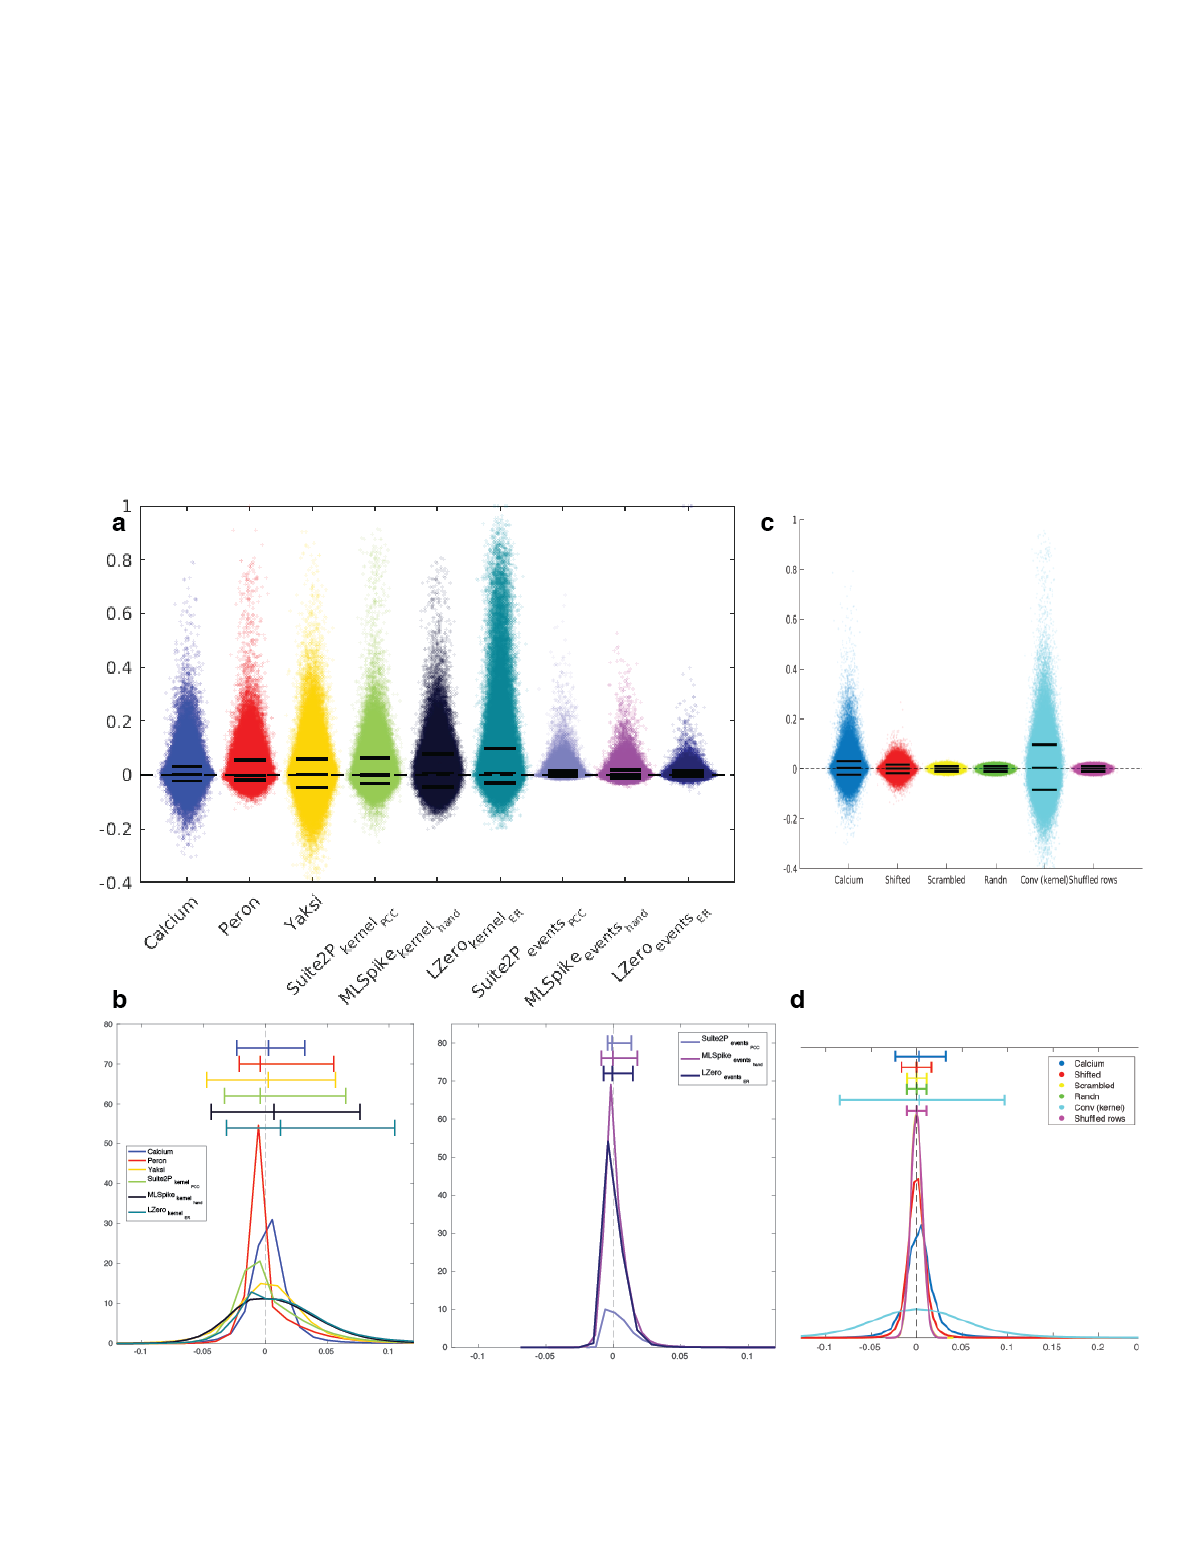
\includegraphics[trim={10,30,10,100},clip,width=0.7\textwidth]{full_figs/why_deconvolve_F9.png}}
%{\caption{\label{fig:cxy_dist}}}
%\end{figure*}

%\newpage


Looking in more detail at a subset of 50 cells, Fig \ref{fig:cxy_comparison} (a) shows that the disagreement between methods can be seen at the level of individual pairs of neurons.  Correlations are not just scaled - some pairs that appear correlated following processing by one method (yellow box and arrows) are uncorrelated when processed with another method. Other pairs are consistently correlated across methods (green box and arrows). 

\begin{figure*}
\floatbox[{\capbeside\thisfloatsetup{capbesideposition={right,top},capbesidewidth=0.3\textwidth}}]{figure}[\FBwidth]
{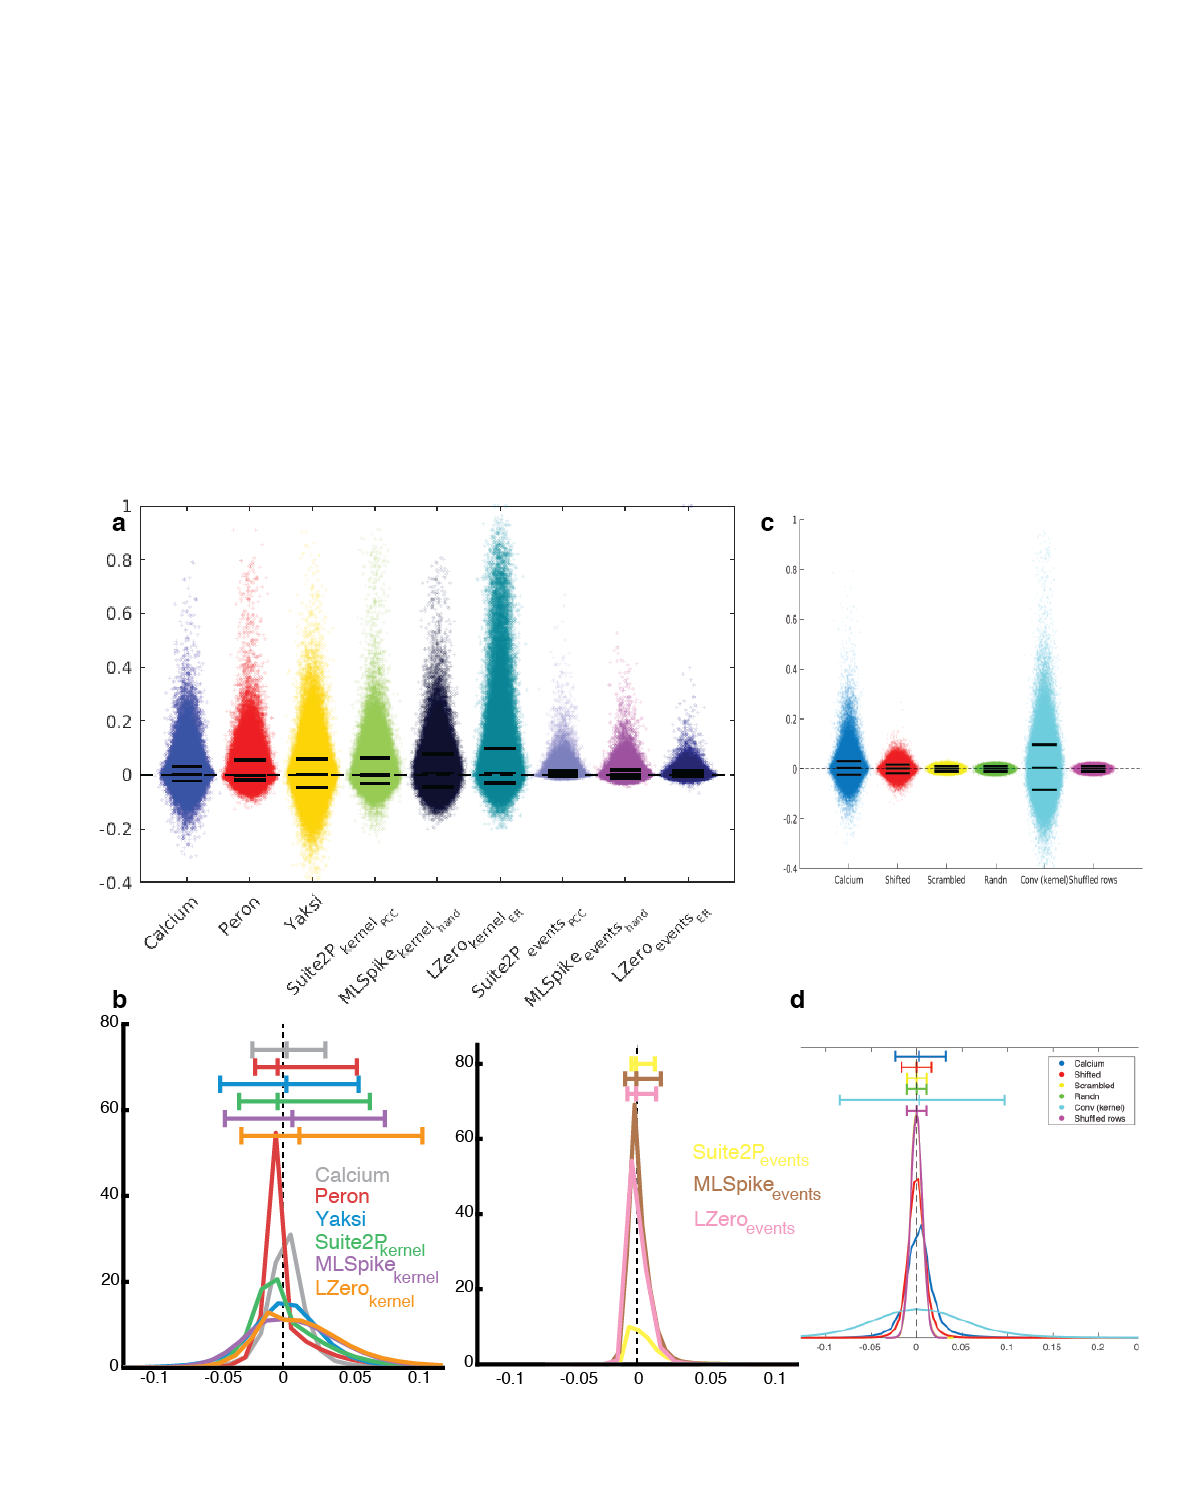
\includegraphics[trim={23 23 10 120}, clip, width=0.7\textwidth]{full_figs/why_deconvolve_F9_2.png}}
{\caption{\label{fig:cxy_dist}Pairwise correlation distributions. (a) Pairwise correlations between all cells (y-axis) following processing with all deconvolution/spike inference methods (x-axis jitter added for clarity). Solid black lines are 5th, 50th and 95th percentiles. (b) Pairwise correlation kernel density functions for all methods.  Vertical lines are medians and 5th, 50th and 95th percentiles. (c) and (d) as in (a) and (b) for different randomised versions of the data, to aid interpretation of distribution changes in (a) and (b).}}
\end{figure*}

Fig \ref{fig:cxy_comparison} (b) shows the correlation between correlation matrices for different methods, showing how similar the correlation matrices are across methods. In Fig \ref{fig:cxy_comparison} (c) the same data is shown but separating the spike inference methods (right) from the others for better comparison. Though there are some exceptions (Fig \ref{fig:cxy_comparison} (a)), overall there is broad agreement within method classes on which cells are more or less correlated. In particular, Suite2P$_{kernel}$ and MLSpike$_{kernel}$ are correlated with one another, as are Suite2P$_{events}$ and MLSpike$_{events}$. LZero appears to form unique correlation matrices, correlating only with itself (LZero$_{kernel}$ and LZero$_{events}$ correlate only with one another). Yaksi correlates highly with the raw Ca\textsuperscript{2+}, reflecting the fact that Yaksi changes the time series the least of the pre-processing methods. 




\begin{figure*}
\floatbox[{\capbeside\thisfloatsetup{capbesideposition={right,top},capbesidewidth=0.3\textwidth}}]{figure}[\FBwidth]
{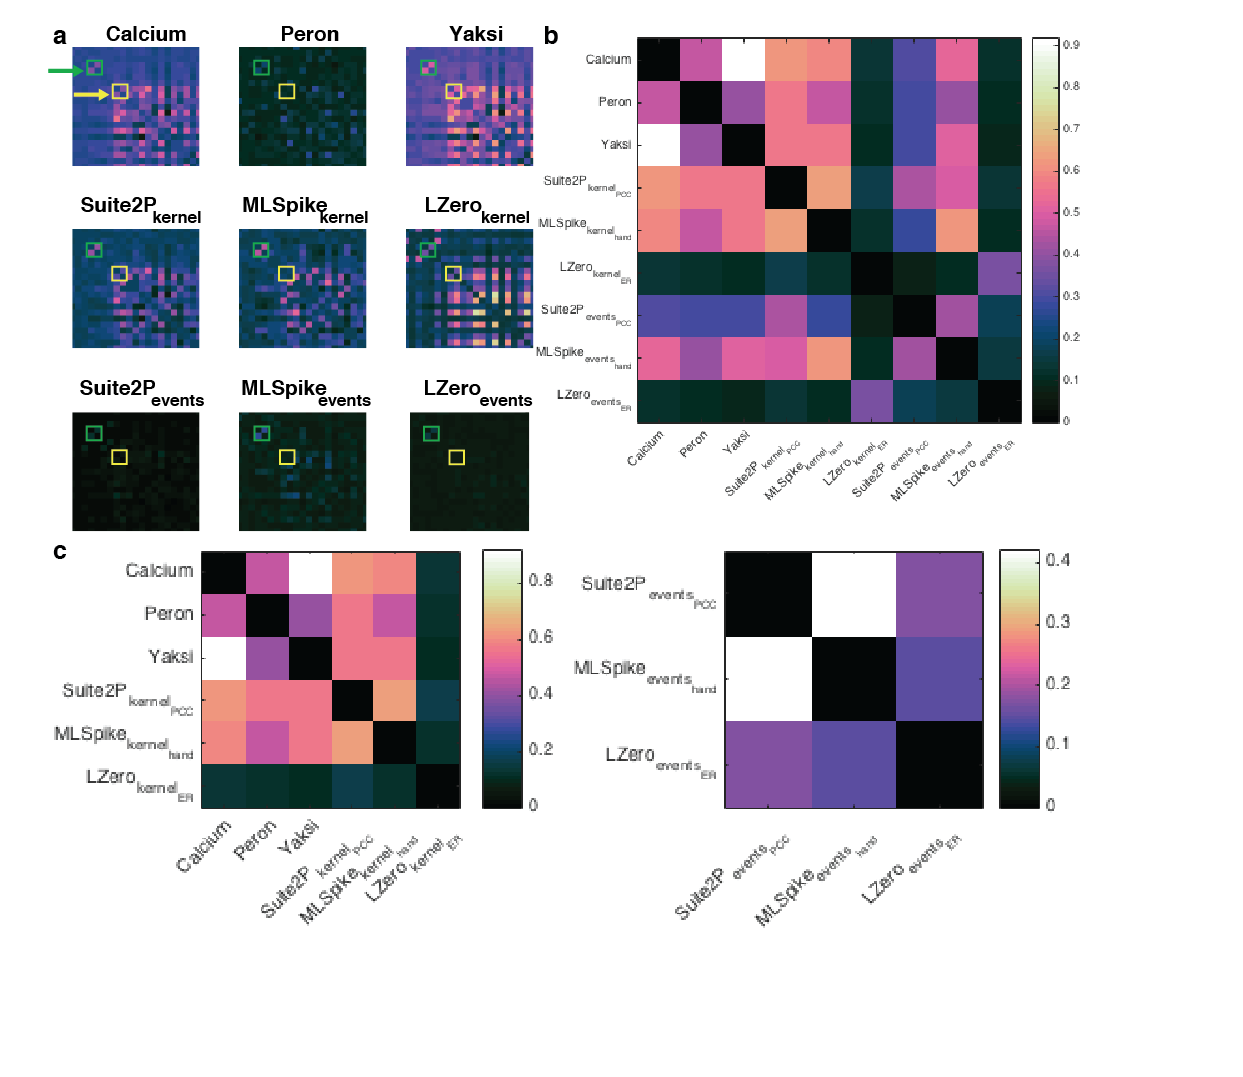
\includegraphics[trim={10 35 35 5}, clip, width=0.7\textwidth]{full_figs/why_deconvolve_F8.png}}
{\caption{\label{fig:cxy_comparison}Pairwise correlations. (a) Example pairwise correlations for 50 cells. Some pairs of cells are consistently correlated across different methods (green arrow and boxes). Other pairs appear correlated when processed with one method but not with others (yellow arrow and boxes). (b) Correlation between pairwise correlation matrices for each method. Some methods result in similar correlation matrices (e.g. Yaksi and Calcium), while others generate distinct correlation matrices (LZero methods). (c) as in (b) but split to show continuous methods (left) or spike inference methods (right). \textbf{add label to c saying 'spike inference' and 'continuous/de-noising'}}}
\end{figure*}


\subsection{Deconvolution and spike inference results in different estimates of the dimensionality of population recordings}
%\emph{Logically, this needs to go after the correlation distribution results: PCA etc are operations *on* the correlations between neurons, so from the different distributions of correlations we can already anticipate differences in dimensionality. 
%But, as it turns out, the fact that the three spike-inference methods have broadly  the same overall distribution of correlations does not predict the similarity of their dimensionality}

%\noindent \emph{\textbf{Results in brief}\\
%- Dimensionality reduction techniques such as PCA allow researchers to make sense of large scale neuroscience data\\
%- Often performed as a pre-processing stage ahead of visualisation or clustering, PCA provides an estimate of the dimensionality of data - the number of orthogonally separable sources of variance in the data\\
%- Dimensionality estimates are affected by deconvolution/spike inference choices\\ 
%- Depending on the approach, the same dataset can appear low or high dimensional\\
%- TO DO: add back in (in supplement) results when deconvolutino/spike inference parameters are different?\\
%}

Dimensionality reduction techniques such as eigendecomposition allow researchers to make sense of large scale neuroscience data. Often performed as a pre-processing stage ahead of visualisation or clustering, eigendecomposition provides an estimate of the dimensionality of data - the number of orthogonally separable sources of variance in the data. We applied eigendecomposition to the example data from \citealt{Peron2015-kd} processed by the eight different de-noising, deconvolution and spike-inference methods. Fig \ref{fig:dimensionality} shows the cumulative variance explained with increasing eigenvectors (dimensions) for each method. The number of dimensions required to explain 80$\%$ of the data varies dramatically across methods from 120 (Peron) to 720 (Calcium) \textbf{N.B. eyeballed estimates - get real numbers!}. This result indicates that the same dataset can appear low dimensional ($<$10$\%$ dimensions required to explain 80$\%$ of the variance) to high-dimensional ($\sim$50$\%$ of dimensions required).

\textbf{TO DO: add back in (in supplement) results when deconvolution//spike inference parameters are different? In the first attempt at this analysis there was another group of methods closer to the Pachitariu result of 'full dimensionality'}


\begin{figure}
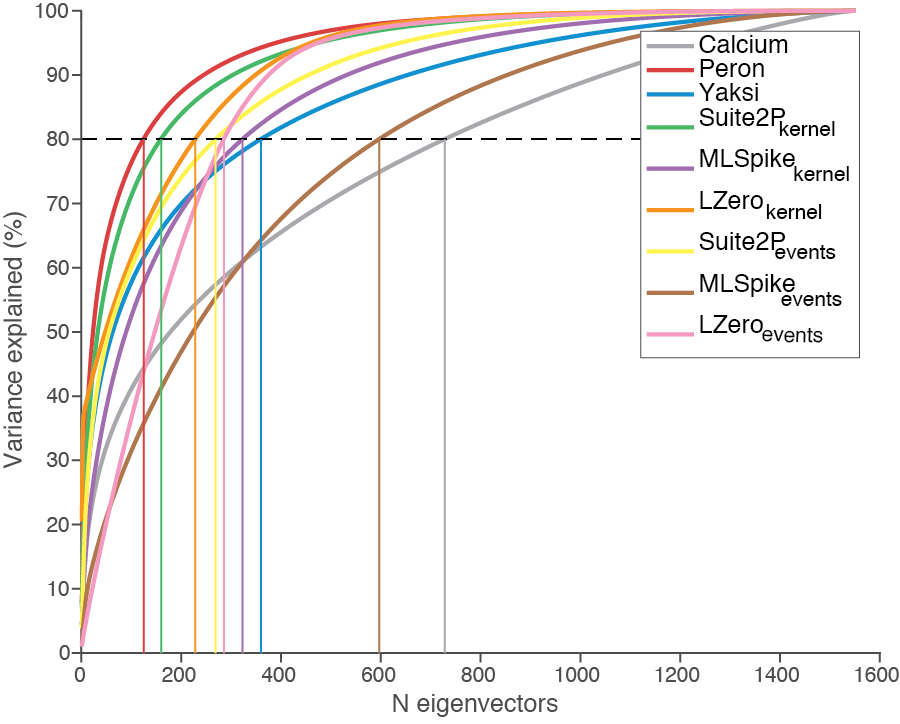
\includegraphics[width=0.9\textwidth]{full_figs/why_deconvolve_F7_2.png}
\caption{\label{fig:dimensionality}Cumulative variance explained by N eigenvectors following Principal Components Analysis. Different spike inference/deconvolution methods result in different estimates of the dimensionality of the data. For example, 80$\%$ of the variance can be explained by 120 or 720 eigenvectors (orthogonal dimensions) depending on the processing method used. \emph{FIX COLOURS: Can't tell which one is the calcium, which the $MLzero_{kernel}$, and which the $LZero_{events}$. Use grey for the raw Ca2+. MDH: To give some idea of how this tunes between “low” and “high” dimensions, replot these “N” as a strip-plot (1D scatter) of the percentage of the population. The N=720 means we can’t describe the data in much less than half the available dimensions = very high dimensional. Whereas the 120 = 10$\%$ of the available dimensions = low dimensional.}}
\end{figure}




%\clearpage
\subsection*{Spike inference does not automatically remove experimental artefacts}
\textbf{MDH: Not sure we're going to include this - perhaps first need to see the proper version of the figure with the dip clearly visible in the deconvolved and inferred spike time-series}
Apart from improving estimates of neural activity, spike inference is also used to remove artefacts from the data such as slow drifts in fluorescence across experiments, or differences in single-spike fluorescence across cells. In head fixed imaging experiments, licking behaviours can lead to a dip in Ca\textsuperscript{2+} fluorescence (Simon Peron, personal communication. Pachitariu COSYNE poster on correcting drift {\href{https://figshare.com/articles/Drift_correction_for_electrophysiology_and_two-photon_calcium_imaging/5946574}{{\color{blue} FIGSHARE LINK TO POSTER}}}). However, Figure \ref{fig:lick_PSTH} shows that this dip is also present in deconvolved traces (TO DO ADD BETTER FIG).

\begin{figure}[H]
%\subfigure[]{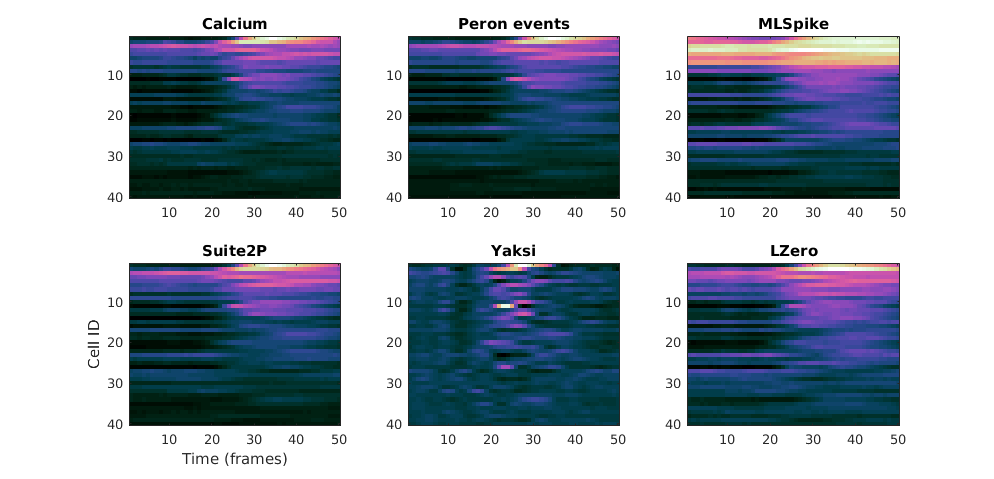
\includegraphics[width=0.9\textwidth]{psth2_40.png}}
%\subfigure[]{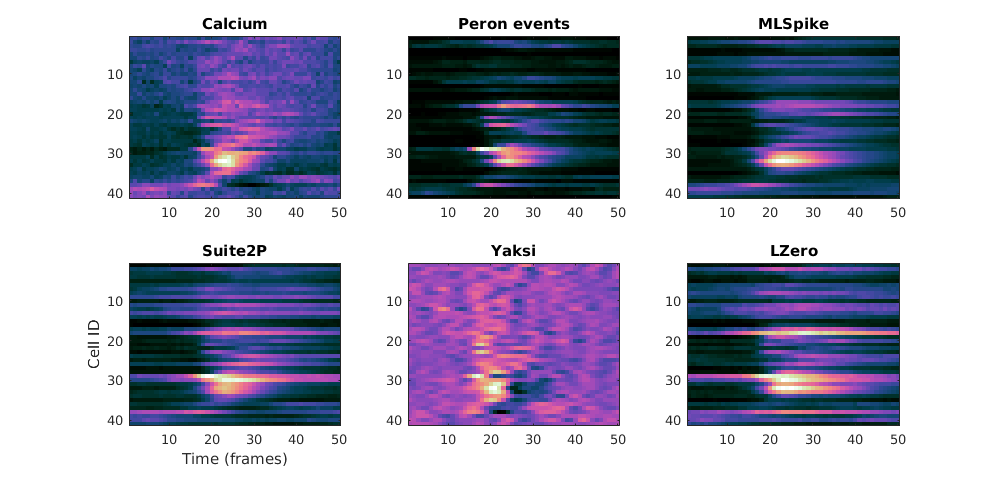
\includegraphics[width=0.9\textwidth]{psth2_720.png}}
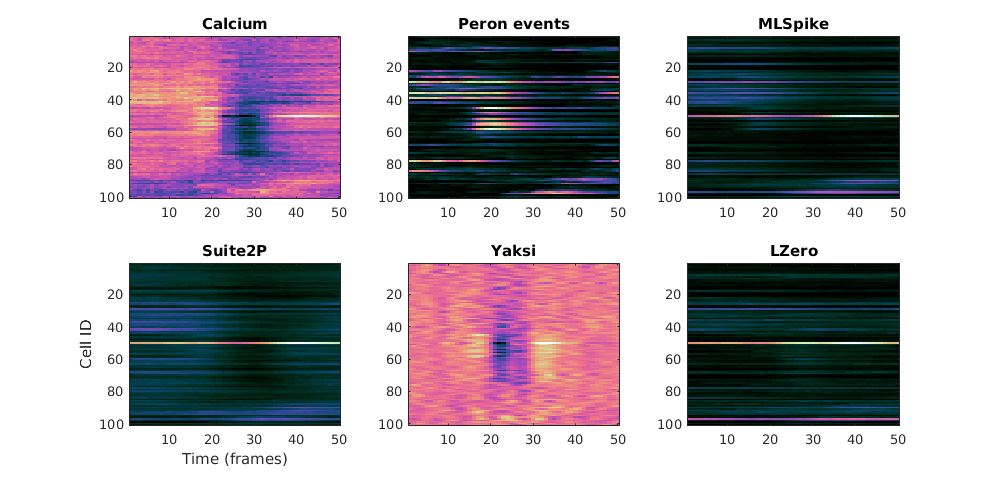
\includegraphics[width=\textwidth]{psth2_1260.png}
\caption{\label{fig:lick_PSTH} PLACEHOLDER FIGURE. Lick induced dip in Ca\textsuperscript{2+} fluorescence seen in the raw Calcium is also seen in deconvolved data.}
\end{figure}

%PSTHs do not show obvious increase in temporal sharpness following deconvolution, but do show signs of missing important features of the data. Each panel shows a different cluster of neurons sorted by t-SNE ordering of PSTHs derived from Calcium data. Pole up is at frame 9, pole down at frame 17, and reward cue is at frame 22. NOTE: Group 3 is aligned to the (likely lick artefact induced) dip in df/f. If this is indeed artifactual, the change in signal still results in a 'rebound' response using Peron (and others, when looking at raw data, figures not shown here)}

%\begin{figure}[h!]
%\centering
%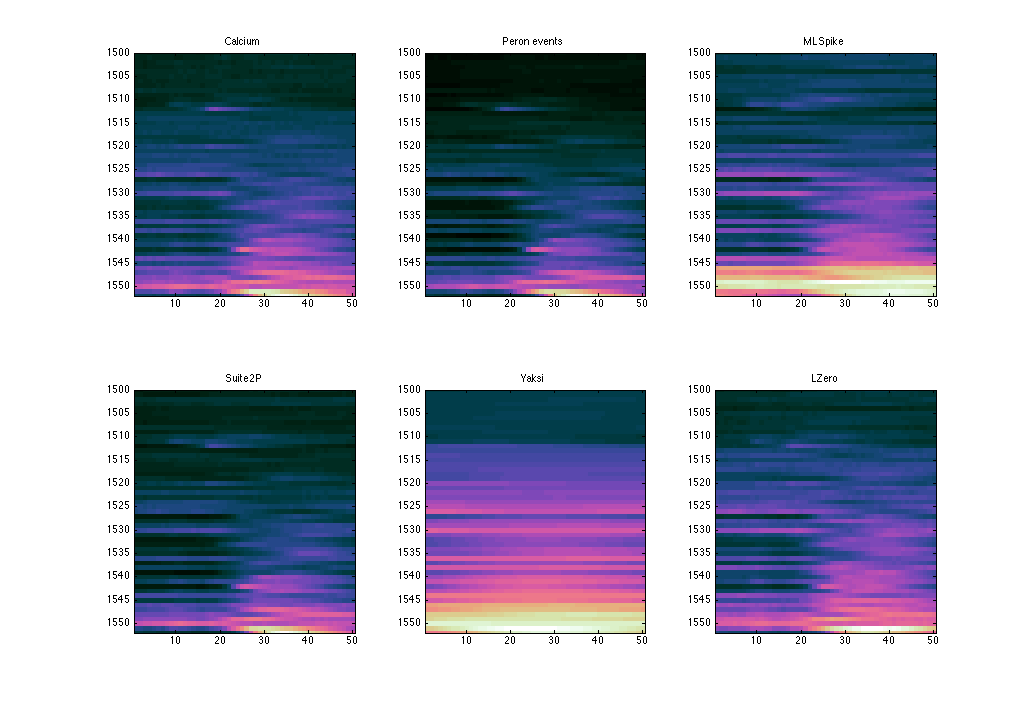
\includegraphics[width=1\textwidth]{psth_all_sorted_zoom2.png}
%\caption{\label{fig:PSTHs}PSTHs do not show increase in temporal sharpness following deconvolution.}
%\end{figure}





%We would expect to do a better job of distinguishing touch vs delay activity or delay vs reward. Is this true?


\section{Discussion}
\emph{MDH NOTES: Add a Discussion to collect notes on what the conclusions and recommendations are e.g.
(1) Don’t use PCC; use ER or something similar (full ROC)}

\emph{(1b) Deconvolution methods trade-off FNs vs FPs (hence need to use metric that captures both)}

PCC is invariant to affine transformations of the data (noted also by \citep{Theis2016-ee}). Specifically, PCC will not change between two cells if the firing rate is doubled or halved. Therefore neither false positives nor false negatives are penalised per se, and spike inference results that maximise PCC between real and inferred spikes cannot be interpreted in terms of spike rate. If the goal of an analysis is to estimate the true firing rate or spike timing of the cell, PCC is not an appropriate metric to use in spike inference optimisation. Instead, a metric such as ER - which explicitly penalises both FPs and FNs, giving better scores to inferred spike trains that are closer to the true spike train in terms of spike count and timing - are a better choice.


\emph{(2) Choice of deconvolution method will change inferences taken from all analyses that follow. So use either (a) raw Ca2+ and deconvolution/spike inference OR (b) two different deconvolution/spike inference methods. [NB this links with ideas of robust inference: that obtaining the same result in the face of wide variation increases its reliability]}

Point to Figure \ref{fig:tuned_cells_psth}

\emph{(3) Message is *not* abandon deconvolution; message is: get it solved. We need these problems solved: when we move to very high frame rate imaging and faster Ca2 sensors, then we will want to look at neural coding at spike resolution. So we will need deconvolution to be properly reliable...}

Many questions do not require spike timing (see short discussion in Harris et al 2016 NN Review `Improving data quality in neuronal population recordings' - \emph{When neurons fire sparsely, for example, neuronal responses can be characterized by how the calcium response itself depends on stimulus or behavioral-related factors. The results of such analyses will not be numerically identical to analyses computed from actual counts (for example when computing correlations among neurons), but if interpreted correctly, this can avoid biases introduced by explicit spike estimation.}). 

(4) Deconvolution and spike inference, and the parameters of the methods used, will affect the signal in predictable ways e.g. more/less FPs/FNs depending on whether you are trying to explain every wrinkle in the Calcium trace vs match empirical firing rate distributions. Correlation distributions will be broader if you've smoothed the signal/ removed noise. So build this understanding into your interpretation.
For example, the dimensionality of the data depends on where you set your spike detection threshold (sparse vs fuller signal), so conclusions about dimensionality need to reflect this.

RE: Pachitariu et al biorxiv 2017 Robustness of spike deconvolution for calcium imaging of neural spiking.
(a) Pachitariu et al 2017 show that PCC between inferred and true spikes can be improved with small modifications to the output of simple non-negative deconvolution algorithms. Shifting spike times by a fixed amount and smoothing the spike count with a gaussian kernel improved PCC - and therefore measured model performance - with no changes to the algorithm. This again suggests PCC is a poor metric for assessing spike inference methods.
(b) Pachitariu et al 2017 suggest a novel metric for assessing spike inference/deconvolution methods in the absence of ground truth. In Pachitariu et al 2017's experiments, an ensemble of stimuli are repeated at least twice, allowing the comparison of deconvolved calcium across stimulus repeats. Algorithms that result in consistent deconvolution traces (similar results on both trials, measured with Spearman's correlation) are rated higher. This approach cannot be applied in many studies. In the Peron dataset described here, and any other studies with unconstrained behaviour of any kind, trial conditions are not precisely repeated. Therefore, consistent deconvolution/ spike inference on different trials are not meaningfully related to better algorithm performance. 

In addition, Pachitariu et al's approach assumes that cells respond consistently on separate trials. This may well be the case in the sensory periphery e.g. Bale et al J.Neuroscience 2015, numerous studies have shown that this is not generally the case e.g. motor studies.


\clearpage
\section{Methods}
\subsection*{Ground truth data}
Ground truth data was accessed from \href{http://crcns.org/data-sets/methods/cai-1}{crcns.org} \citep{Svoboda2015-ym}, and the experiments have been described previously \cite{Chen2013-nv}. Briefly, ...

\subsection*{Spike train metrics}
% NB. script that generates these results is deconv_downsample.m
Pearson correlation coefficient was computed between the ground truth and inferred spike trains following convolution with a gaussian kernel (61 samples wide, 1.02 seconds). \emph{NB this is different to the Spikefinder method of taking the PCC from a downsampled (25Hz) signal, by convolving the spikes with a 40ms square kernel (equivalent to 15 samples here), though the area under both kernels is similar (sum of the gaussian kernel = 18).}\\
Error Rate was computed between the ground truth and inferred spike trains using the \cite{Deneux2016-gu}, implementation of normalised error rate, derived from \cite{Victor1996-cg} Error Rate (code available \href{https://github.com/MLspike}{https://github.com/MLspike}). Briefly, the error rate is 1 - F1-score, where the F1-score is the harmonic mean of sensitivity (number of missed spikes divided by total spikes) and precision (number of falsely detected spikes divided by total detected spikes),
% ($1 - \frac{N missed spikes}{N total spikes}$) and precision ($1 - \frac{N falsely detected spikes}{N detected spikes}$),

\[Error Rate = 1 - 2 \frac{sensitivity \times precision}{sensitivity + precision}.\]

Hits, misses and false detections were counted with a temporal precision of 0.5 seconds.

\subsection*{Parameter fitting}
For each method the best parameters for each cell were determined by brute force search over an appropriate range. The modal best parameters, as determined using Error Rate on downsampled data, were then fixed for the population imaging data analysis. 

In additional tests (TO DO Supplemental figs, subscript 'PCC'), the modal best parameters when assessed using PCC were used, and in the case of MLSpike parameters were additionally hand-tuned using a built-in GUI (TO DO Supplemental figs, subscript 'hand'). 

%the only hand tuned method was MLSpike, and for that there’s a GUI where you fiddle with the parameters until you get a result that ‘looks right’. For the first two figures I did a parameter sweep for all three methods. Then in the later figures I either did the ‘eyeball’ fiddling on a few neurons to get an idea of the best params (MLSpike) or I took the parameters that produced the best performance when optimizing ER or PCC. This is stated in the subscript of each method in figure 4. By ‘best’ I took the modal best params across the 21 cells in the ground truth case I.e. the consensus best params

\subsection*{Downsampling}
Ground truth calcium data was downsampled from 60Hz to 7Hz in Matlab by up-sampling by 7 - {\tt{interp(ca,7)}} and downsampling the resultant signal by 60, as Matlab's downsampling must be done in integer steps.

\subsection*{Peron data description}
Experiment overview. 

Data prep.

\subsection{Event rate estimation}
Spike inference methods (Suite2P$_{events}$,MLSpike$_{events}$, LZero$_{events}$) return estimated spikes which were converted into mean event rates (Hz) per cell. Event rate for continuous methods (Calcium, Peron, Yaksi, Suite2P$_{kernel}$,MLSpike$_{kernel}$, LZero$_{kernel}$) for each cell was determined by counting activity/fluorescence events greater than three standard deviations of the background noise. Background noise was calculated by taking a four-point moving average and subtracting this from the activity/fluorescence trace. Event rate was then computed in Hz.

Silent cells were defined as cells with event rates below 0.0083Hz (or fewer than one spike per two minutes of recording) as in \citep{OConnor2010-hd}.

\subsection{Tuned cells}
Following Peron

Tuned cell agreement.

\subsection{Touch-related responses}
Touch-tuned cells were determined by computing touch-triggered average activity for each cell, before calculating whether the data distribution of peak touch-induced activity exceeds the expected activity of shuffled data. In more detail, the time of first touch - between the mouse's whisker and the metal pole - on each trial was recorded. For each touch time one second (seven data samples) was extracted before and after the frame closest to touch (15 samples total), and the mean activity was calculated. The time of peak touch-triggered average activity was calculated, and a ranksum test (bonferroni corrected) between the true data distribution at peak time and a matched random sample of data from the same cell. This test determined whether peak touch-triggered activity was significantly different from chance. 


\subsection{Pairwise correlations}
Pairwise correlations were calculated for all pairs of neurons in Matlab (corrcoef) at the data sampling rate (7Hz). Correlations between correlation matrices (Fig. \ref{fig:cxy_comparison}) were computed between the unique pairwise correlations from each method (i.e. {\tt CXY(find(triu(CXY)))}).

Random data surrogates: \\ 
\indent - Shifted: the fluorescence time series for each cell was randomly shifted in time (using Matlab's circshift function) by up to 10000 frames. LOGIC: to preserve each cell's autocorrelation\\
\indent - Scrambled - elements of the original N x T data matrix were sampled randomly (without replacement) to generate a new data matrix. LOGIC: keep true data distribution but randomize everything else\\
\indent - Randn - pseudorandom values drawn from a normal distribution. LOGIC: Totally random. N.B. Key here is the scrambled data is identical, as PCC doesn't care about the data distribution per se, only the covariability in the data i.e. they both go up, regardless of whether it's a twofold or a tenfold increase\\
\indent - Conv (kernel) - original data convolved with an exponentially decaying kernel as is used in the MLSpike and Suite2P deconvolution methods. LOGIC: to show the effect that smoothing has on the correlation distribution \\
\indent - Shuffled rows - like the 'scrambled' data, but shuffling was done separately for each cell (rows of the data matrix). LOGIC: to preserve differences in event rate across neurons. Again, this shouldn't be any different to the scrambled data as PCC is invariant to affine transformations i.e. same tuning but larger changes in firing rate.\\


\subsection{Dimensionality}
To determine the dimensionality of each dataset we performed eigendecomposition of the covariance matrix of each dataset. The resultant eigenvalues were sorted into descending order, and the variance explained ({\tt cumsum(egs)/sum(egs)}) plotted.


\subsection*{List of deconvolution methods}
\subsubsection*{Suite2P}
\texttt{Suite2P} (\href{https://github.com/cortex-lab/Suite2P}{https://github.com/cortex-lab/Suite2P}) is actively developed by  Marius Pachitariu and members of the cortexlab (Kenneth Harris and Matteo Carandini) at UCL. Suite2P's USP is it's application to large scale 2-photon imaging analysis, with an emphasis on end-to-end processing (images to neural event time series) and speed. A preprint describing the toolbox is available here:\\

\noindent \href{http://biorxiv.org/content/early/2016/06/30/061507}{http://biorxiv.org/content/early/2016/06/30/061507}, \\

\noindent and our own notes on the spike detection algorithm are here:\\

\noindent \href{https://drive.google.com/open?id=1NeQhmoRpS-x8R0e84w3TqkUR1PNMXiem6ZIjJta-U7A}{https://drive.google.com/open?id=1NeQhmoRpS-x8R0e84w3TqkUR1PNMXiem6ZIjJta-U7A}.

\subsubsection*{MLSpike}
\texttt{MLSpike} (\href{https://github.com/mlspike}{https://github.com/mlspike}) was developed by Thomas Deneux at INT, CRNS Marseille, France. A model-based probabilistic approach, \texttt{MLSpike} was developed to recover spike trains in calcium imaging data by taking baseline fluctuations and cellular properties into account. A comprehensive explanation of the algorithm and its benefits can be found in the paper:\\

\noindent Deneux, Thomas, Attila Kaszas, Gergely Szalay, Gergely Katona, Tamás Lakner, Amiram Grinvald, Balázs Rózsa, and Ivo Vanzetta. "Accurate spike estimation from noisy calcium signals for ultrafast three-dimensional imaging of large neuronal populations in vivo." Nature Communications 7 (2016).\\

\noindent Link: \href{https://www.nature.com/articles/ncomms12190}{https://www.nature.com/articles/ncomms12190}

MLSpike can return a maximum a posteriori spike train, or a spike probability per time step. We show results for both denoted MLSpike$_{events}$ and MLSpike$_{pspike}$

\subsubsection*{LZero}
The method we refer to as \texttt{LZero} was developed by Sean Jewell and Daniela Witten from U.Washington, Seattle, USA. The goal for this implementation was to cast spike detection as a change-point detection problem, which could be solved with an existing $l_{0}$ optimization algorithm. In their paper Jewell and Witten show that the $l_{0}$ solution is better than previously implemented $l_{2}$ solutions, with results much closer to the real spike train ($l_{2}$ solutions tend to overestimate the true firing rate). Details can be found in the paper:\\

\noindent Jewell, Sean, and Daniela Witten. "Exact Spike Train Inference Via $l_{0}$ Optimization." arXiv preprint arXiv:1703.08644 (2017).\\

\noindent Link: \href{https://arxiv.org/abs/1703.08644}{https://arxiv.org/abs/1703.08644}

\subsubsection*{Yaksi}
\texttt{Yaksi} refers to the `vanilla' deconvolution of Yaksi and Friedrich (2006). This is to be used as a baseline for comparison with more sophisticated methods. \st{\textbf{\emph{NOTE 8.6.17}} my implementation results in signals that are more temporally smooth (as opposed to more temporally sharp) than the calcium signal, indicating the filtering has not been performed properly.} \\

\noindent The method is detailed in the paper: \\
\noindent Yaksi, Emre, and Rainer W. Friedrich. "Reconstruction of firing rate changes across neuronal populations by temporally deconvolved Ca2+ imaging." Nature Methods 3, no. 5 (2006): 377-383.


\subsubsection*{Peron events}
\texttt{Peron events} refer to the extracted events detailed in the original \emph{Peron et al. 2015} paper. It is a version of the 'peeling' algorithm tuned to generate a low number of false positive detections (a rate of 0.01Hz) on ground truth data, leading to a hit rate of 54$\%$

\noindent Peron, Simon P., Jeremy Freeman, Vijay Iyer, Caiying Guo, and Karel Svoboda. "A cellular resolution map of barrel cortex activity during tactile behavior." Neuron 86, no. 3 (2015): 783-799.

\subsubsection*{Events + kernel versions}
Where a spike inference method returns spike rates per time point, these are plotted as Method$_{events}$. To compare to other methods that return a de-noised df/f or firing rate estimate, these events are convolved with a calcium kernel and plotted as Method$_{kernel}$.

\clearpage
\beginsupplement
\section{Supplemental}

\begin{figure}[h!]
%\floatbox[{\capbeside\thisfloatsetup{capbesideposition={right,top},capbesidewidth=0.4\textwidth}}]{figure}[\FBwidth]
{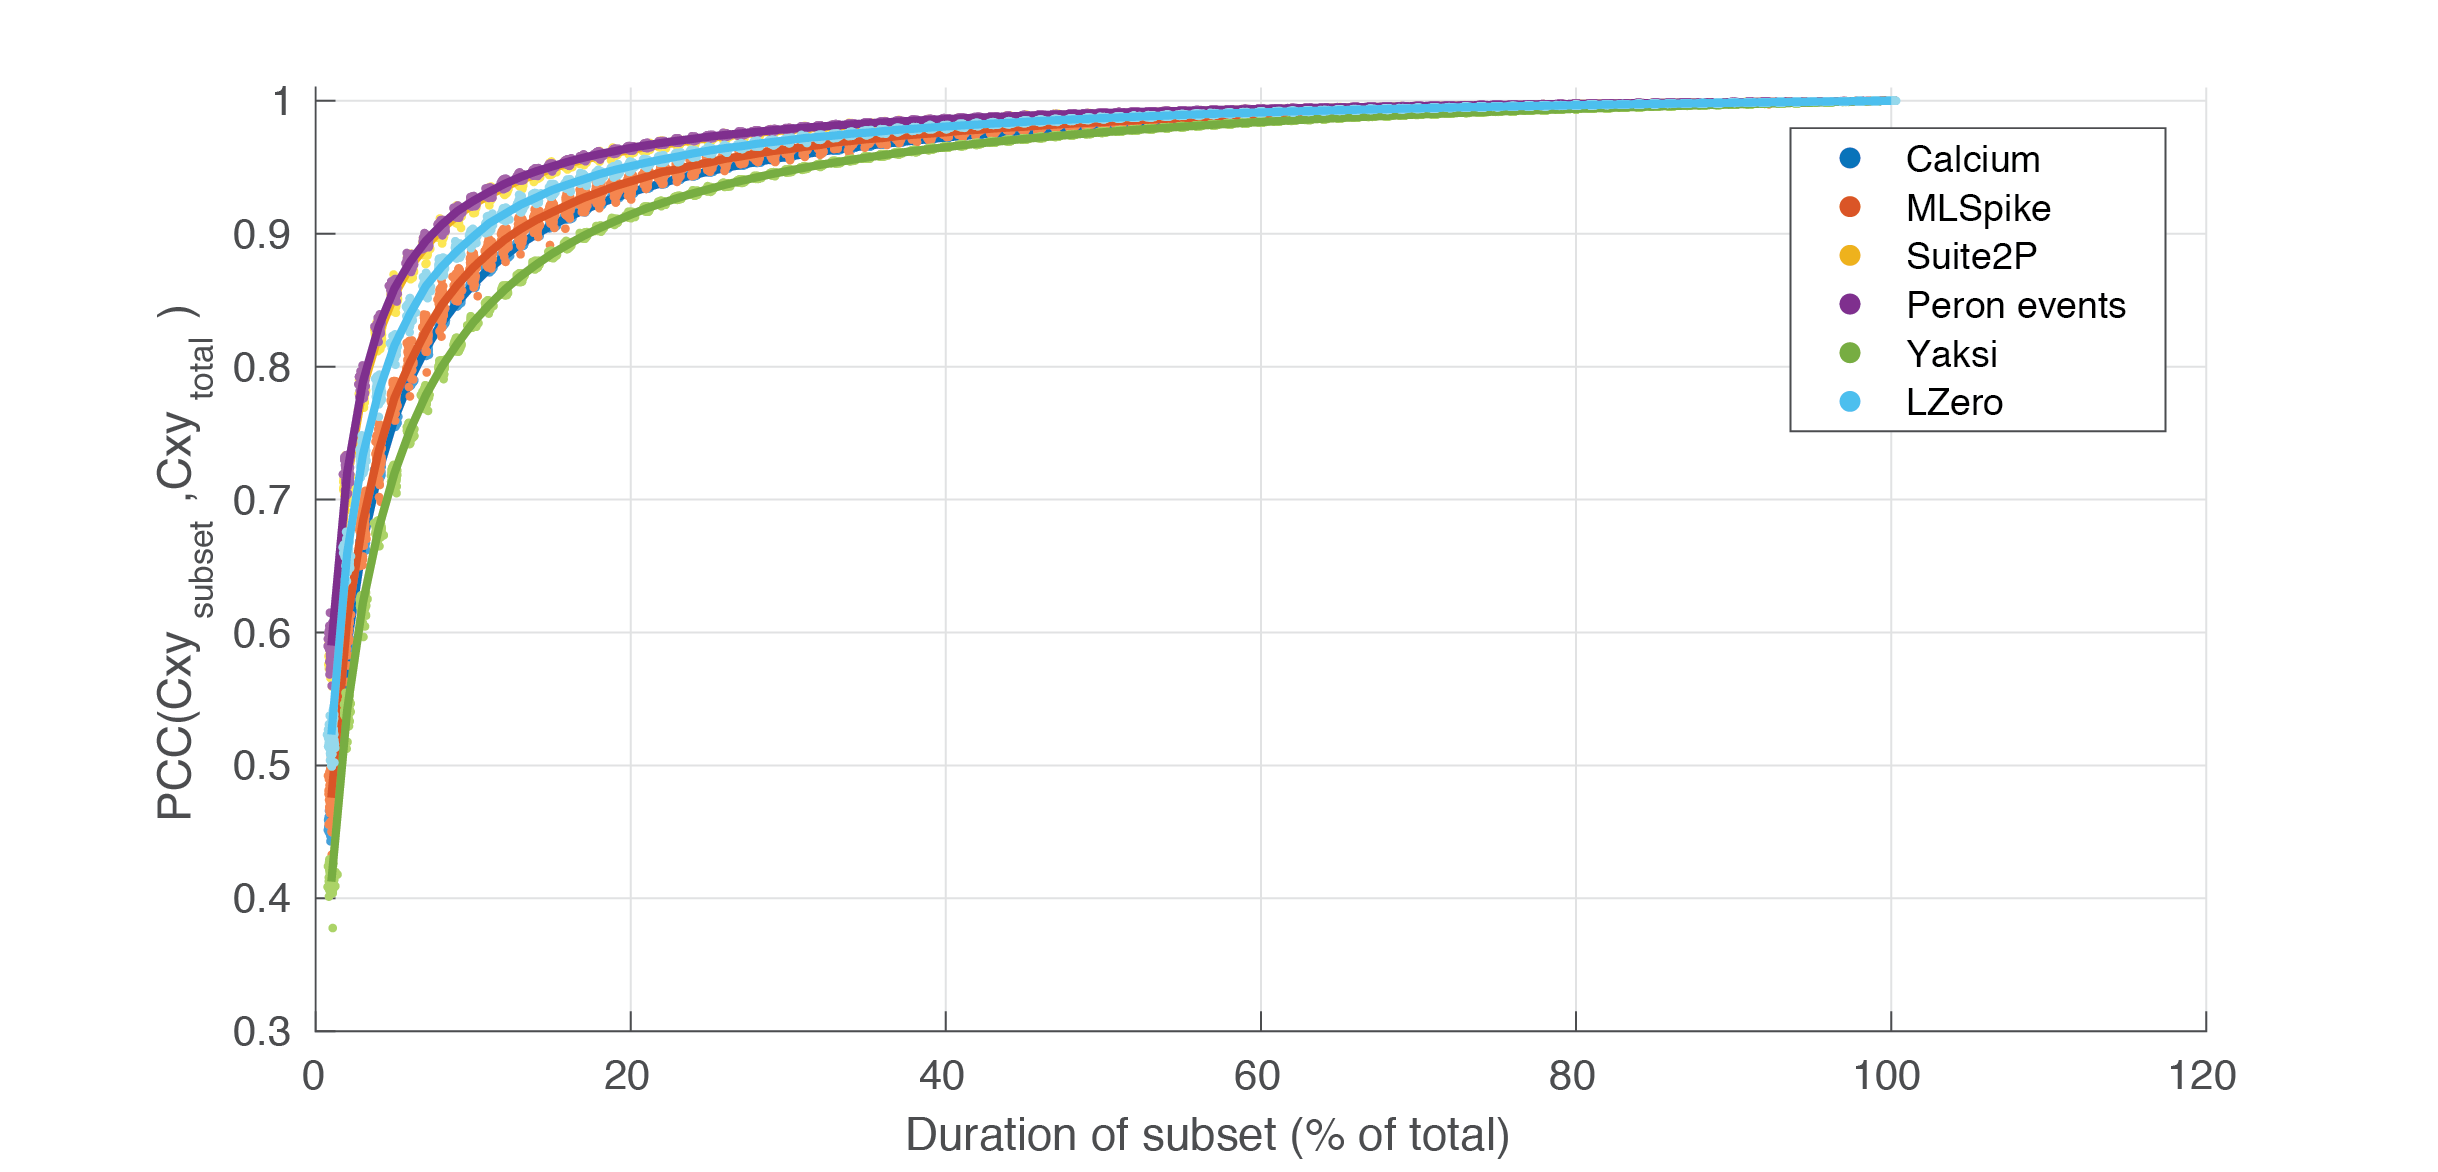
\includegraphics[trim={30 20 60 20},clip,width=\textwidth]{figs/cxy_subset_comparison3.png}}
{\caption{\label{fig:supp_cxy_stability}Example datasets are long enough to generate stable correlation estimates. Correlation between the pairwise correlation matrix for a given method, and an equivalent correlation matrix for subsets of the data. For each datapoint in the figure a subset (1\%-100\%) of the full dataset is extracted at random without replacement and a matrix of pairwise correlations is generated. These correlations are then compared to the matching pairwise correlations in the full dataset. In all instances 20\% of the data is sufficient to recover correlations of 0.9, though there is substantial variation between methods.}}%(b) Pairwise correlation matrix between correlation matrices for each method.}
\end{figure} % Code for this plot is in compare_peron.m


%\begin{figure}[h!]
%\centering
%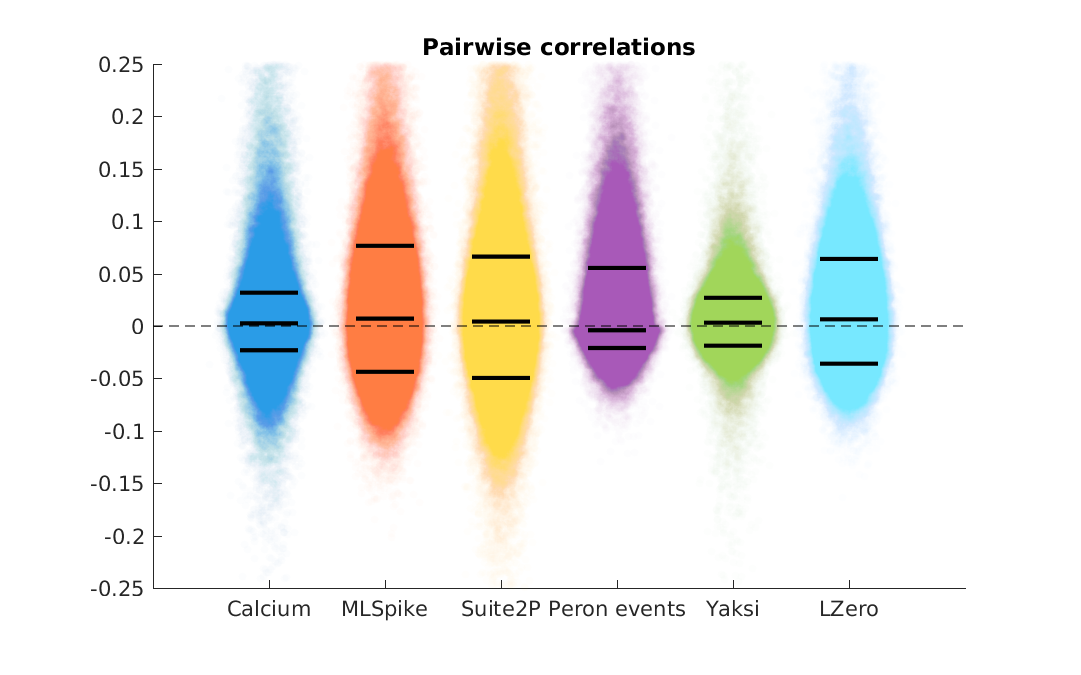
\includegraphics[width=0.9\textwidth]{pairwise_scatter3_alph_pt01_zoom.eps}
%\caption{\label{fig:PCCs_zoom}Zoomed in version of \ref{fig:PCCs} }
%\end{figure}

%\begin{figure}[h!]
%\centering
%\subfigure{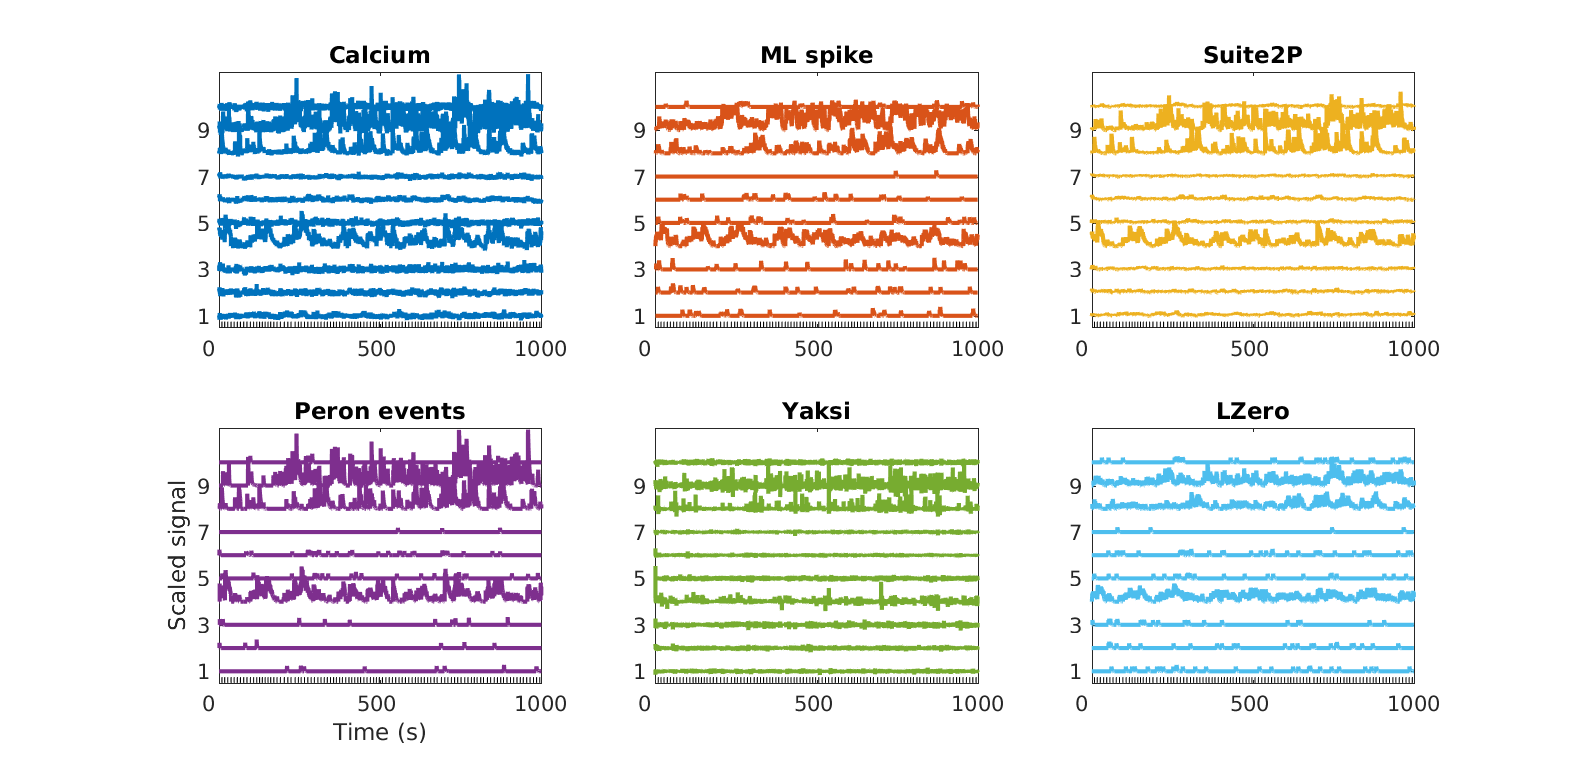
\includegraphics[width=0.9\textwidth]{10cells_compare2.eps}}
%\subfigure{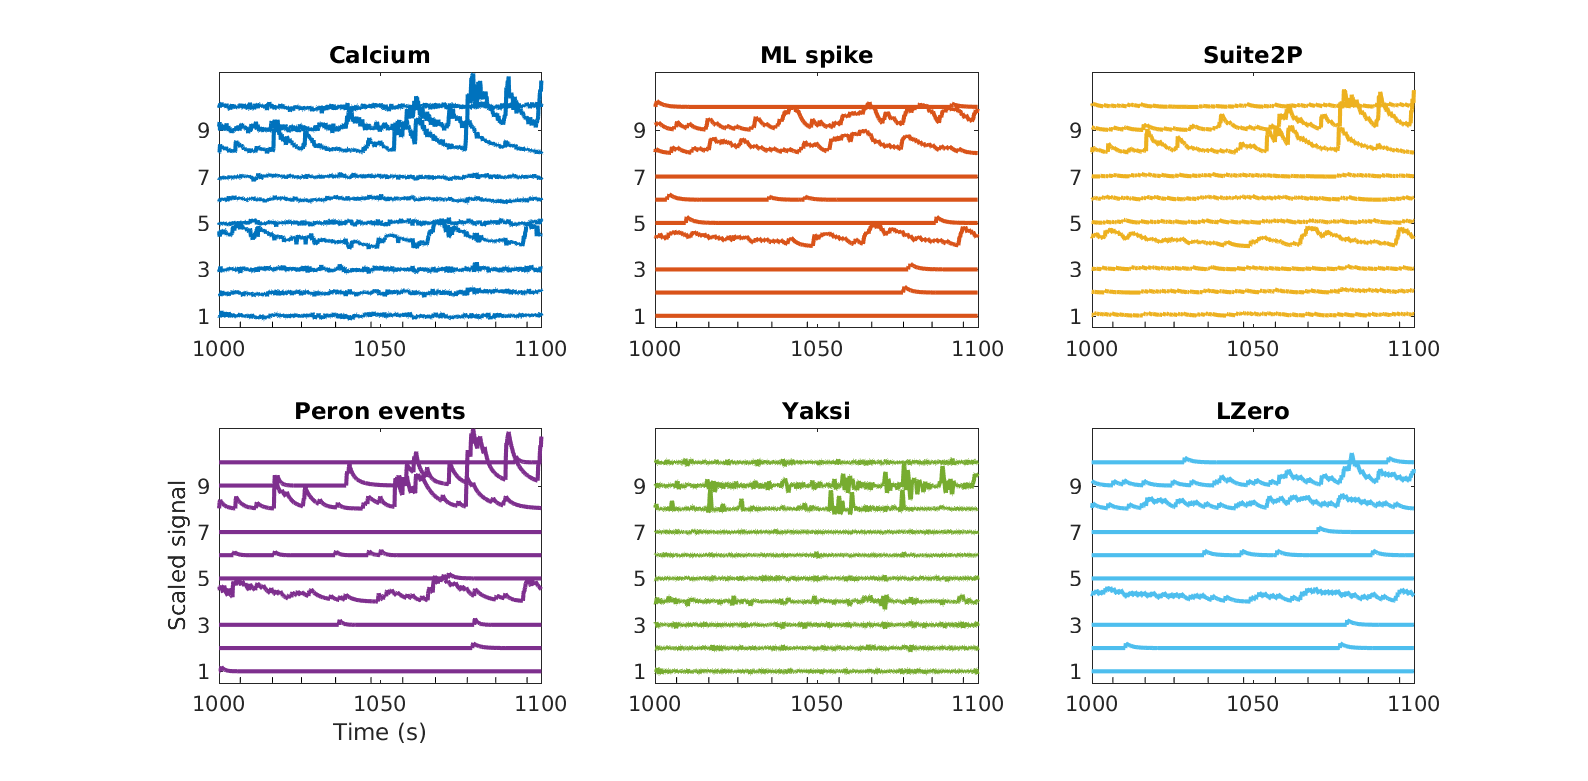
\includegraphics[width=0.9\textwidth]{10cells_compare2_zoom.eps}}
%\subfigure{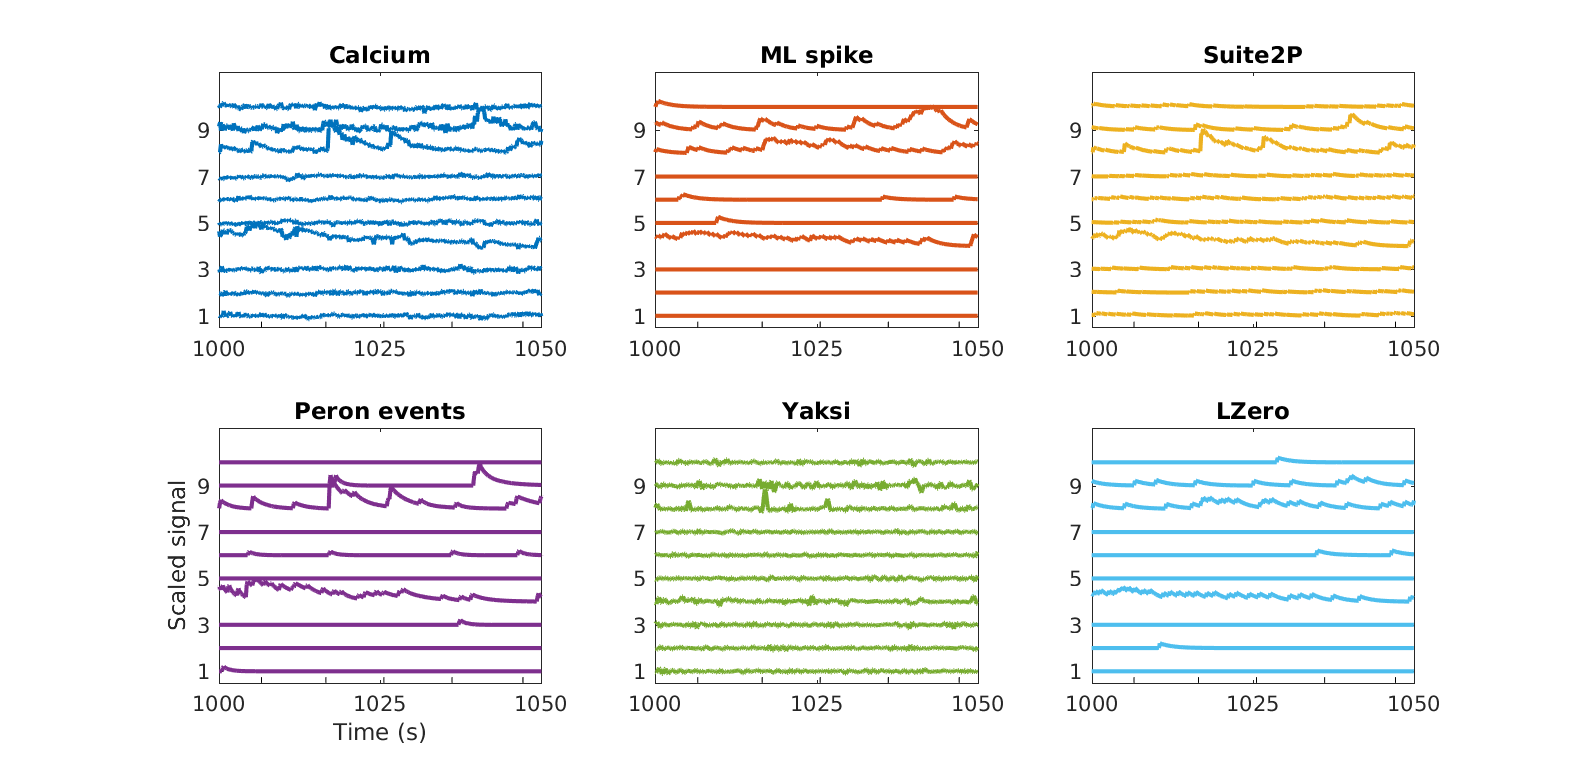
\includegraphics[width=0.9\textwidth]{10cells_compare2_zoom2.eps}}
%\caption{\label{fig:raw1}Example deconvolution for 10 cells using each method. Different figures are the same data at increasing levels of zoom.}
%\end{figure}

%\begin{figure}[h!]
%\centering
%\subfigure{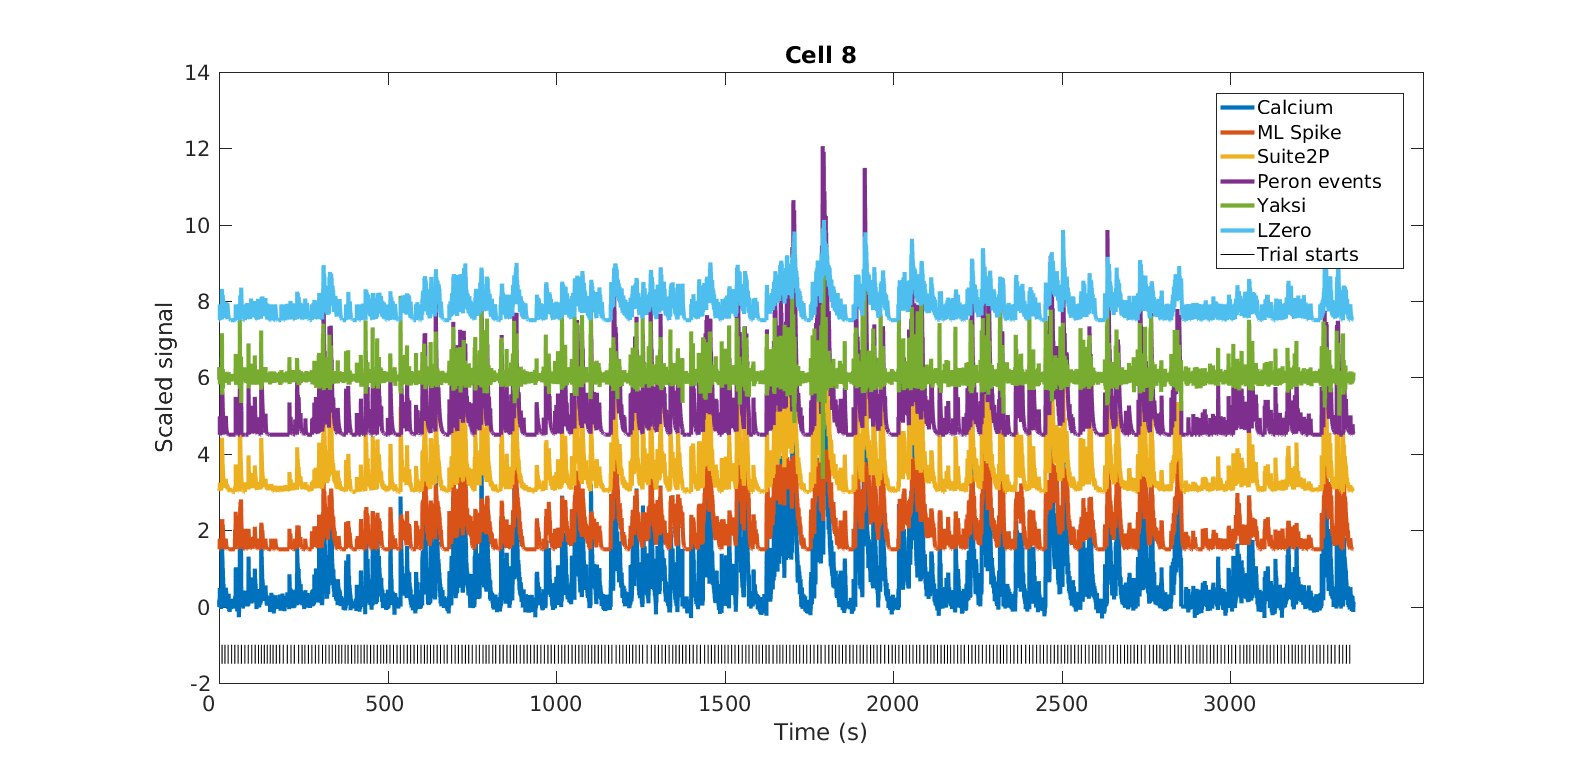
\includegraphics[width=0.75\textwidth]{cell8_deconv_compare2.eps}}
%\subfigure{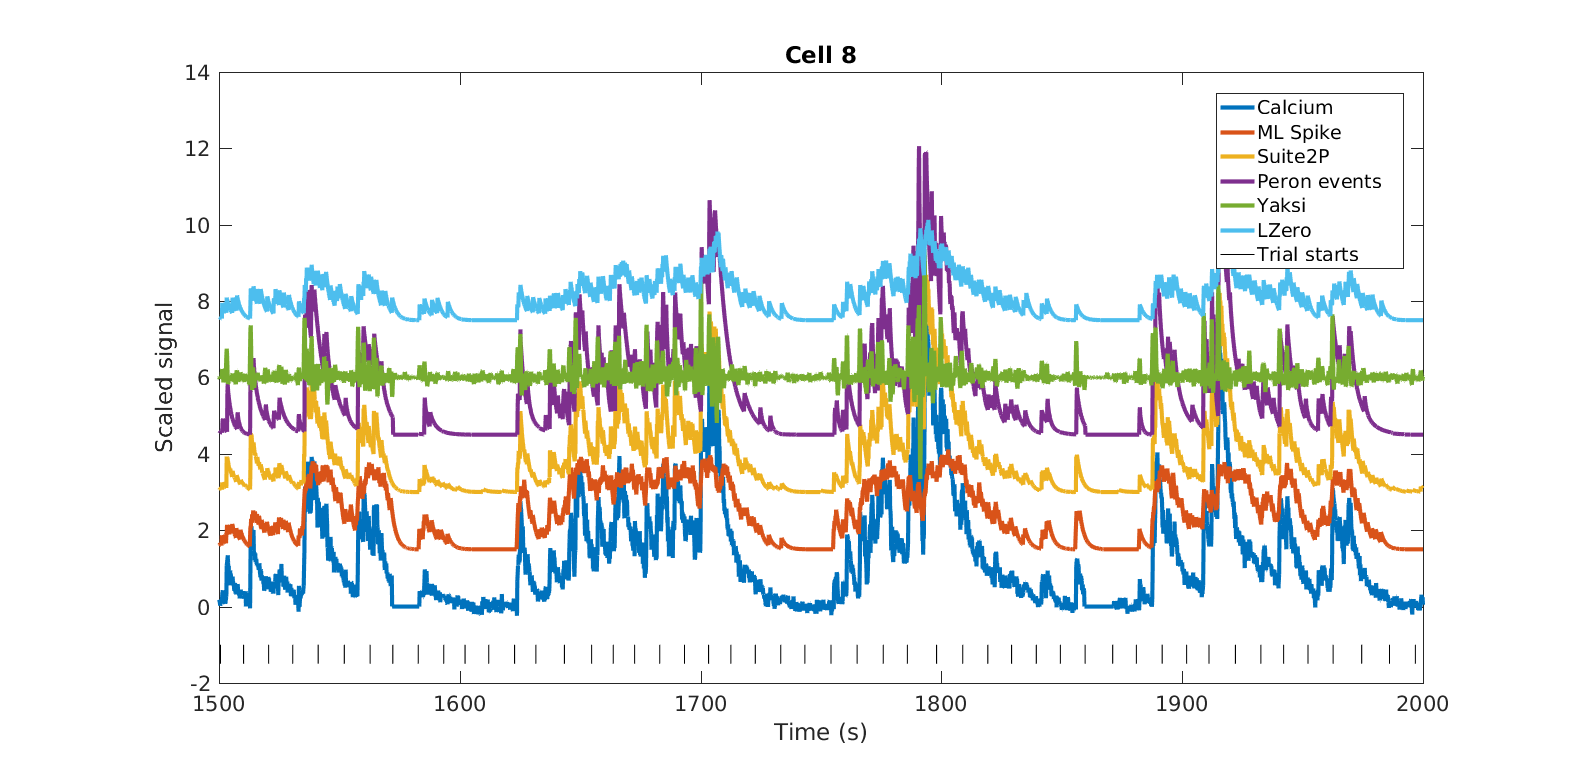
\includegraphics[width=0.75\textwidth]{cell8_deconv_compare2_zoom1.eps}}
%\subfigure{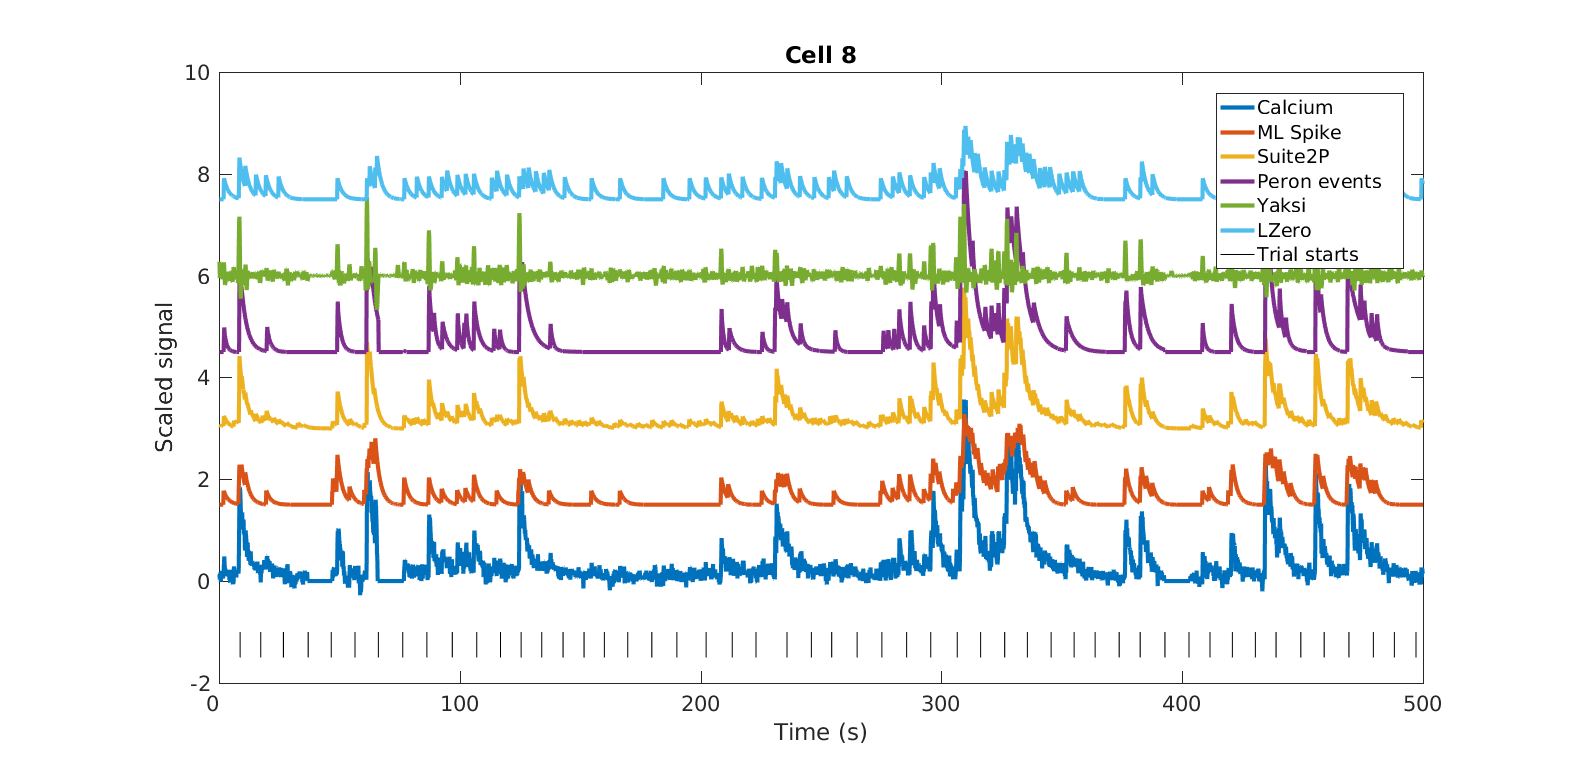
\includegraphics[width=0.75\textwidth]{cell8_deconv_compare2_zoom2.eps}}
%\subfigure{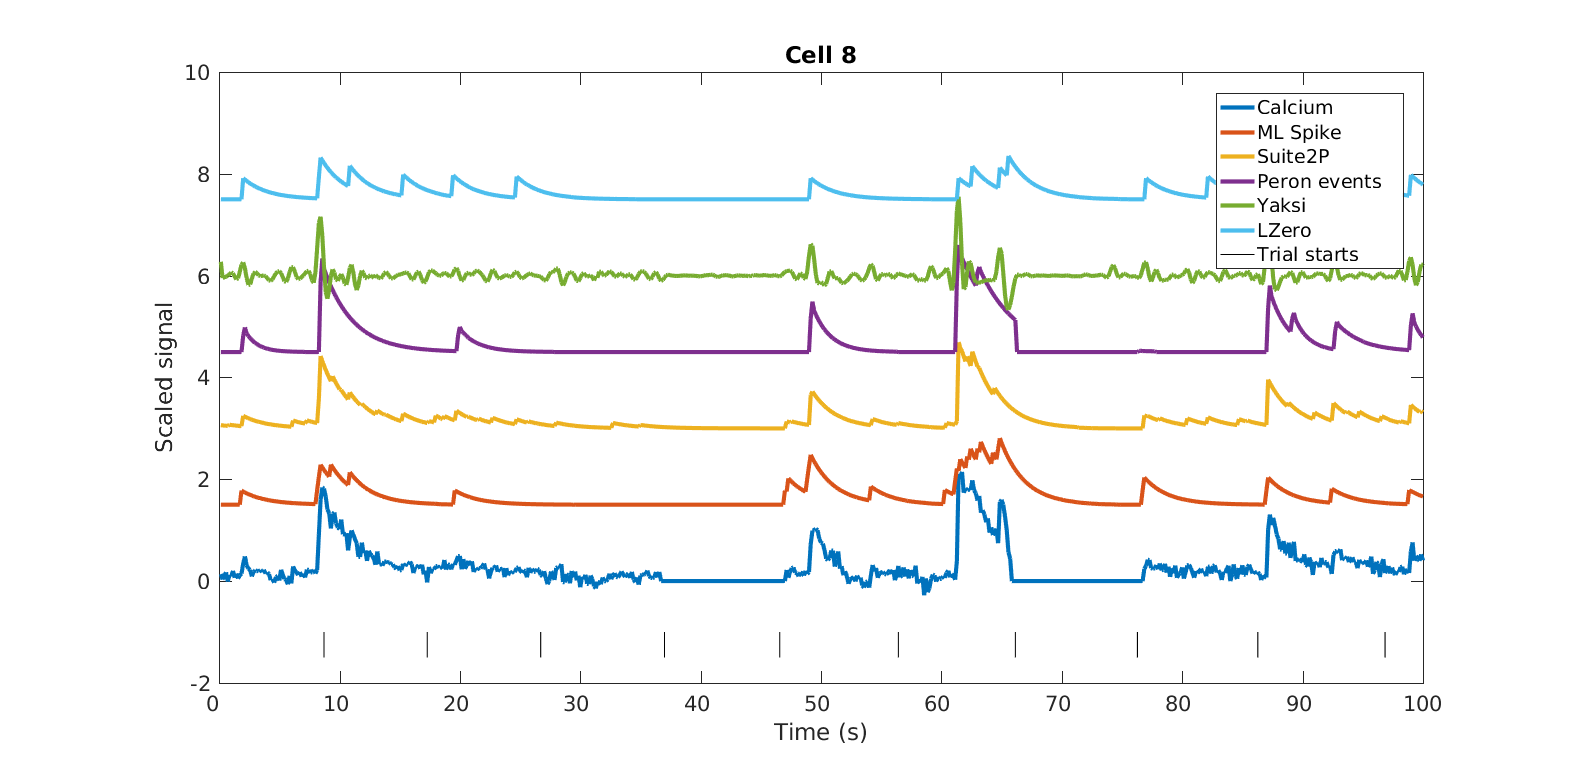
\includegraphics[width=0.75\textwidth]{cell8_deconv_compare2_zoom3.eps}}
%\caption{\label{fig:raw1}Example deconvolution for one cell using each method. Different figures are the same data at increasing levels of zoom.}
%\end{figure}



% \subsection{How to add Citations and a References List}

% You can upload a \verb|.bib| file containing your BibTeX entries, created with JabRef; or import your \href{https://www.overleaf.com/blog/184}{Mendeley}, CiteULike or Zotero library as a \verb|.bib| file. You can then cite entries from it, like this: \cite{greenwade93}. Just remember to specify a bibliography style, as well as the filename of the \verb|.bib|.

% You can find a \href{https://www.overleaf.com/help/97-how-to-include-a-bibliography-using-bibtex}{video tutorial here} to learn more about BibTeX.

% We hope you find Overleaf useful, and please let us know if you have any feedback using the help menu above --- or use the contact form at \url{https://www.overleaf.com/contact}!

 \bibliographystyle{plainnat}
 \bibliography{references.bib}

\end{document}